% Document Class and Basic Packages
%-------------------------------------------------------------------------------
\documentclass[letterpaper,11pt]{article} % Define the document class and options
\usepackage{graphicx} % For including graphics
\usepackage[margin=1in]{geometry}
\usepackage{cite} % Handle citations
\usepackage[final]{hyperref} % Add hyperlinks
\usepackage{pgfplotstable, booktabs} % Enhance table handling
\usepackage{multirow}
\usepackage{placeins} % Control float placement
\usepackage{tabularray} % Advanced tables
\usepackage{titlesec} % Customize section titles
\usepackage{fancyhdr} % Create custom page headers and footers
\usepackage{empheq} % Highlight equations
\usepackage{amssymb} % Extended math symbols
\usepackage{tcolorbox} % Colored boxes
\usepackage{enumitem} % Enhanced list environments
\usepackage{xcolor} % Define custom colors
%\usepackage{parskip} % Adjust paragraph spacing
\usepackage{siunitx} % Handling SI units
\usepackage{cancel} % Strikethrough text
\usepackage{listings} % Include code listings
\usepackage{tocloft}  % Table of contents formatting
\usepackage{mathtools}
\usepackage{pdfpages}
\usepackage{times}
%\usepackage{mathastext}
\usepackage{color}
\usepackage{amsmath}
\usepackage{longtable} % Multipage tables

% Long table caption settings
\setlength{\LTcapwidth}{\textwidth} % Width of long table caption


% 1.5 spacing equivalent to word
\usepackage{setspace}
\linespread{1.25}

%\graphicspath{{Sections/Figures/}}

% Better texttt
\newcommand{\opus}[1]{%
  \begingroup
    \spaceskip=\fontdimen2\font plus \fontdimen3\font minus \fontdimen4\font
    \xspaceskip=\fontdimen7\font\relax
    \ttfamily
    %\hyphenchar\font=`\-
    #1%
  \endgroup
}

% Define Custom Colors
%-------------------------------------------------------------------------------
\definecolor{codegreen}{rgb}{0,0.6,0}
\definecolor{codegray}{rgb}{0.5,0.5,0.5}
\definecolor{codepurple}{rgb}{0.58,0,0.82}

% Define Code Listing Style
%-------------------------------------------------------------------------------
\lstdefinestyle{mystyle}{
    commentstyle=\color{codegreen},
    keywordstyle=\color{codepurple},
    numberstyle=\tiny\color{codegray},
    stringstyle=\color{codegreen},
    basicstyle=\ttfamily\small,
    breakatwhitespace=false,         
    breaklines=true,                 
    captionpos=b,                    
    keepspaces=true,                                                     
    showspaces=false,                
    showstringspaces=false,
    showtabs=false,                  
    tabsize=4
}

\DeclarePairedDelimiter\abs{\lvert}{\rvert}%
\DeclarePairedDelimiter\norm{\lVert}{\rVert}%

% Swap the definition of \abs* and \norm*, so that \abs
% and \norm resizes the size of the brackets, and the 
% starred version does not.
\makeatletter
\let\oldabs\abs
\def\abs{\@ifstar{\oldabs}{\oldabs*}}
%
\let\oldnorm\norm
\def\norm{\@ifstar{\oldnorm}{\oldnorm*}}
\makeatother

% Set Code Listing Style
\lstset{style=mystyle}

% Define Custom Commands and Settings
%-------------------------------------------------------------------------------
\newcommand*\widefbox[1]{\fbox{\hspace{0em}#1\hspace{0em}}} % Create a wide box
\newcommand{\tr}{\text{tr}} % Define a trace command for math mode

% Page Header and Footer Setup
%-------------------------------------------------------------------------------
\pagestyle{fancy} % Use the fancy page style
\fancyhf{} % Clear all header and footer fields
\fancyhead[L]{MEC E 403} % Left-aligned header
\fancyhead[C]{Lab 1: Centrifugal Pumps} % Center header
\fancyhead[R]{Alex Diep} % Right-aligned header
\fancyfoot[C]{\thepage} % Centered page number in the footer

% Section and Subsection Formatting
%-------------------------------------------------------------------------------
\titleformat*{\section}{\Large\bfseries} % Customize section titles
\titleformat*{\subsection}{\large\bfseries} % Customize subsection titles
%\renewcommand{\thesection}{Question \arabic{section}} % Modify section numbering
%\renewcommand{\thesubsection}{(\alph{subsection})} % Modify subsection numbering

% Hyperlink Setup
%-------------------------------------------------------------------------------
\hypersetup{
	colorlinks=true, % Enable colored links
	linkcolor=blue, % Set link color
	citecolor=blue, % Set citation color
	filecolor=magenta, % Set file link color
	urlcolor=blue % Set URL link color
}

% Indentation Setup
%-------------------------------------------------------------------------------
%\newcommand{\forceindent}{{\setlength{\parindent}{2em}\indent}}

% Custom SI Unit Definitions
\DeclareSIUnit\LSB{LSB} % Least significant bit
\DeclareSIUnit{\lb}{lb} % Pound
\DeclareSIUnit{\psi}{psi} % Psi
\DeclareSIUnit{\rpm}{RPM} % Revolutions per minute

% Custom Table of Contents Formatting
\renewcommand\cftsecdotsep{\cftdot} % Use dots for section 
\renewcommand{\cftsecleader}{\cftdotfill{\cftsubsecdotsep}} % Use subsection dots for section

% Siunitx Setup
\sisetup{group-digits=false} % 666.666 -> 666666 for \qty
\sisetup{detect-all} % Something to do about unit font and document font
%\sisetup{per-mode=fraction} % Fractions for per unit typesetting

% \titlespacing\section{0pt}{12pt plus 4pt minus 2pt}{0pt plus 2pt minus 2pt}
% \titlespacing\subsection{0pt}{12pt plus 4pt minus 2pt}{0pt plus 2pt minus 2pt}
% \titlespacing\subsubsection{0pt}{12pt plus 4pt minus 2pt}{0pt plus 2pt minus 2pt}
\titlespacing*{\section}{0pt}{0.1\baselineskip}{0.2\baselineskip}
\titlespacing*{\subsection}{0pt}{0.1\baselineskip}{0.2\baselineskip}
\titlespacing*{\subsubsection}{0pt}{0.1\baselineskip}{0.2\baselineskip}

% Define Custom Table Column Types
\newcolumntype{C}[1]{>{\centering\arraybackslash}p{#1}}

% End of Preamble
%-------------------------------------------------------------------------------

%++++++++++++++++++++++++++++++++++++++++
\begin{document}

\begin{titlepage}
    \centering
    \vspace*{2cm} % Adjust vertical spacing
    
    % Title
    \Huge {MEC E 403 \\Lab 1: Centrifugal Pumps} \\
    \vspace{1cm} % Adjust vertical spacing
    
    % Author
    \Large by: Alex Diep \\
    \vspace{1cm} % Adjust vertical spacing

    % Date
    \Large Date: March 1, 2023 \\ % or manually specify a date
    \vspace{2cm} % Adjust vertical spacing

    \begin{table}[h]
        \centering
        \begin{tabular}{ll}
            Instructor & Lisa Kinsale \\
            TAs & Enrique Millones \\
            & Simin Shabani \vspace{0.5cm} \\
            Group Members & Ahmad, Safiya \\
            & Allegretto, Luca \\
            & Colabella, James \\
            & Dadhania, Karan \\
            & Sammam, S M Faiaz \vspace{0.5cm} \\
            CCID & abdiep \\
            Student ID & 1664334 \\
            Section & H41 \\
            Group & 13 \\
        \end{tabular}
    \end{table}
    \begin{figure}[h]
        \centering
        
\includegraphics[width=0.2\textwidth]{uofa_engineering_logo.png}
    \end{figure}
    \vfill % Fill vertical space

    
\end{titlepage}
\renewcommand\arraystretch{1.5}

% no page number or abstract
\pagenumbering{gobble}

%\begin{abstract}
\section*{Abstract}
    Bolted connections are integral components in various engineering structures, facilitating disassembly without damage and offering versatility in construction. Understanding their mechanics is paramount for ensuring structural integrity and reliability in engineering applications. This study investigates bolted connections, examining key parameters such as modulus of elasticity, preload, stress and strain, washer calibration, torque coefficient, bolt stiffness, and member stiffness. Through experimentation and analysis, this research seeks to understand the mechanics of bolted connections, providing groundwork for future reliable engineering practices.

    The experimental investigation involved utilizing an MTS testing machine and instrumented bolted joints, including strain conditioner and gauges, and a torque wrench. Six tests were conducted: zero preload, torque test (zero external load), repeated loading, static loading, shake down, and dynamic loading. 

    Results from the zero preload trial indicate a modulus of elasticity of $205 \pm 4.70$ GPa, a bolt calibration of $\varepsilon_{b} = 8.47E-05 P$, preload uncertainty of $\pm 5\%$ kN, and washer calibration of $-2.11 \times 10^{-1}P$. From the geometry of the bolt and $E_b$, the stiffness was determined to be $k_b = 209$ MN/m.
    
    Results from the zero load trial found torque coefficient, $K = 0.167$, which falls within the expected range of $0.1 - 0.2$. 
    
    The uncertainty for the bolt transducer reading was determined from a repeatability test to be $\delta V_{o, b} =\pm 0.03$
    
    Next, assuming the stress distribution was $45^{\circ}$, the theoretical stiffness of the joined members was determined to be $k_{m, \text{th}} = 2222$ MN/m. The static loading trials found the experimental stiffness of the joined members to be $k_{m, \text{exp}} = 1600$ MN/m. The relative error between the theoretical and experimental  stiffness of the member was $28.0\%$. 

    From the static loading trials, the separation point for the bolt without a gasket was found to be $P = 4.98$ kN experimentally and $P = 4.67$ kN theoretically, with a $6.78\%$ relative error. It was observed that the gasket decreased the bolt force for a given external load, and the gasket helped prevent the members from separating.

    The study also found that both the mean and alternating stresses increased as torque increased. The gasket generally increased the mean stress and alternating stress. The alternating stress decreased as torque increased, and the mean stress increased as torque increased.

    This report gave insight to the loading patterns experienced by bolts and the resulting changes induced by varying parameters on connection stress. This may serve as a reference of understanding to compliment the theory behind bolted connections, the fundamentals of strength testing, diverse loading methodologies, the significance of preload, disparities between members with and without a gasket, and the interrelationships among pertinent parameters.
%\end{abstract}
\newpage
% use roman numerals for page numbers in table of contents
\pagenumbering{roman}
% Table of Contents (Hyperlinks set to locally black)
{
    \hypersetup{hidelinks}
    \tableofcontents
}
\newpage
{
    \hypersetup{linkcolor=black}
    \listoffigures
    \listoftables
}


\newpage

% seperate page count for main matter
\pagenumbering{arabic}

\section{Nomenclature}  
\begin{longtable}{l l l}
    \toprule
    Symbol & Description & Units \\
    \midrule
    $A_s$ & Cross sectional area of the bolt & mm$^2$ \\
    $d$ & Nominal bolt diameter & mm \\
    $d_m$ & Mean bolt diameter & mm \\
    $E_b$ & Young's modulus & GPa \\
    $E_{\text{in}}$ & Bridge excitation voltage & V \\
    $E_o$ & Bridge output voltage & V \\
    $F_b$ & Total bolt load & N \\
    $F_i$ & Preload & N \\
    $F_m$ & Total member load & N \\
    $G$ & Gain & - \\
    $K$ & Torque coefficient & - \\
    $K_g$ & Gauge factor & - \\
    $k_b$ & Bolt stiffness & kN/mm \\
    $k_g$ & Gasket stiffness & kN/mm \\
    $k_m$ & Member stiffness & kN/mm \\
    $L$ & Bolt/ Grip length & mm \\
    $P$ & Total external load & N \\
    $P_b$ & Load carried by bolt & N \\
    $P_m$ & Load carried by member & N \\
    $T$ & Torque & Nm \\
    $\alpha$ & Thread half angle & $^\circ$ \\
    $\delta_b$ & Bolt deflection & mm \\
    $\delta_m$ & Member deflection & mm \\
    $\varepsilon$ & Strain & mm/mm \\
    $\sigma_a$ & Alternating stress & MPa \\
    $\sigma_m$ & Mean stress & MPa \\
    $\sigma_{\text{max}}$ & Maximum stress & MPa \\
    $\sigma_{\text{min}}$ & Minimum stress & MPa \\
    $\sigma_y$ & Yield stress & MPa \\
    \bottomrule
\end{longtable}
% Pumps, turbines and fans are machines whose function is to change the energy level of a
% fluid. A pump or compressor increases the total head or pressure of the fluid while a turbine
% decreases it and extracts energy from the flow.
% Turbo machines are widely used. Some examples include
% • an aircraft jet engine has one or more compressors and turbines,
% • electricity is generated by passing steam or other gases through a turbine,
% • liquids are moved long distances and to higher elevations by different types of pumps,
% • air-conditioning and heating systems use fans to circulate air,
% • water wheels and windmills are forms of the turbine, which extract power from naturally
% moving flows.
% The geometry of turbo machines varies appreciably for the differing types that have been
% developed. Broadly there are two classes. In the first class there is a pronounced change in
% radius from the inlet to the discharge; these may be said to be centrifugal turbo machines.
% This is an important type of turbo machine as there are a great number of pumps, turbines
% and compressors that fall into this category. The other class consists of axial machines in
% which the flow is largely parallel to the axis of rotation. Between these extremes are examples
% in which the flow may proceed along conical surfaces of revolution, and these are sometimes
% called mixed-flow turbo machines. In all these varying types, however, there must be a
% rotating member, usually called a rotor, or impeller, to do work on the fluid.
% Turbo machines are an important piece of technology, and a knowledge of their general
% characteristics is essential for many branches of engineering. A study of their operation
% provides an excellent example of the application of fluid mechanics to engineering problems.
% 2 Objectives
% • To measure the performance of a centrifugal pump and compare the results with the
% manufacturer’s specification and theoretical predictions.
% • To compare the performance of parallel and series pump system configurations.

\section{Introduction}
\subsection{Background}
\textbf{TO DO: Reword and find sources for information.}
% Pumps, turbines, and fans are turbo machines whose function is to change the energy level of a fluid. A pump or compressor increases the total head or pressure of the fluid while a turbine decreases it and extracts energy from the flow. Analysis of turbo machines is an important piece of technology, and a knowledge of their general characteristics is essential for many branches of engineering. 

% The geometry of turbo machines varies appreciably for the differing types that have been developed. Broadly there are two classes. In the first class there is a pronounced change in radius from the inlet to the discharge; these may be said to be centrifugal turbo machines. This is an important type of turbo machine as there are a great number of pumps, turbines and compressors that fall into this category. The other class consists of axial machines in which the flow is largely parallel to the axis of rotation. Between these extremes are examples in which the flow may proceed along conical surfaces of revolution, and these are sometimes called mixed-flow turbo machines. In all these varying types, however, there must be a rotating member, usually called a rotor, or impeller, to do work on the fluid.

% \subsection{Objectives}
% \begin{enumerate}
%     \item To measure the performance of a centrifugal pump and compare the results with the manufacturer’s specification and theoretical predictions.
%     \item To compare the performance of parallel and series pump system configurations.
% \end{enumerate}
\section{Procedure}
\begin{figure}[h]
    \centering
    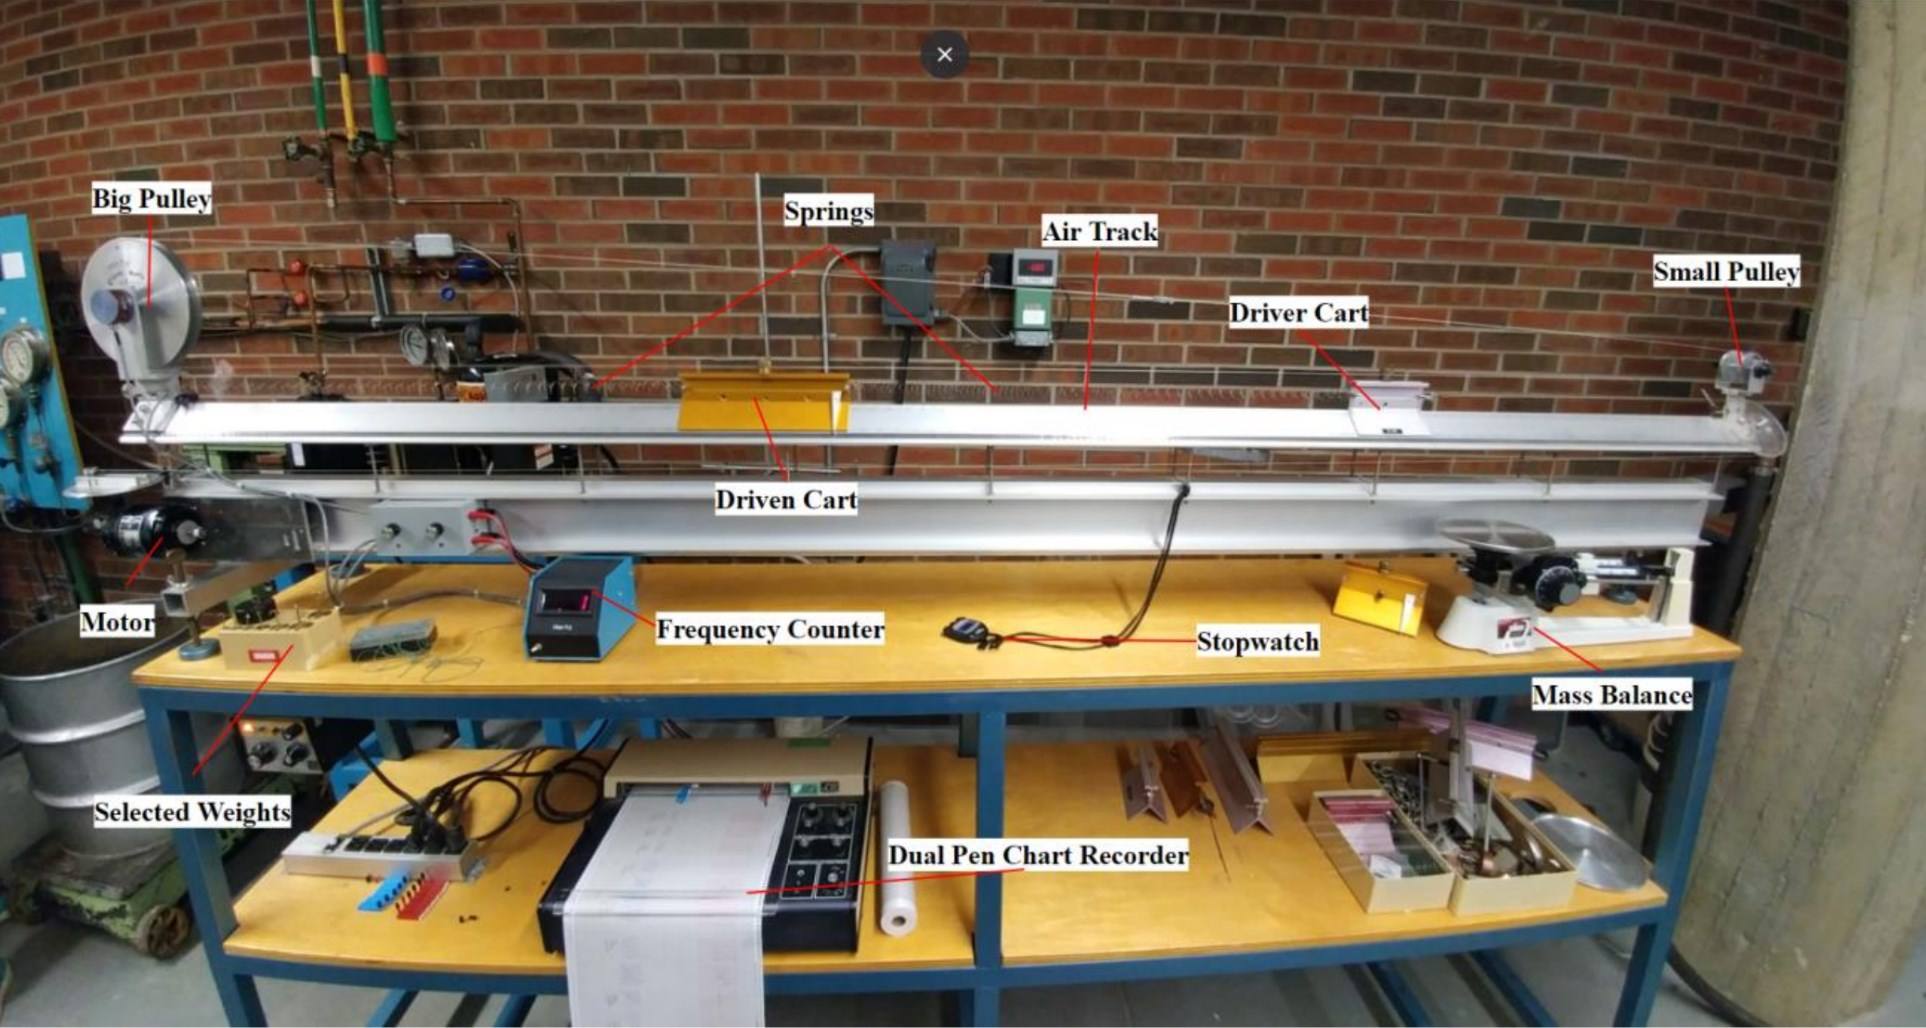
\includegraphics[width=0.5\textwidth]{Sections/Figures/experimental setup.jpg}
    \caption{Experimental Setup of the Spring-Mass System}
\subsection{Equipment}
\begin{itemize}
    \item Air track, to provide a low friction surface for the carts
    \item Two springs, to provide an oscillatory response as the cart is displaced or driven
    \item Frequency counter, to measure the frequency of the forcing motor
    \item A large and small cart, to test the system with different masses
    \item Mass balance, to weigh the carts
    \item Motor and driver cart, to simulate a forced vibration system
    \item Pulleys, to record oscillations using software
    \item Stopwatch, to record the time of 10 oscillations
    \item Chart recorder, to record the oscillations of the system (not used in this experiment, software was used instead)
    \item Weights, to add to the cart to determine the load-deflection relationship of the system
    \item A pan, to hold the weights
\end{itemize}

% Shown above in Figure 1 is the lab apparatus used in this experiment. The air track provides a
% low friction surface (assumed frictionless) for the carts to glide along. The springs attached to the
% cart provide an oscillatory response as the cart is displaced or driven. The frequency counter
% measures this oscillatory response. Two carts of different mass (will be referred to as big and
% small) are tested, and weighed using the mass balance. The weights are added to the cart during
% testing to determine the load-deflection relationship of the system. The motor and driver cart are
% used to simulate a forced vibration system. The measurement system for this involves the
% pulleys, stopwatch, and chart recorder. The pulleys connect to the cart and record oscillations
% using software (note that this was used in place of the chart recorder). Finally, the stopwatch is
% used to record the time of 10 oscillations.

\subsection{Procedure}
\subsubsection{Load Deflection Trial}

\begin{enumerate}
    \item Record the mass of the cart by using the mass balance. Balance the beam by increasing and decreasing the weights on the other side of the beam until the beam is level. The mass of the cart will be used to determine the effective mass of the system for natural frequency calculations.
    \item Set the driving cart to a fixed position (i.e. undriven). This will reduce the system to a single degree of freedom.
    \item Detach the measurement system from the cart. This will allow the cart to oscillate freely.
    \item Turn on the air track to reduce friction between the cart and the track.
    \item Attach the cart to the pan around the free pulley. This will allow the cart to oscillate freely.
    \item Record the initial position of the cart. This will be used to determine the deflection of the cart.
    \item Add a 50 g weight to the pan. Record the new position of the cart. This will be used to determine the deflection of the cart.
    \item Repeat steps 7 and 8, increasing by 50 g until 300 g of weight is reached. This will be used to determine the load-deflection relationship and determine the effective stiffness of the system.
\end{enumerate}

\subsubsection{Free Vibrations}
\begin{enumerate}
    \item Remove the weights from the pan. This will allow the cart to oscillate freely.
    \item Give the cart an ~10cm initial deflection and then release it. This will allow the cart to oscillate freely.
    \item Record the time for the cart to complete ten oscillations using the stopwatch. This will be used to determine the natural frequency of the system.
    \item Repeat steps 2 and 3 five times to get an average value. This will be used to determine the natural frequency of the system.
    \item Redo steps 1-4 for the second, larger cart. This will be used to determine the natural frequency of the system for the larger cart.
\end{enumerate}

\subsubsection{Forced Vibrations}
\begin{enumerate}
    \item Attach the measurement system to the cart. This will allow the software to record the position of the cart.
    \item Attach the driving cart to the motor. This will allow the motor to drive the system.
    \item Turn on the motor and set the frequency below the determined natural frequency. This will allow the system to oscillate at a frequency below the natural frequency.
    \item Once steady state is reached, record the oscillations using the software for about 20 seconds. This will be used to determine the dynamic response of the system.
    \item Repeat steps 3 and 4 for four trials below the natural frequency and four trials above. This will be used to determine the dynamic response of the system.
    \item Redo steps 3-5 for the second, larger cart. This will be used to determine the dynamic response of the system for the larger cart.
\end{enumerate}
\section{Theory}
\subsection{Free Vibrations}
The experimental setup for free vibrations is modelled in Figure \ref{fig:Spring-Mass-Damper System}. The system consists of a mass $m_e$ attached to a spring with stiffness $k_e$. 
\begin{figure}[H]
    \centering
    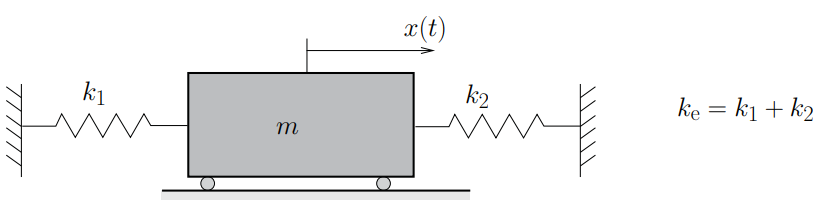
\includegraphics[width=0.5\textwidth]{Sections/Figures/theory spring mass.png}
    \caption{Spring-Mass System}
    \label{fig:Spring-Mass-Damper System}
\end{figure}
If $x$ is the displacement of the mass from its equilibrium position, the equation of motion is given by
\begin{equation}
    m_e\ddot{x} + k_ex = 0 \label{eq:Free Vibration Differential Equation}
\end{equation}
The solution to Equation \ref{eq:Free Vibration Differential Equation} is given by
\begin{equation}
    x(t) = \frac{v_0}{p}\sin(pt) + x_0\cos(pt) \label{eq:Free Vibration Solution}
\end{equation}
where $v_0$ is the initial velocity, $x_0$ is the initial displacement, and $p = \sqrt{\frac{k_e}{m_e}}$ is the natural frequency of the system. The natural frequency is the frequency at which the system will oscillate if it is displaced and released. The period of the system is given by
\begin{equation}
    \tau = \frac{2\pi}{p} \label{eq:Free Vibration Period}
\end{equation}
\subsection{Forced Vibrations}
The experimental setup for forced vibrations is modelled in Figure \ref{fig:Forced Vibrations System Theoretical}. The system consists of a mass $m_e$ attached to a spring with stiffness $k_e$. The force is $F(t) = kY_0\sin(\omega t)$.
\begin{figure}[H]
    \centering
    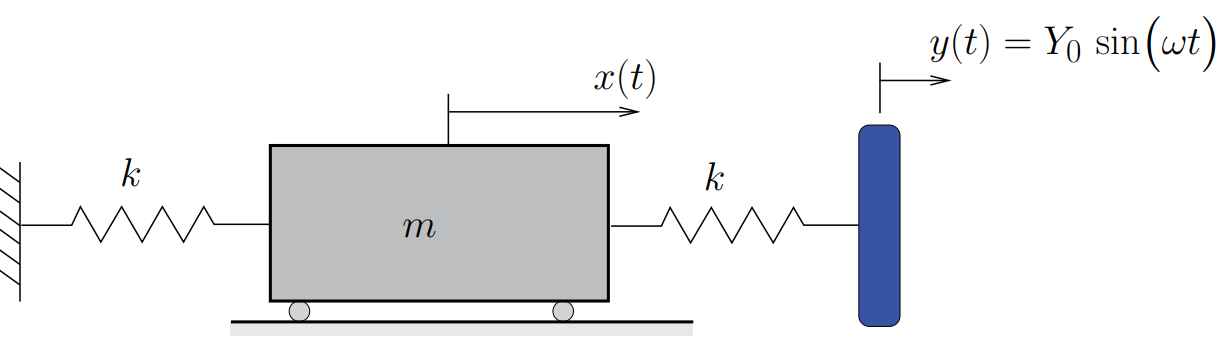
\includegraphics[width=0.5\textwidth]{Sections/Figures/theory forced spring mass.png}
    \caption{Forced Damped Vibrations System}
    \label{fig:Forced Vibrations System Theoretical}
\end{figure}
The equation of motion for the system is given by
\begin{equation}
    m_e\ddot{x} + k_ex = F_0\cos(\omega t) \label{eq:Forced Vibration Differential Equation}
\end{equation}
where $F_0 = kY_0$. The time-dependent solution to Equation \ref{eq:Forced Vibration Differential Equation} is 
\begin{align}
    x(t) &= \frac{Y_0}{2} \left[\frac{1}{1 - \left(\frac{\omega}{p}\right)^2}\right]\sin(\omega t) \label{eq:Forced Vibration Solution} \\
\end{align}
where $p = \sqrt{\frac{k_e}{m_e}}$ is the natural frequency of the system. The DMF is given by
\begin{equation}
    \text{DMF} = \frac{1}{\left|1 - \left(\frac{\omega}{p}\right)^2\right|} \label{eq:DMF}
\end{equation}
Plotting the DMF against $\omega/p$ will give the frequency response of the system, as shown in Figure \ref{fig:DMF}. At $\omega/p< \sqrt{2}$, the DMF $>1$, which means the system amplifies the input force. At $\omega/p > \sqrt{2}$, the DMF $<1$, which means the system attenuates the input force. The system is in resonance at $\omega/p = 1$.
\begin{figure}[h]
    \centering
    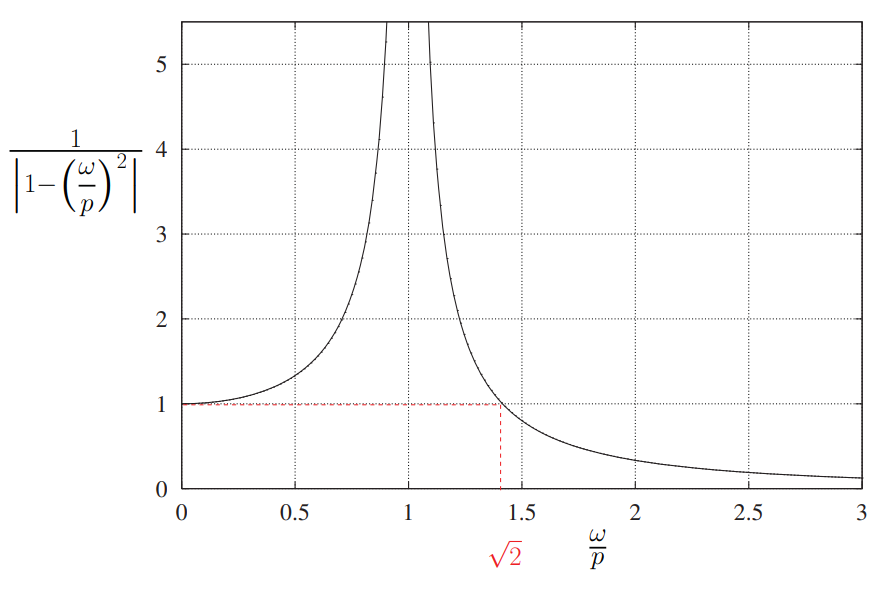
\includegraphics[width=0.5\textwidth]{Sections/Figures/DMF.png}
    \caption{DMF vs. $\omega/p$}
    \label{fig:DMF}
\end{figure}
Defining static deflection as 
\begin{equation}
    \mathbb{X}_0 = \frac{F_0}{k_e} \label{eq:Static Deflection}
\end{equation}
we can see that the $Y_0/2$ term in Eq. \ref{eq:Forced Vibration Solution} is static deflection.

\subsection{Damped Spring Mass System}
\begin{figure}[h]
    \centering
    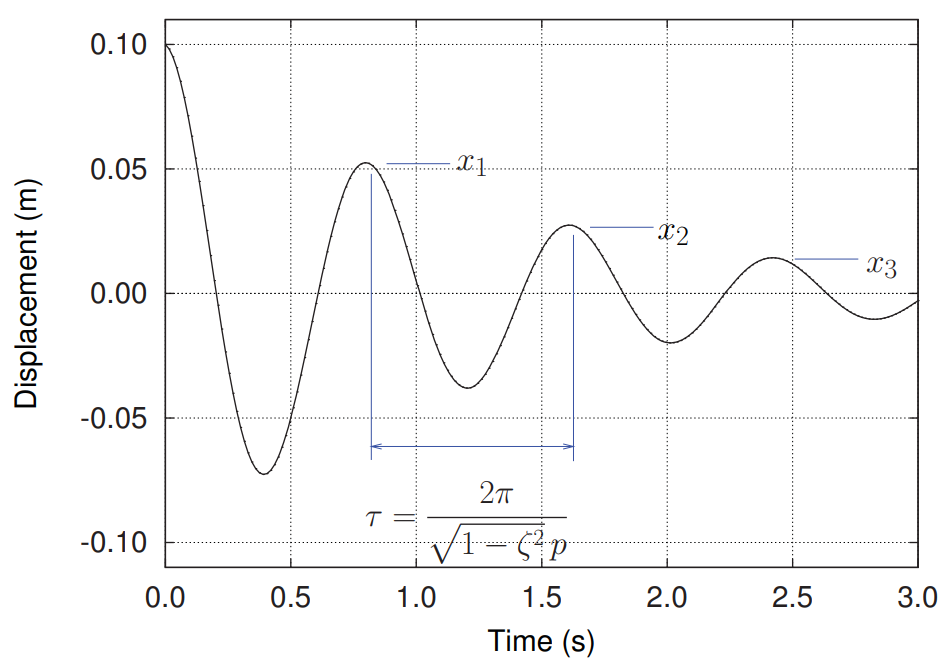
\includegraphics[width=0.5\textwidth]{Sections/Figures/damped response.png}
    \caption{Damped Response of a Spring-Mass System}
    \label{fig:Damped Response}
\end{figure}
An energy dissipation method is added to the system to model the energy loss in the system. The most common approach is to add viscous damping, which is proportional to the velocity of the mass. The equation of motion from Eq. \ref{eq:Free Vibration Differential Equation} is modified to include damping as
\begin{equation}
    m_e\ddot{x} + c_e\dot{x} + k_ex = 0 \label{eq:Damped Vibration Differential Equation}
\end{equation}
where $c_e$ is the damping coefficient. Assuming the mass is given an initial displacement and zero initial velocity, the solution to Eq. \ref{eq:Damped Vibration Differential Equation} is given by
\begin{equation}
    x(t) = A e^{\- \zeta t}\cos\left(\sqrt{1 - \zeta^2}t \right) \label{eq:Damped Vibration Solution}
\end{equation}
where, 
\begin{equation}
    \zeta = \frac{c_e}{2m_e p} = \frac{c_e}{2\sqrt{k_e m_e}} \label{eq:Damping Ratio}
\end{equation}
The solution to Eq. \ref{eq:Damped Vibration Differential Equation} is a decaying sinusoidal function, plotted in Figure \ref{fig:Damped Response}. It can be shown that the peaks can be related by
\begin{align}
    \delta = \ln \left(\frac{x_{n}}{x_{n+1}}\right) = \frac{2\pi}{\sqrt{1 - \zeta^2}} \label{eq:Decay Ratio Delta} 
\end{align}
From which, the damping ratio can be determined as 
\begin{align}
    \zeta = \frac{\delta}{\sqrt{4\pi^2 + \delta^2}} \label{eq:Damping Ratio Calculated With Delta}
\end{align}


\subsection{Equivalent Mass of Measurement System}
\label{sec:Equivalent Mass}
A schematic of the measurement system is shown in Figure \ref{fig:Measurement System}. The equivalent mass of the system is given by
\begin{figure}[H]
    \centering
    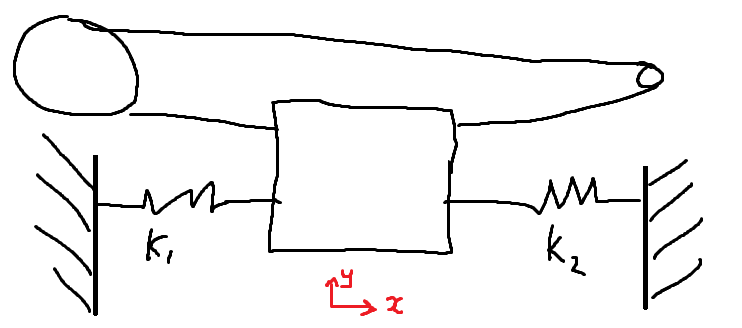
\includegraphics[width=0.5\textwidth]{Sections/Figures/system.png}
    \caption{Cart and Pulley Measurement System}
    \label{fig:Measurement System}
\end{figure}
\begin{figure}[h]
    \centering 
    \begin{minipage}{0.45\textwidth}
        \centering
        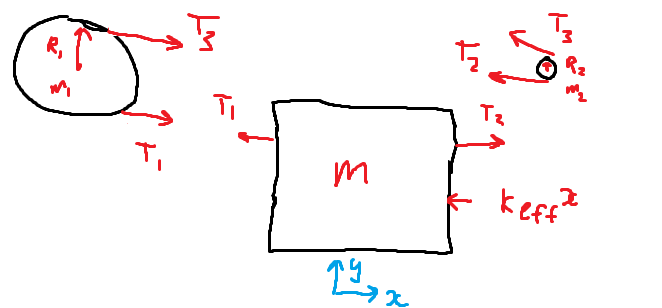
\includegraphics[width=0.9\textwidth]{Sections/Figures/fbd.png}
        \caption{Free Body Diagram of the Cart and Pulleys}
        \label{fig:Cart FBD}
    \end{minipage}\qquad
    \begin{minipage}{0.45\textwidth}
        \centering
        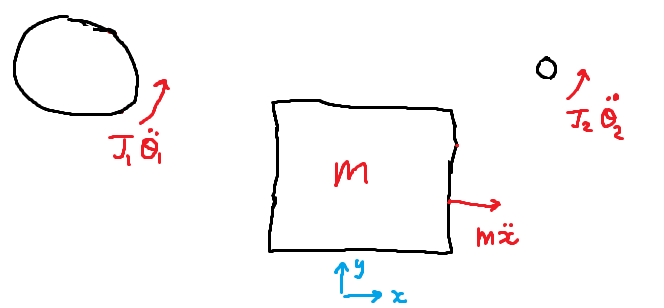
\includegraphics[width=0.9\textwidth]{Sections/Figures/mad.png}
        \caption{Mass Acceleration Diagram of the Cart and Pulleys}
        \label{fig:Cart MAD}
    \end{minipage}  
\end{figure}
Taking the sum of forces in $x$, the moment about pulley 1's and pulley's 2 mass center, 
\begin{align}
    \rightarrow \sum F_x &:= m_{\text{cart}} \ddot{x} \nonumber \\
    &=  T_2 - T_1 - k_{\text{eff}}x \label{eq:Cart Force in x} \\
    \circlearrowleft \sum M_{\text{pulley 1}} &:= J_1 \ddot{\theta}_1 \nonumber \\
    &= R_1 (T_1 - T_3) \label{eq:Pulley 1 Moment} \\
    \circlearrowleft \sum M_{\text{pulley 2}} &:= J_2 \ddot{\theta}_2 \nonumber \\
    &= R_2 (T_3 - T_2) \label{eq:Pulley 2 Moment}
\end{align}
Assuming the cable does not slip,
\begin{align}
    \theta_1 &= \frac{\ddot{x}}{R_1}, \quad \theta_2 = \frac{\ddot{x}}{R_2} \label{eq:Kinematic pure rotation for theta1 and theta2}
\end{align}
Since the disks are uniform disks,
\begin{align}
    J_1 &= \frac{1}{2} m_{1} R_1^2, \quad J_2 = \frac{1}{2} m_{2} R_2^2 \label{eq:Moment of Inertia of Pulleys}
\end{align}
Combining Eq. (\ref{eq:Cart Force in x}), (\ref{eq:Pulley 1 Moment}), (\ref{eq:Pulley 2 Moment}) and using Eq. (\ref{eq:Kinematic pure rotation for theta1 and theta2}) and (\ref{eq:Moment of Inertia of Pulleys}), we get
\begin{align}
    \underbrace{\left(m_{\text{cart}} + \frac{1}{2} m_{1} + \frac{1}{2} m_{2}\right)}_{m_e} \ddot{x} + k_{\text{eff}}x = 0 \label{eq:Equivalent Mass Equation of Motion}
\end{align}
where $m_e$ is the equivalent mass of the system. A full derivation is shown in Appendix \ref{app:Equivalent Mass Derivation}.
\section{Results and Discussion}
\subsection{Main Results}
Table \ref{tab:pump_performance_summary} shows the experimental and manufacturer pump performance summary. The pump configuration, valve configuration, pump speed, volumetric flow rate, corrected head, head coefficient, and flow coefficient are shown. Sample calculations for the single pump in Appendix \ref{sec:single_pump_analysis}. Parallel and series pump performance analysis is shown in Appendix \ref{sec:parallel_and_series_pump_analysis}.
\begin{longtable}{p{0.10\textwidth}p{0.10\textwidth}C{0.08\textwidth}C{0.12\textwidth}C{0.08\textwidth}C{0.12\textwidth}C{0.12\textwidth}}
    \caption{Experimental and Manufacturer Pump Performance Summary} \\
    \label{tab:pump_performance_summary} \\[-8ex]
    \toprule
    Pump Config. & Valve Config. & Pump Speed, $\Omega$ & Volumetric Flow Rate, $Q$ & Corrected Head, $H$ & Head Coefficient, $\Psi$ & Flow Coefficient, $\Phi$ \\
    & & ($\unit{\rpm}$) & ($\unit{\meter\cubed\per\second}$) & ($\unit{\meter}$) & & \\
    \midrule
    Single & Fully open & 1800 & 0.003159 & 2.91 & 0.275 & 0.12 \\
    Single & Partial 1 & 1800 & 0.003003 & 3.16 & 0.300 & 0.11 \\
    Single & Partial 2 & 1800 & 0.001492 & 5.09 & 0.482 & 0.05 \\
    Single & Closed & 1800 & - & 5.49 & 0.520 & 0.00 \\
    Single & Fully open & 2700 & 0.004858 & 5.91 & 0.249 & 0.12 \\
    Single & Partial 1 & 2700 & 0.004749 & 6.31 & 0.265 & 0.12 \\
    Single & Partial 2 & 2700 & 0.002911 & 10.6 & 0.445 & 0.07 \\
    Single & Closed & 2700 & - & 12.4 & 0.522 & 0.00 \\
    Single & Fully open & 3600 & 0.006474 & 9.72 & 0.230 & 0.12 \\
    Single & Partial 1 & 3600 & 0.006240 & 11.2 & 0.266 & 0.11 \\
    Single & Partial 2 & 3600 & 0.002454 & 20.8 & 0.491 & 0.05 \\
    Single & Closed & 3600 & - & 21.8 & 0.515 & 0.00 \\
    Single & Manufacturer & 1800 & 0.0040 & 2.58 & 0.244 & 0.15 \\
    Single & Manufacturer & 1800 & 0.0033 & 4.14 & 0.392 & 0.12 \\
    Single & Manufacturer & 1800 & 0.0026 & 4.96 & 0.470 & 0.10 \\
    Single & Manufacturer & 1800 & 0.0020 & 5.40 & 0.511 & 0.07 \\
    Single & Manufacturer & 2700 & 0.0060 & 5.77 & 0.243 & 0.15 \\
    Single & Manufacturer & 2700 & 0.0050 & 9.12 & 0.384 & 0.12 \\
    Single & Manufacturer & 2700 & 0.0040 & 11.0 & 0.463 & 0.10 \\
    Single & Manufacturer & 2700 & 0.0030 & 12.1 & 0.509 & 0.07 \\
    Single & Manufacturer & 2700 & 0.0020 & 12.8 & 0.539 & 0.05 \\
    Single & Manufacturer & 3600 & 0.0080 & 10.3 & 0.244 & 0.15 \\
    Single & Manufacturer & 3600 & 0.0067 & 16.1 & 0.381 & 0.12 \\
    Single & Manufacturer & 3600 & 0.0054 & 19.2 & 0.454 & 0.10 \\
    Single & Manufacturer & 3600 & 0.0040 & 21.6 & 0.511 & 0.07 \\
    Single & Manufacturer & 3600 & 0.0027 & 22.8 & 0.540 & 0.05 \\
    Parallel & Fully open & 2700 & 0.007266 & 11.3 & 0.474 & 0.18 \\
    Parallel & Partial 1 & 2700 & 0.006283 & 11.7 & 0.492 & 0.15 \\
    Parallel & Partial 2 & 2700 & 0.002217 & 12.5 & 0.528 & 0.05 \\
    Parallel & Closed & 2700 & - & 12.5 & 0.526 & 0.00 \\
    Series & Fully open & 2700 & 0.005584 & 9.15 & 0.385 & 0.14 \\
    Series & Partial 1 & 2700 & 0.005449 & 10.4 & 0.439 & 0.13 \\
    Series & Partial 2 & 2700 & 0.002983 & 21.9 & 0.921 & 0.07 \\
    Series & Closed & 2700 & - & 24.9 & 1.048 & 0.00 \\
    \bottomrule
\end{longtable}

\subsection{Single Pump Performance}
\subsubsection{Head vs. Flow Rate}
Using the data from Table \ref{tab:pump_performance_summary}, the head vs. flow rate for the experimental single pump data was plotted in Figure \ref{fig:single_pump_plot}. Error bars were shown for the volumetric flow, where time was the biggest contributor to error. This is likely due to the reaction time of the stopwatch operator causing a high precision error. The error bars for the head were much smaller and omitted for visual clarity. Calculations for the error bars are shown in Appendix \ref{sec:single_pump_analysis}. 
\begin{figure}[]
    \centering
    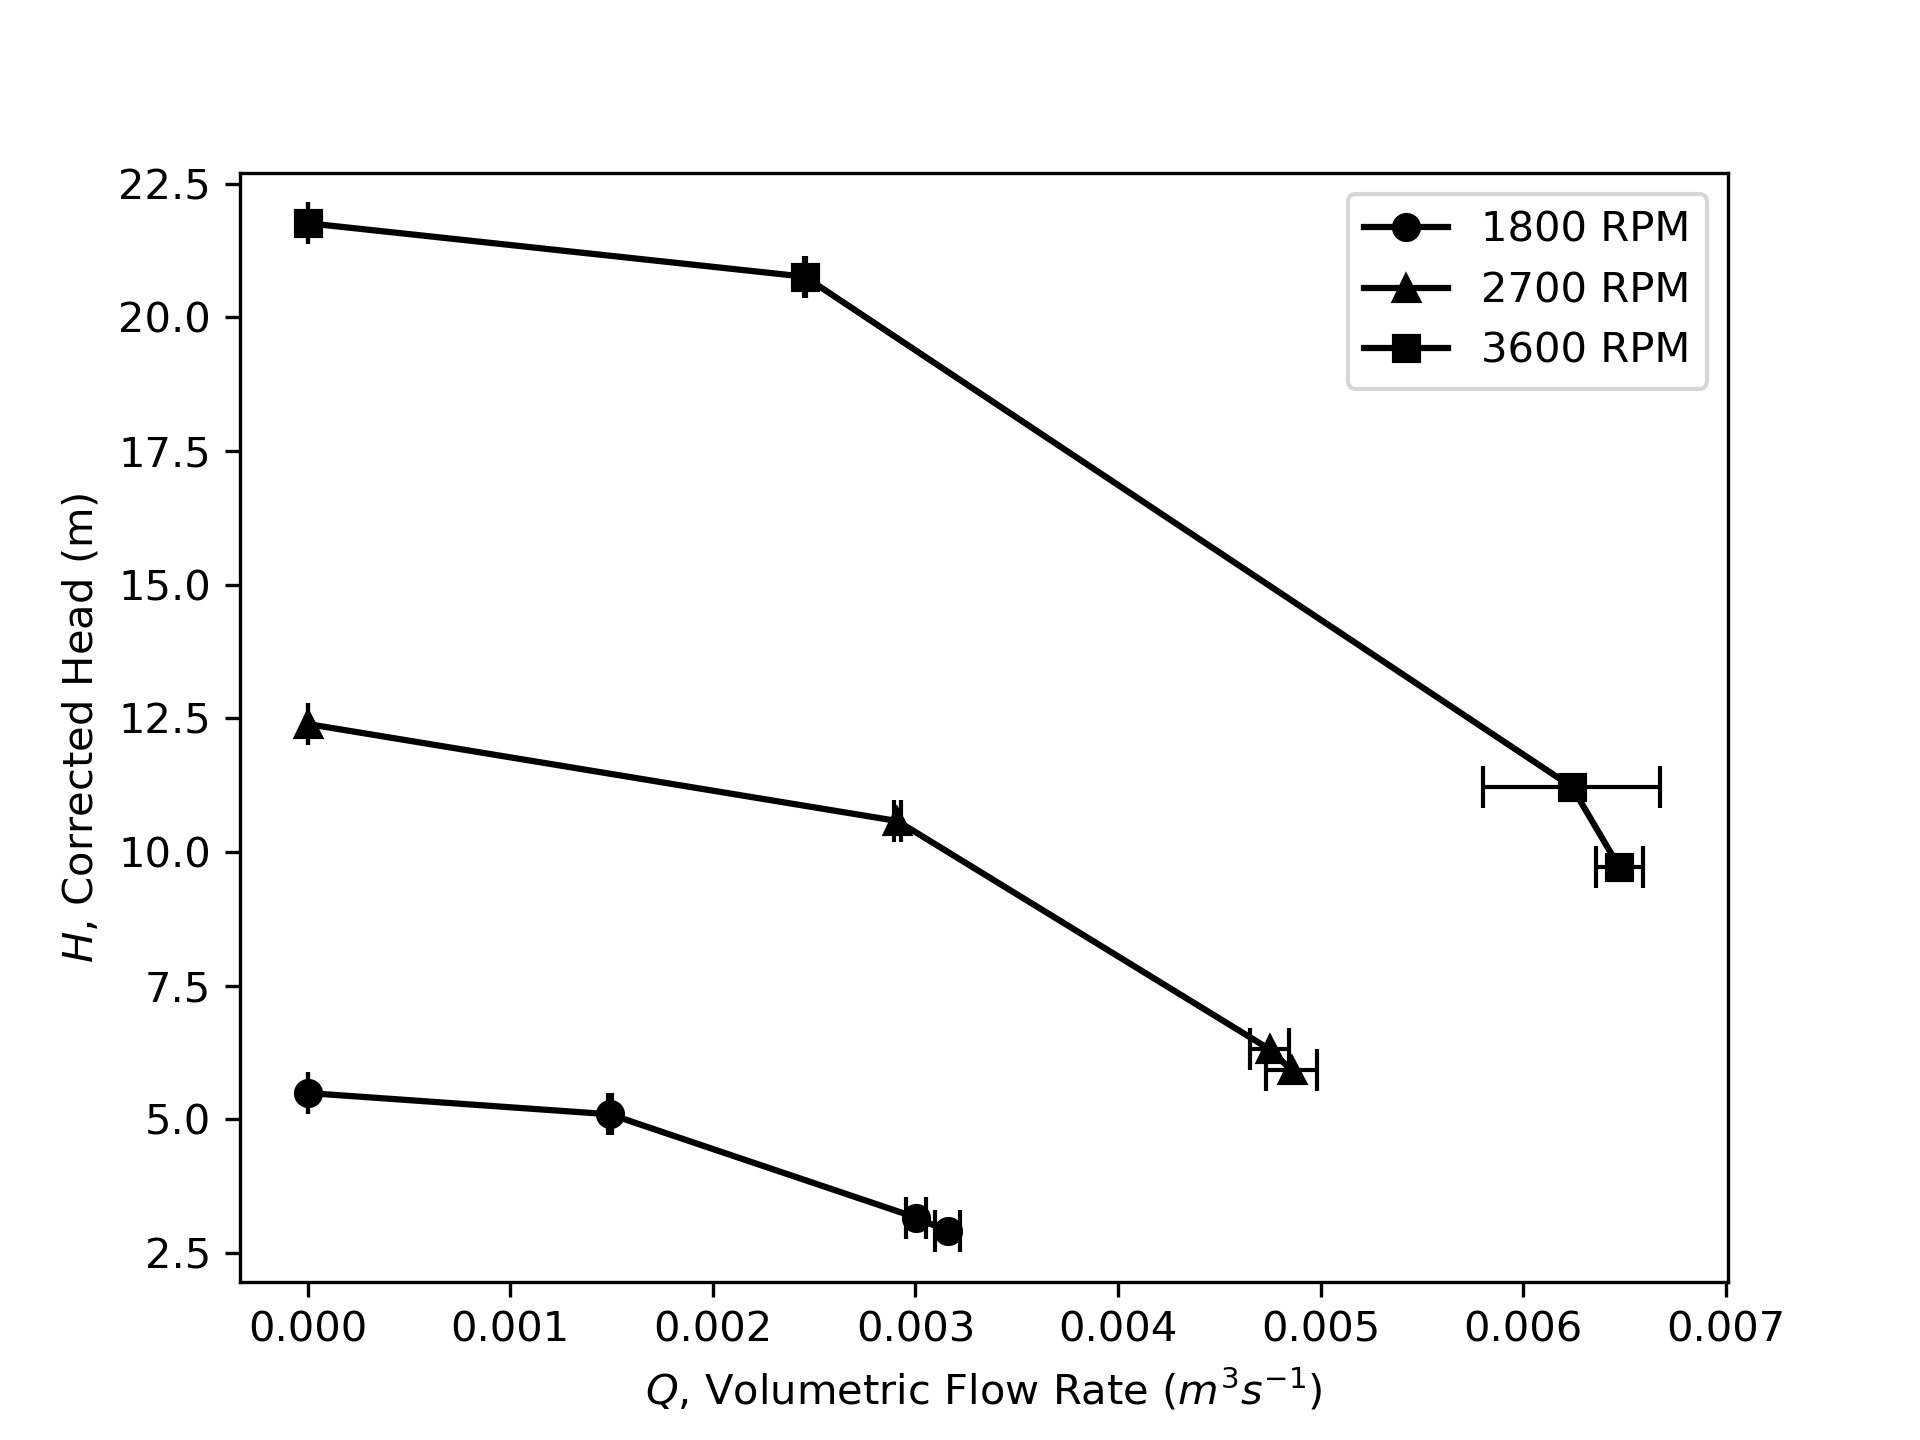
\includegraphics[width=0.5\textwidth]{Sections/Figures/Single Pump Plot.png}
    \caption{Single pump experimental head vs. flow rate plot.}
    \label{fig:single_pump_plot}
\end{figure}

\subsubsection{Head Coefficient vs. Flow Coefficient}
The head coefficient and flow coefficient for the experimental, manufacturer, and ideal pump data are shown in Figure \ref{fig:single_pump_coefficients_plot}. The ideal pump data was calculated from ideal pump equation (Eq. \ref{ideal_turbo_machinary}) using the impeller angle. Impeller angle was determined visually, shown in Appendix \ref{sec:impeller_angle}. Sample calculations for the experimental and manufacturer head and flow coefficients are shown in Appendix \ref{sec:single_pump_analysis}.

For the single experimental pump, the head and flow coefficients appear to fall onto the same curve. A non-linear relationship is observed, where the head coefficient decreases as the flow coefficient increases. Most points of different speeds are within error bars of each other. This suggests that the head and flow coefficients are independent of pump speed. The largest source of error was the precision error caused by the reaction time of the stopwatch operator.

The manufacturer head and flow coefficients also appear to fall onto the same, but different than the experimental, curve. The manufacturer head coefficient is higher than the experimental head coefficient for the same flow coefficient. This suggests that the manufacturer pump is more efficient than the experimental pump. 

The ideal head and flow coefficients are shown as a straight line. The ideal head coefficient is much higher than the experimental and manufacturer head coefficient for the same flow coefficient. The ideal pump neglects all losses and is overly optimistic. The linear trend does not follow the experimental and manufacturer data.
\begin{figure}[]
    \centering
    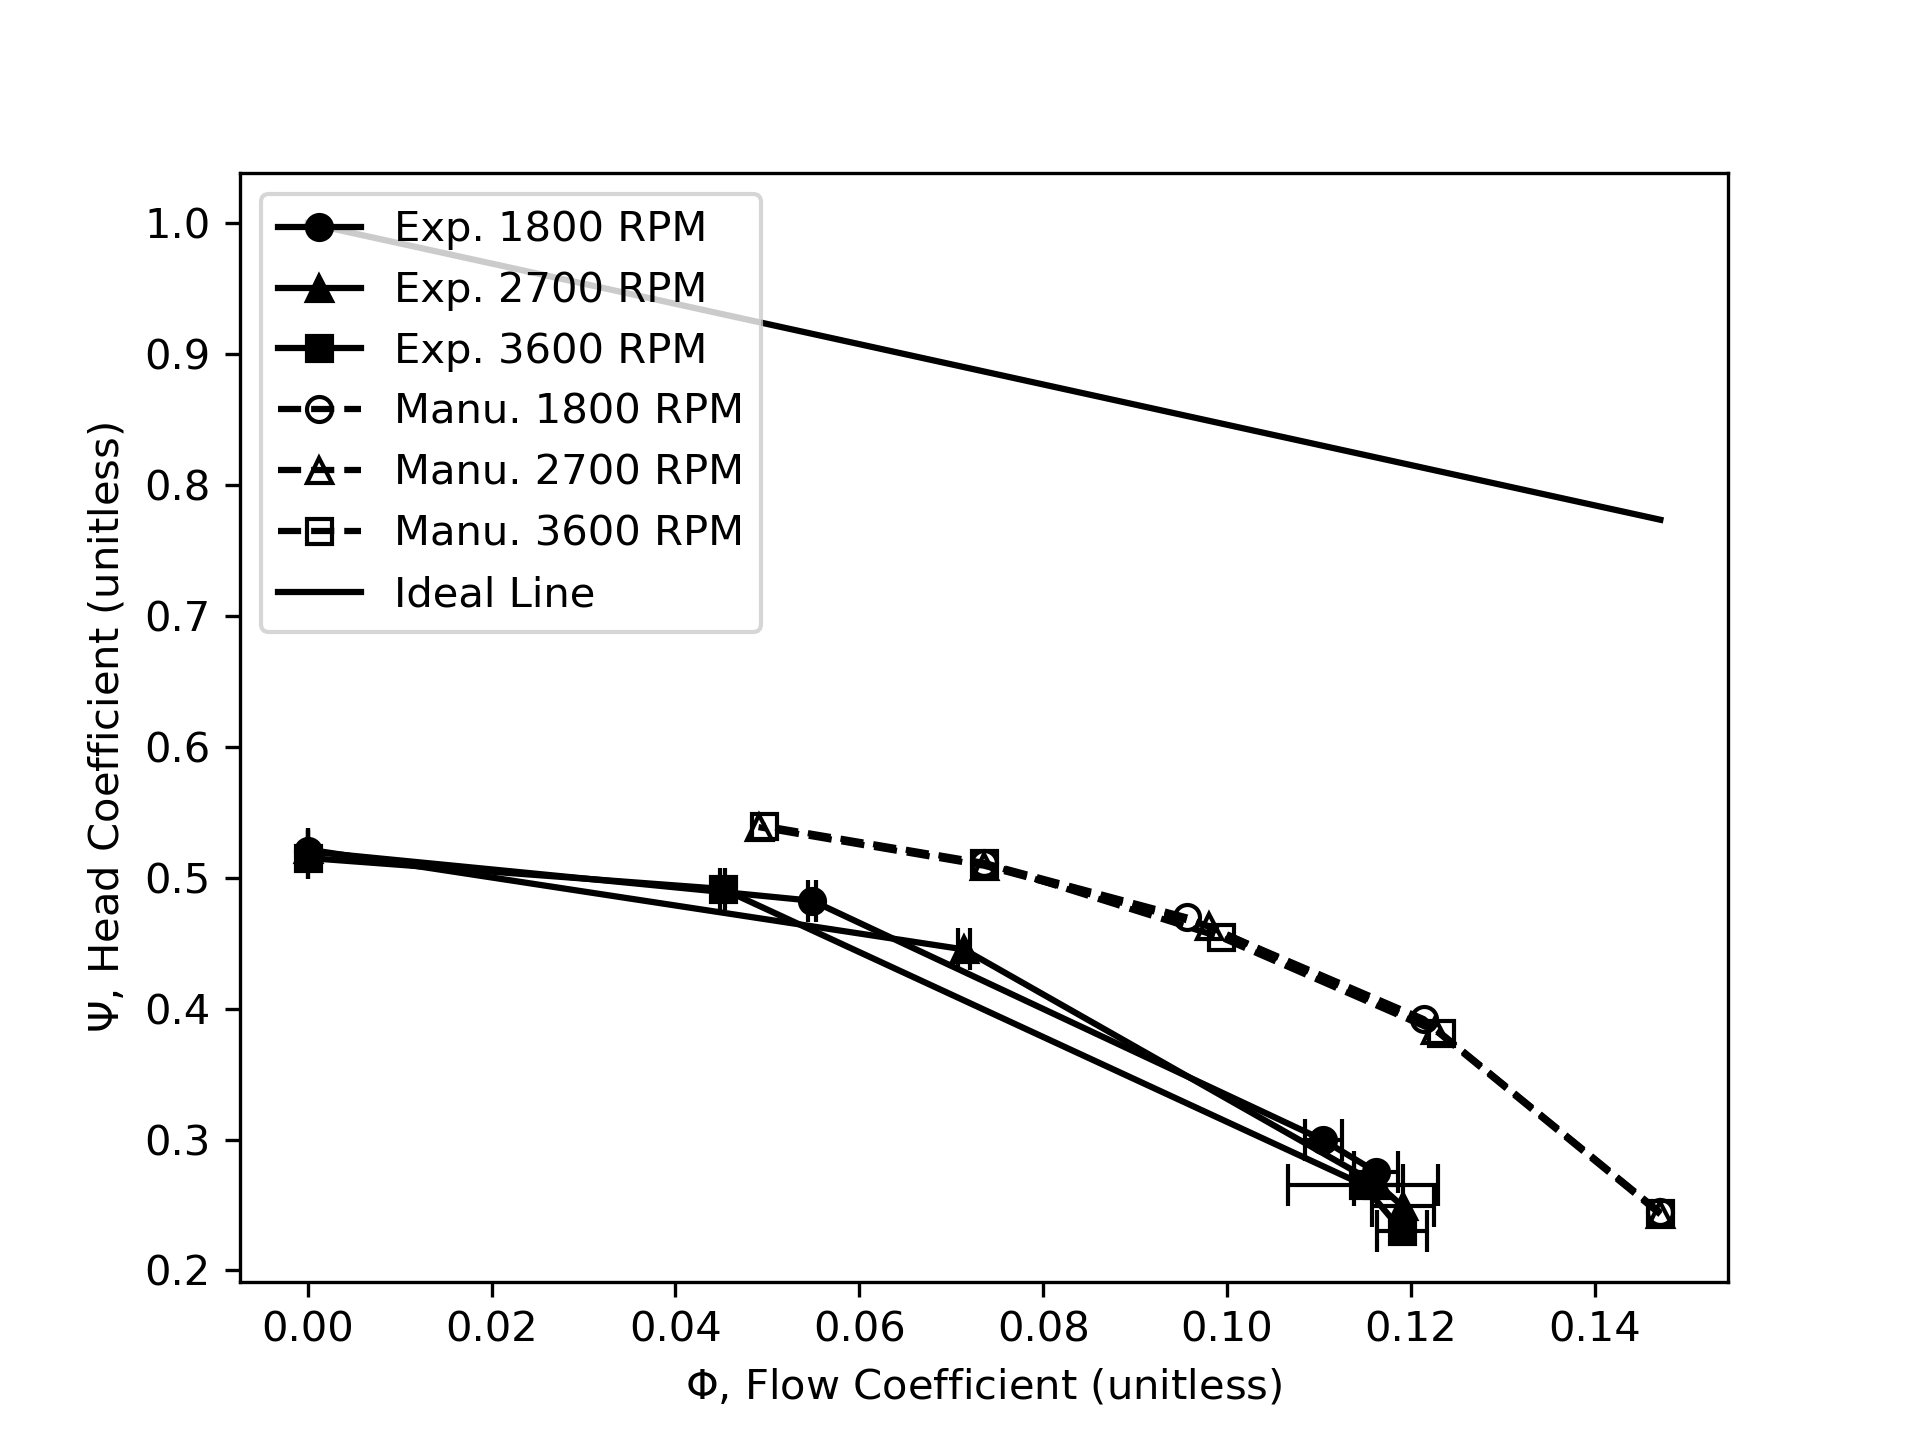
\includegraphics[width=0.6\textwidth]{Sections/Figures/Single Pump Coefficients Plot.png}
    \caption{Single pump experimental, manufacturer, and ideal head coefficient vs. flow coefficient plot.}
    \label{fig:single_pump_coefficients_plot}
\end{figure}

\subsubsection{Ideal and Rule of Thumb Shutoff Head}
\begin{longtable}{C{0.15\textwidth}C{0.15\textwidth}C{0.15\textwidth}}
    \caption{Ideal, rule of thumb, and experimental shutoff head for the single pump at 3600 $\unit{\rpm}$.} \\
    \label{tab:shutoff_head} \\[-8ex]
    \toprule
    Ideal Shutoff Head, $H'_{\text{ideal}}$ & Rule of Thumb Shutoff Head, $H'_{\text{thumb}}$ & Experimental Shutoff Head, $H'_{\text{exp}}$ \\
    ($\unit{\meter}$) & ($\unit{\meter}$) & ($\unit{\meter}$) \\
    \midrule
    42.2 & 21.1 & 21.8 \\
    \bottomrule
\end{longtable}

\noindent The ideal and rule of thumb shutoff head for the single pump at 3600 $\unit{\rpm}$ was calculated and compared to the experimental shutoff head (single closed valve configuration). The ideal and rule of thumb shutoff head was calculated using Eq. \ref{eq:ideal_shutoff_head} and \ref{eq:thumb_head}. The experimental shutoff head was taken from Table \ref{tab:pump_performance_summary}. Sample calculations for the ideal and rule of thumb shutoff head are shown in Appendix \ref{sec:shut_off_head} and the experimental shutoff head in Appendix \ref{sec:single_pump_analysis}.

The ideal shutoff head assumes all kinetic energy is lost too friction and is overly optimistic. The error was calculated to be 48.3\%. This suggests poor agreement between the experimental and ideal shutoff head.

The rule of thumb shutoff head is a more realistic estimate and is within 3.3\% of the experimental shutoff head. This suggests good agreement between the experimental and rule of thumb shutoff head.

\subsection{Parallel Pump Performance}
The head vs. flow rate for the experimental parallel pump data was plotted in Figure \ref{fig:parallel_pump_plot}. Error bars were shown for the volumetric flow, where time was the biggest contributor to error. This is likely due to the reaction time of the stopwatch operator causing a high precision error. The error bars for the head were much smaller and omitted for visual clarity. Calculations for the error bars are shown in Appendix \ref{sec:parallel_and_series_pump_analysis}.

The theoretical curve was calculated using the single pump data. The theoretical head and flow was calculated using Eq. \ref{eq:parallel_head} and \ref{eq:parallel_flow}. The theoretical head and flow was then plotted against the experimental head and flow.

The curves have poor agreement. The theoretical head was higher than the experimental head for the same flow. In addition, a higher flow was observed at the full open valve configuration. This suggests the theoretical model does not accurately predict the parallel pump performance.
\begin{figure}[h]
    \centering
    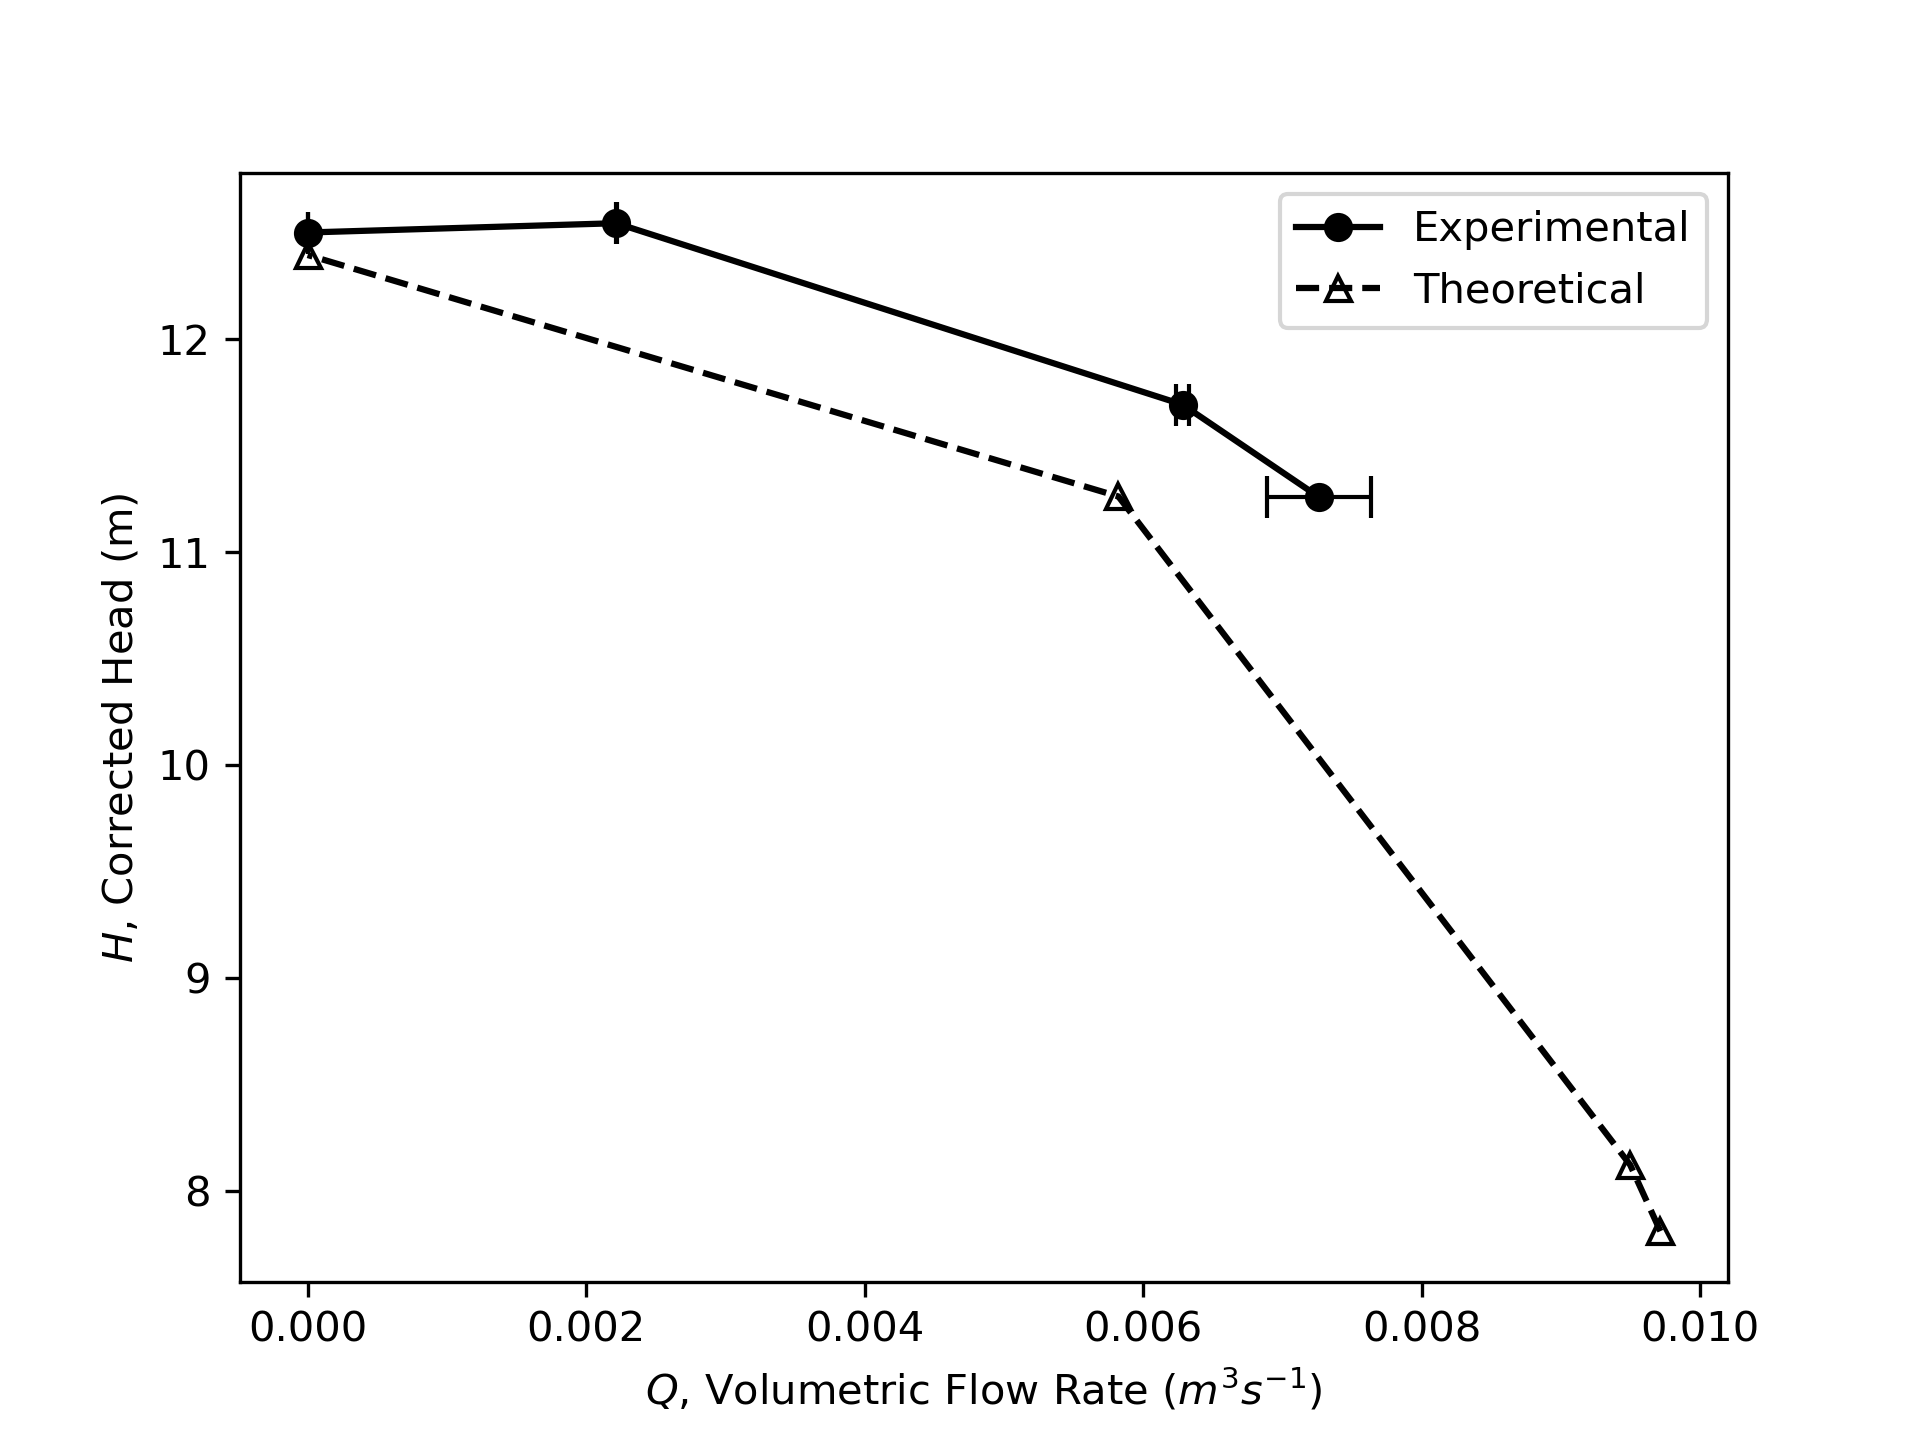
\includegraphics[width=0.5\textwidth]{Sections/Figures/Parallel Pump Plot.png}
    \caption{Parallel pump experimental and theoretical head vs. flow rate plot.}
    \label{fig:parallel_pump_plot}
\end{figure}

\subsection{Series Pump Performance}
The head vs. flow rate for the experimental series pump data was plotted in Figure \ref{fig:series_pump_plot}. Error bars were shown for the volumetric flow, where time was the biggest contributor to error. This is likely due to the reaction time of the stopwatch operator causing a high precision error. The error bars for the head were much smaller and omitted for visual clarity. Calculations for the error bars are shown in Appendix \ref{sec:parallel_and_series_pump_analysis}.

The theoretical curve was calculated using the single pump data. The theoretical head and flow was calculated using Eq. \ref{eq:series_head} and \ref{eq:series_flow}. The theoretical head and flow was then plotted against the experimental head and flow.

The curves have some agreement. The theoretical head was lower than the experimental head for the same flow. In addition, a higher flow was observed at the full open valve configuration. These deviations were smaller than the parallel pump. This suggests the theoretical model does somewhat accurately predicts the series pump performance.

\begin{figure}[h]
    \centering
    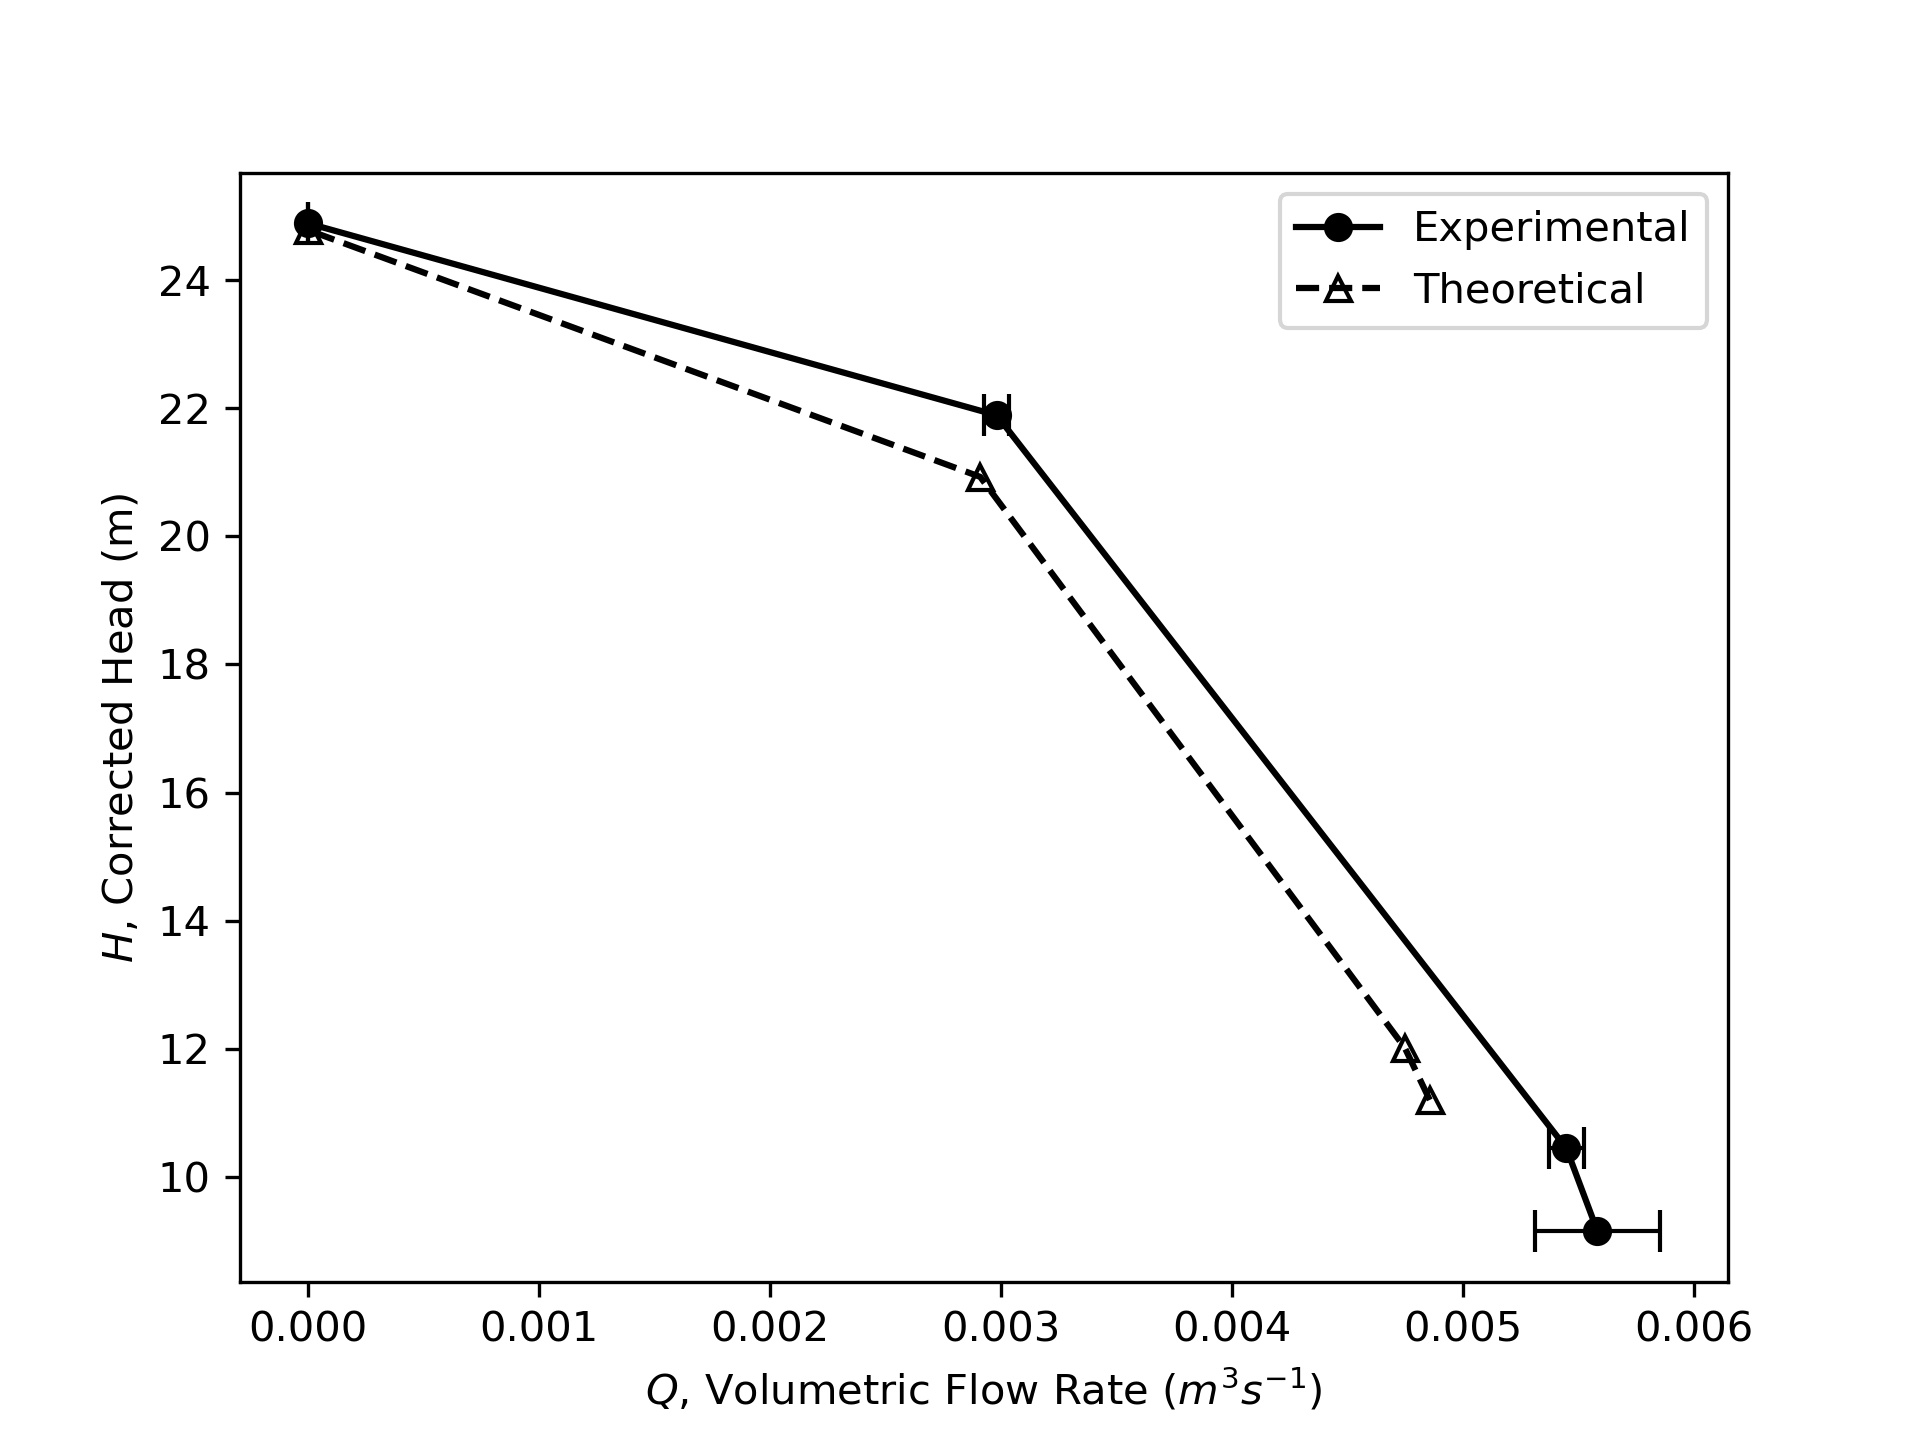
\includegraphics[width=0.5\textwidth]{Sections/Figures/Series Pump Plot.png}
    \caption{Series pump experimental and theoretical head vs. flow rate plot.}
    \label{fig:series_pump_plot}
\end{figure}

\subsection{Geometric Similarity in Manufacturer's Specifications}
The manufacturer's specifications are for geometrically dissimilar pumps. To investigate the effects of assuming similar geometry, two plots were produced. Sample calculations for the head and flow coefficients are shown in Appendix \ref{sec:geometrically_similar_pumps}.

The first plot, Figure \ref{fig:geometric_similarity_head_coefficient}, shows the head coefficient vs. flow coefficient for geometrically similar pumps where impeller blade height, $b$, and impeller width, $w$, were scaled by the impeller diameter, $D$. An observation is that the head coefficient decreases for a given flow coefficient as the impeller diameter decreases.  

The second plot, Figure \ref{fig:geometric_dissimilarity_head_coefficient}, shows the head coefficient vs. flow coefficient for geometrically dissimilar pumps where impeller blade height, $b$, and impeller width, $w$, were not scaled by the impeller diameter, $D$. An observation is that the head coefficient decreases for a given flow coefficient as the impeller diameter decreases. 

The head and flow coefficients for the geometrically similar pumps fall only somewhat collapse onto the same curve. The head and flow coefficients for the geometrically dissimilar pumps fall more so onto the same curve. This suggests that the pumps are geometrically dissimilar, which is consistent with the manufacturer's specifications.
\begin{figure}[h]
    \centering
    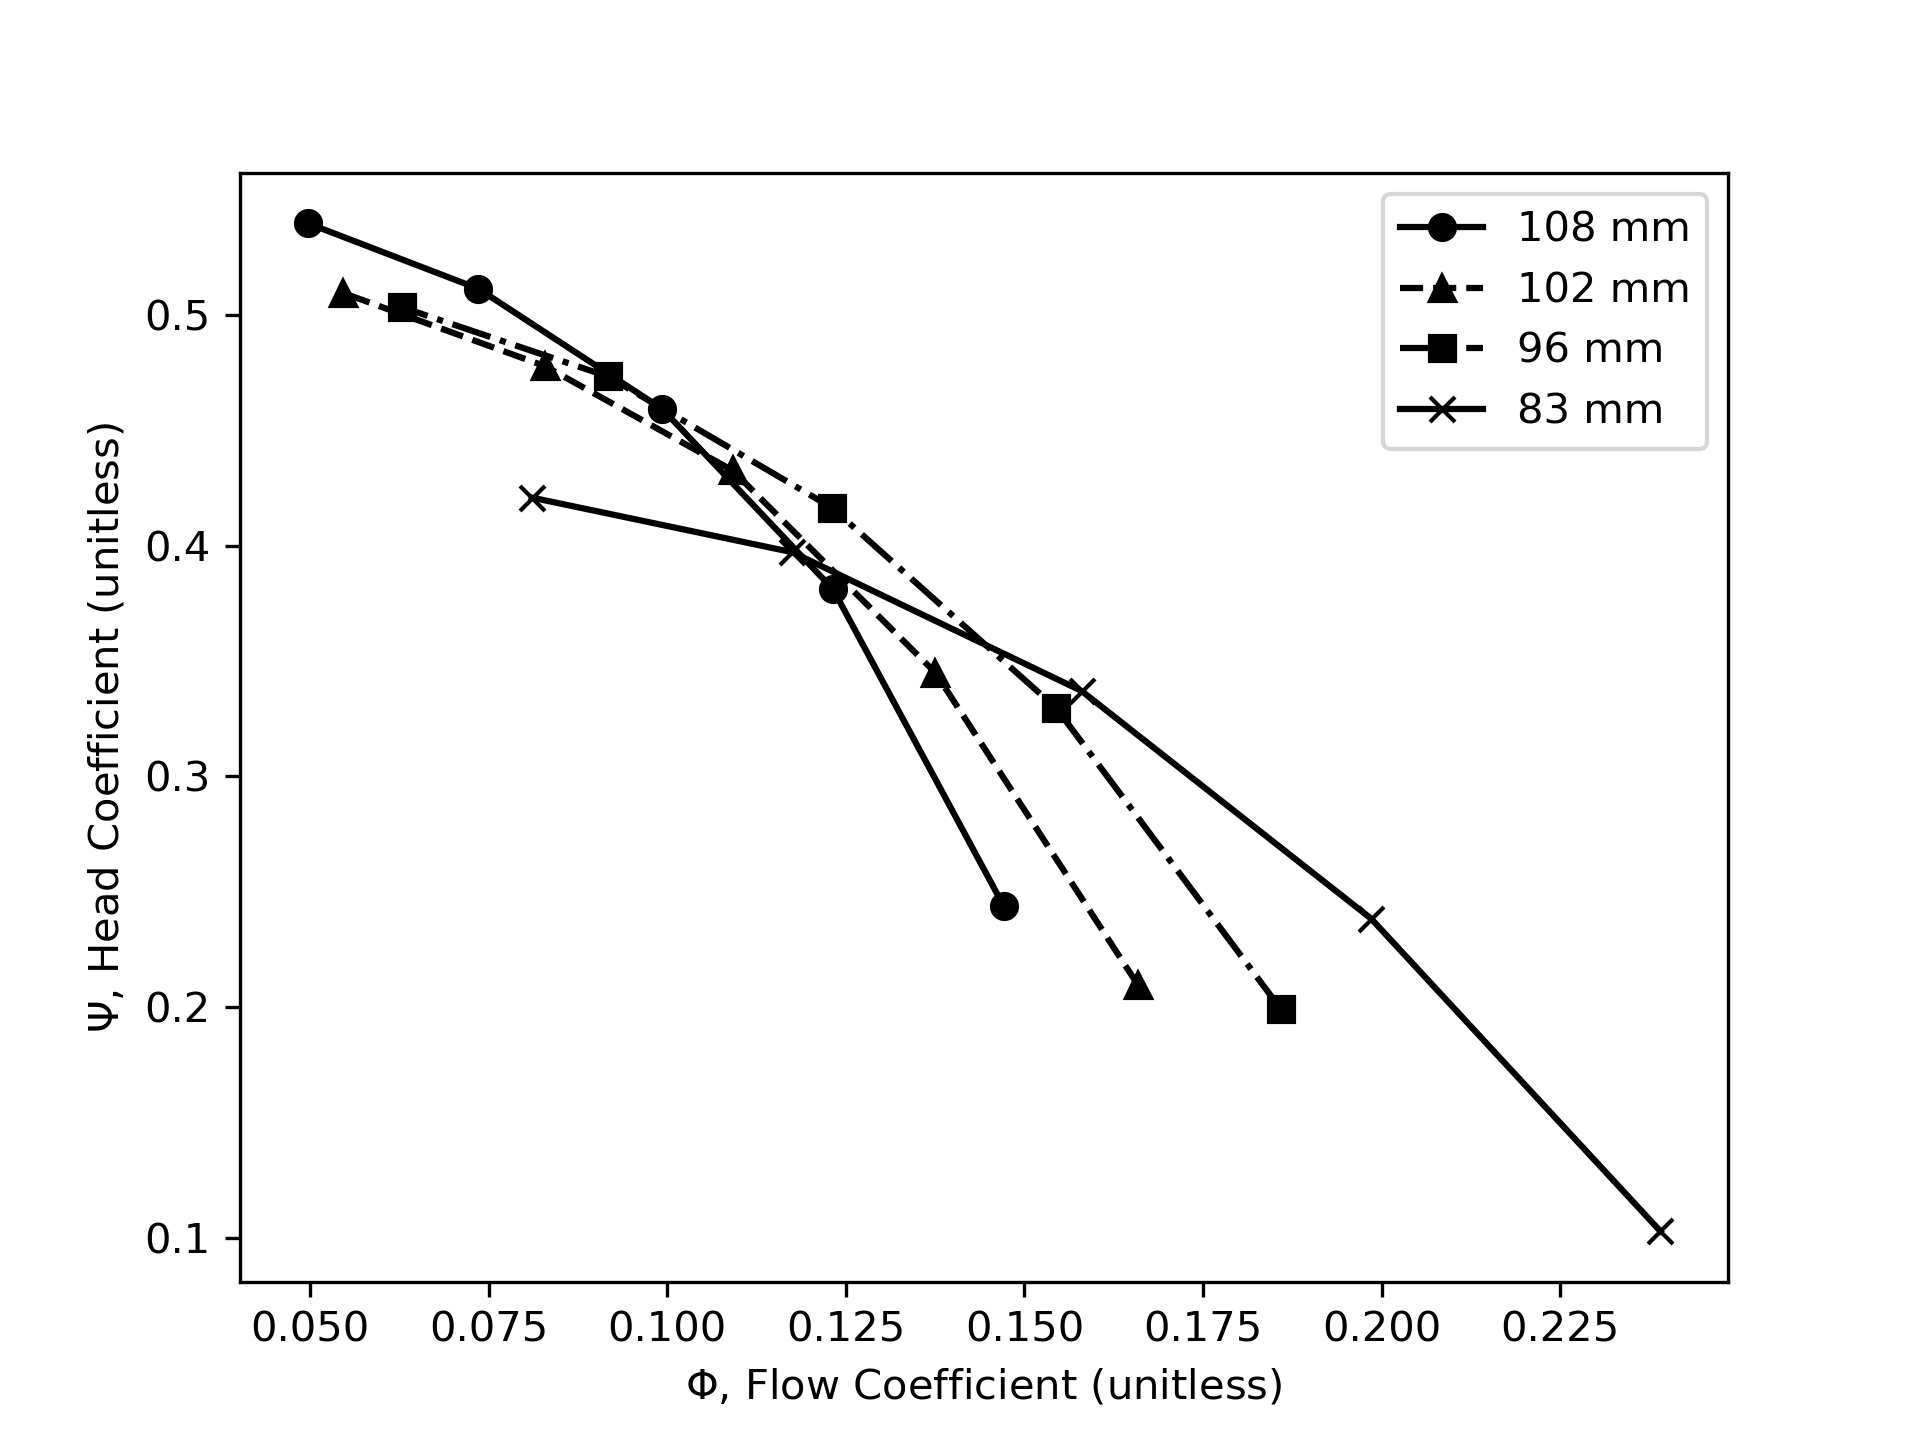
\includegraphics[width=0.5\textwidth]{Sections/Figures/Geometrically Similar Pump Coefficients Plot.png}
    \caption{Head coefficient vs. flow coefficient for geometrically similar pumps.}
    \label{fig:geometric_similarity_head_coefficient}
\end{figure}
\begin{figure}[h]
    \centering
    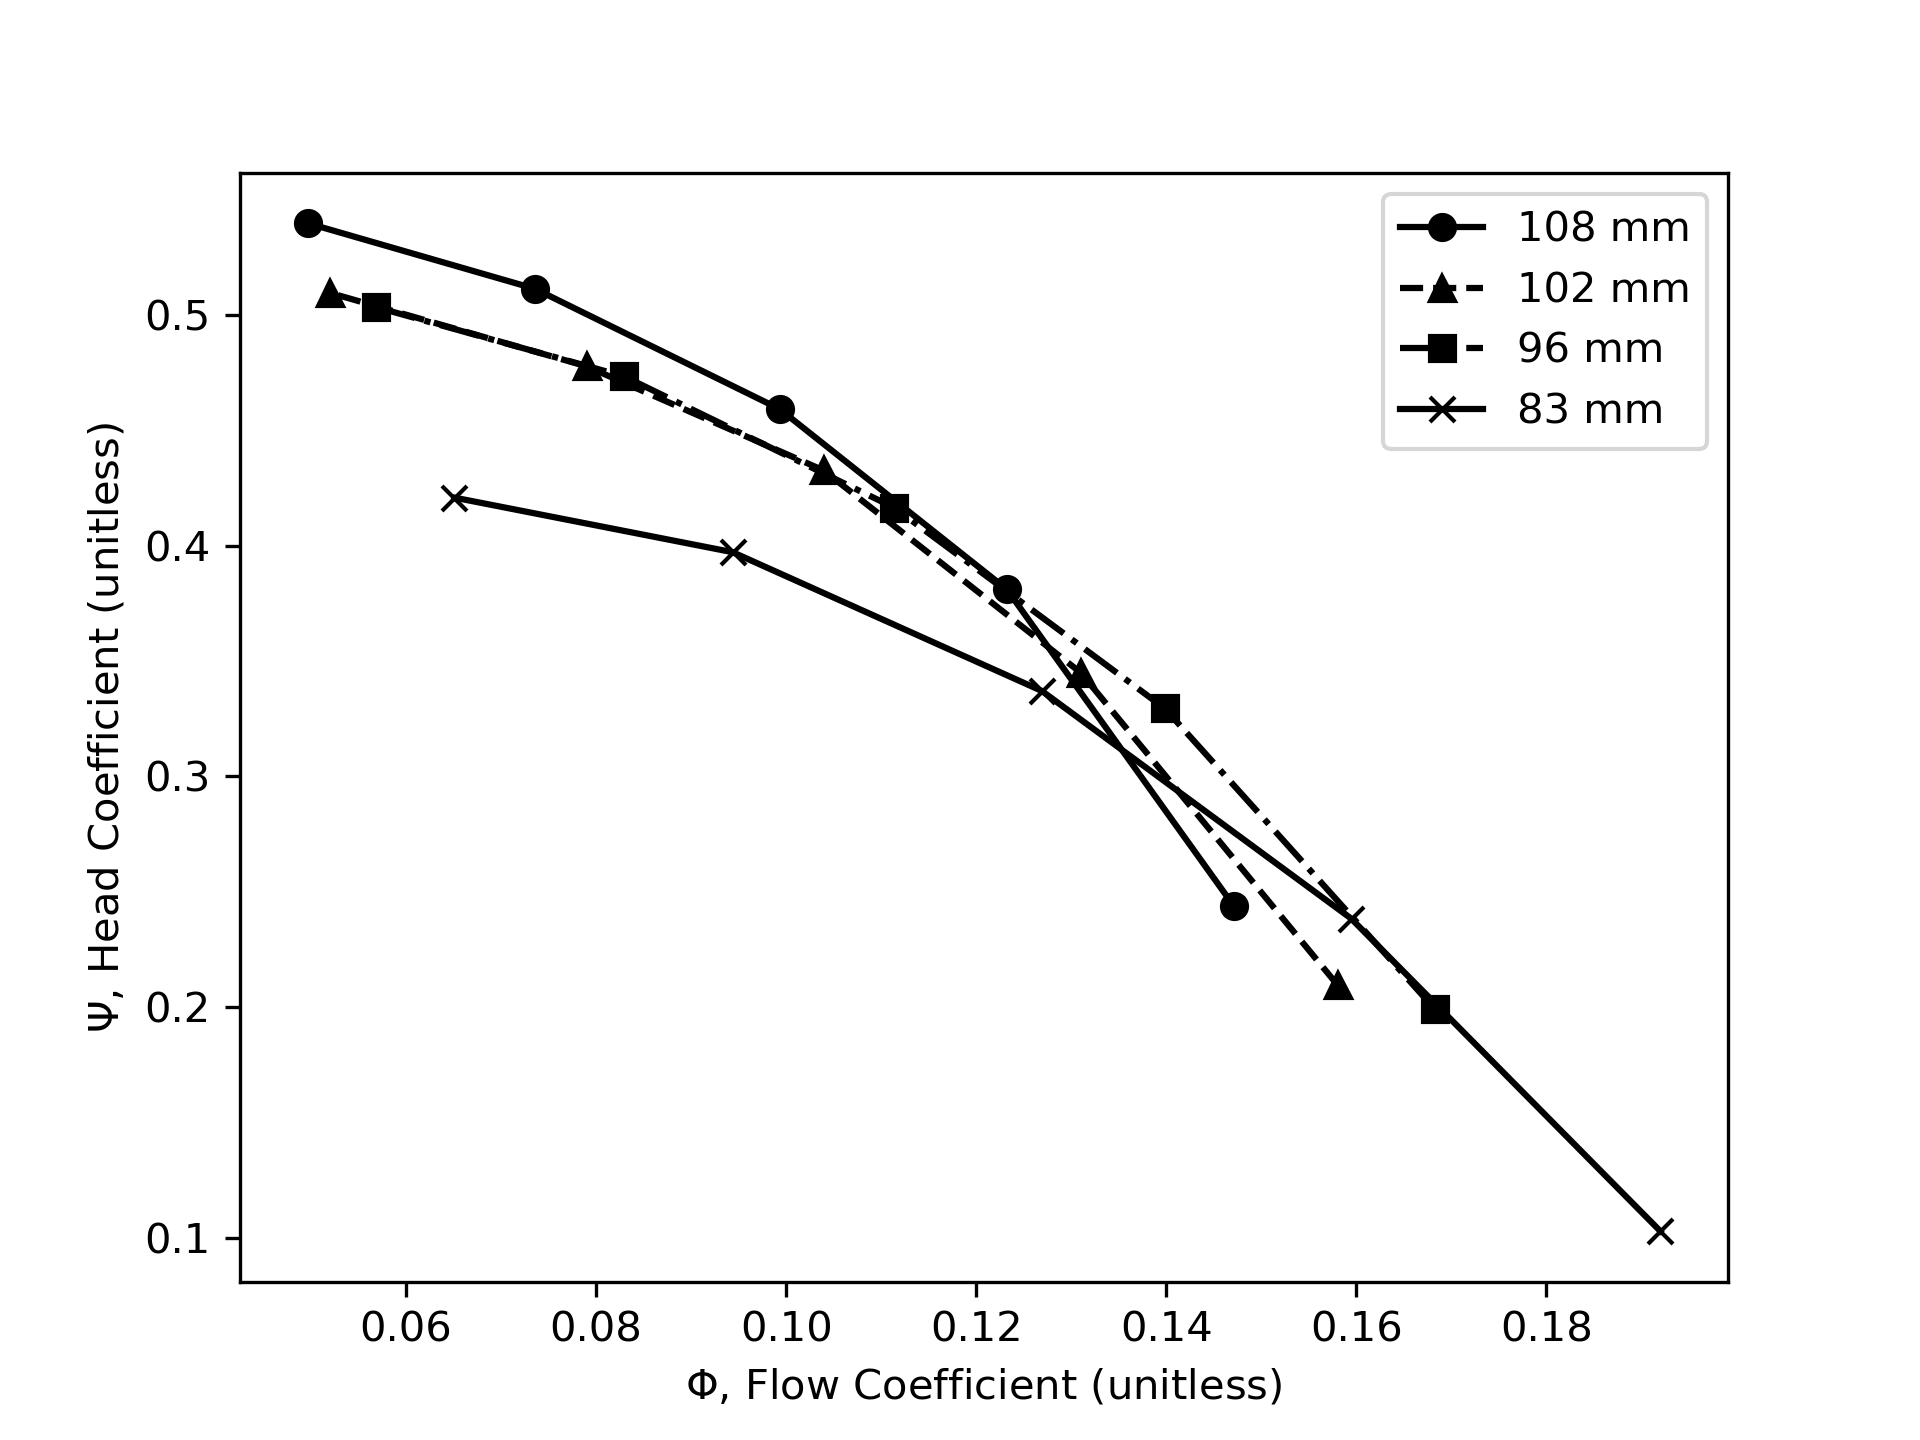
\includegraphics[width=0.5\textwidth]{Sections/Figures/Geometrically Dissimilar Pump Coefficients Plot.png}
    \caption{Head coefficient vs. flow coefficient for geometrically dissimilar pumps.}
    \label{fig:geometric_dissimilarity_head_coefficient}
\end{figure}

\subsection{Pump Efficiency}
The pump efficiencies for the experimental data was calculated in Appendix \ref{sec:todo}. The pump effiecncies for the manufacturer data was given in the manufacturer's specifications. The plot of the experimental and manufacturer pump efficiencies is shown in Figure \ref{fig:single_pump_efficiency_plot}.

The pump was most effiicent when operating at 2700 $\unit{\rpm}$ in a partially closed valve configuration. The pump was least efficient when operating at 1800 $\unit{\rpm}$ in a partially closed valve configuration. 

The actual pump efficiency was lower than the manufacturer pump efficiency for all pump speeds. This could be due to degradation of the pump over time as the setup has been used for many years. 
\begin{figure}[h]
    \centering
    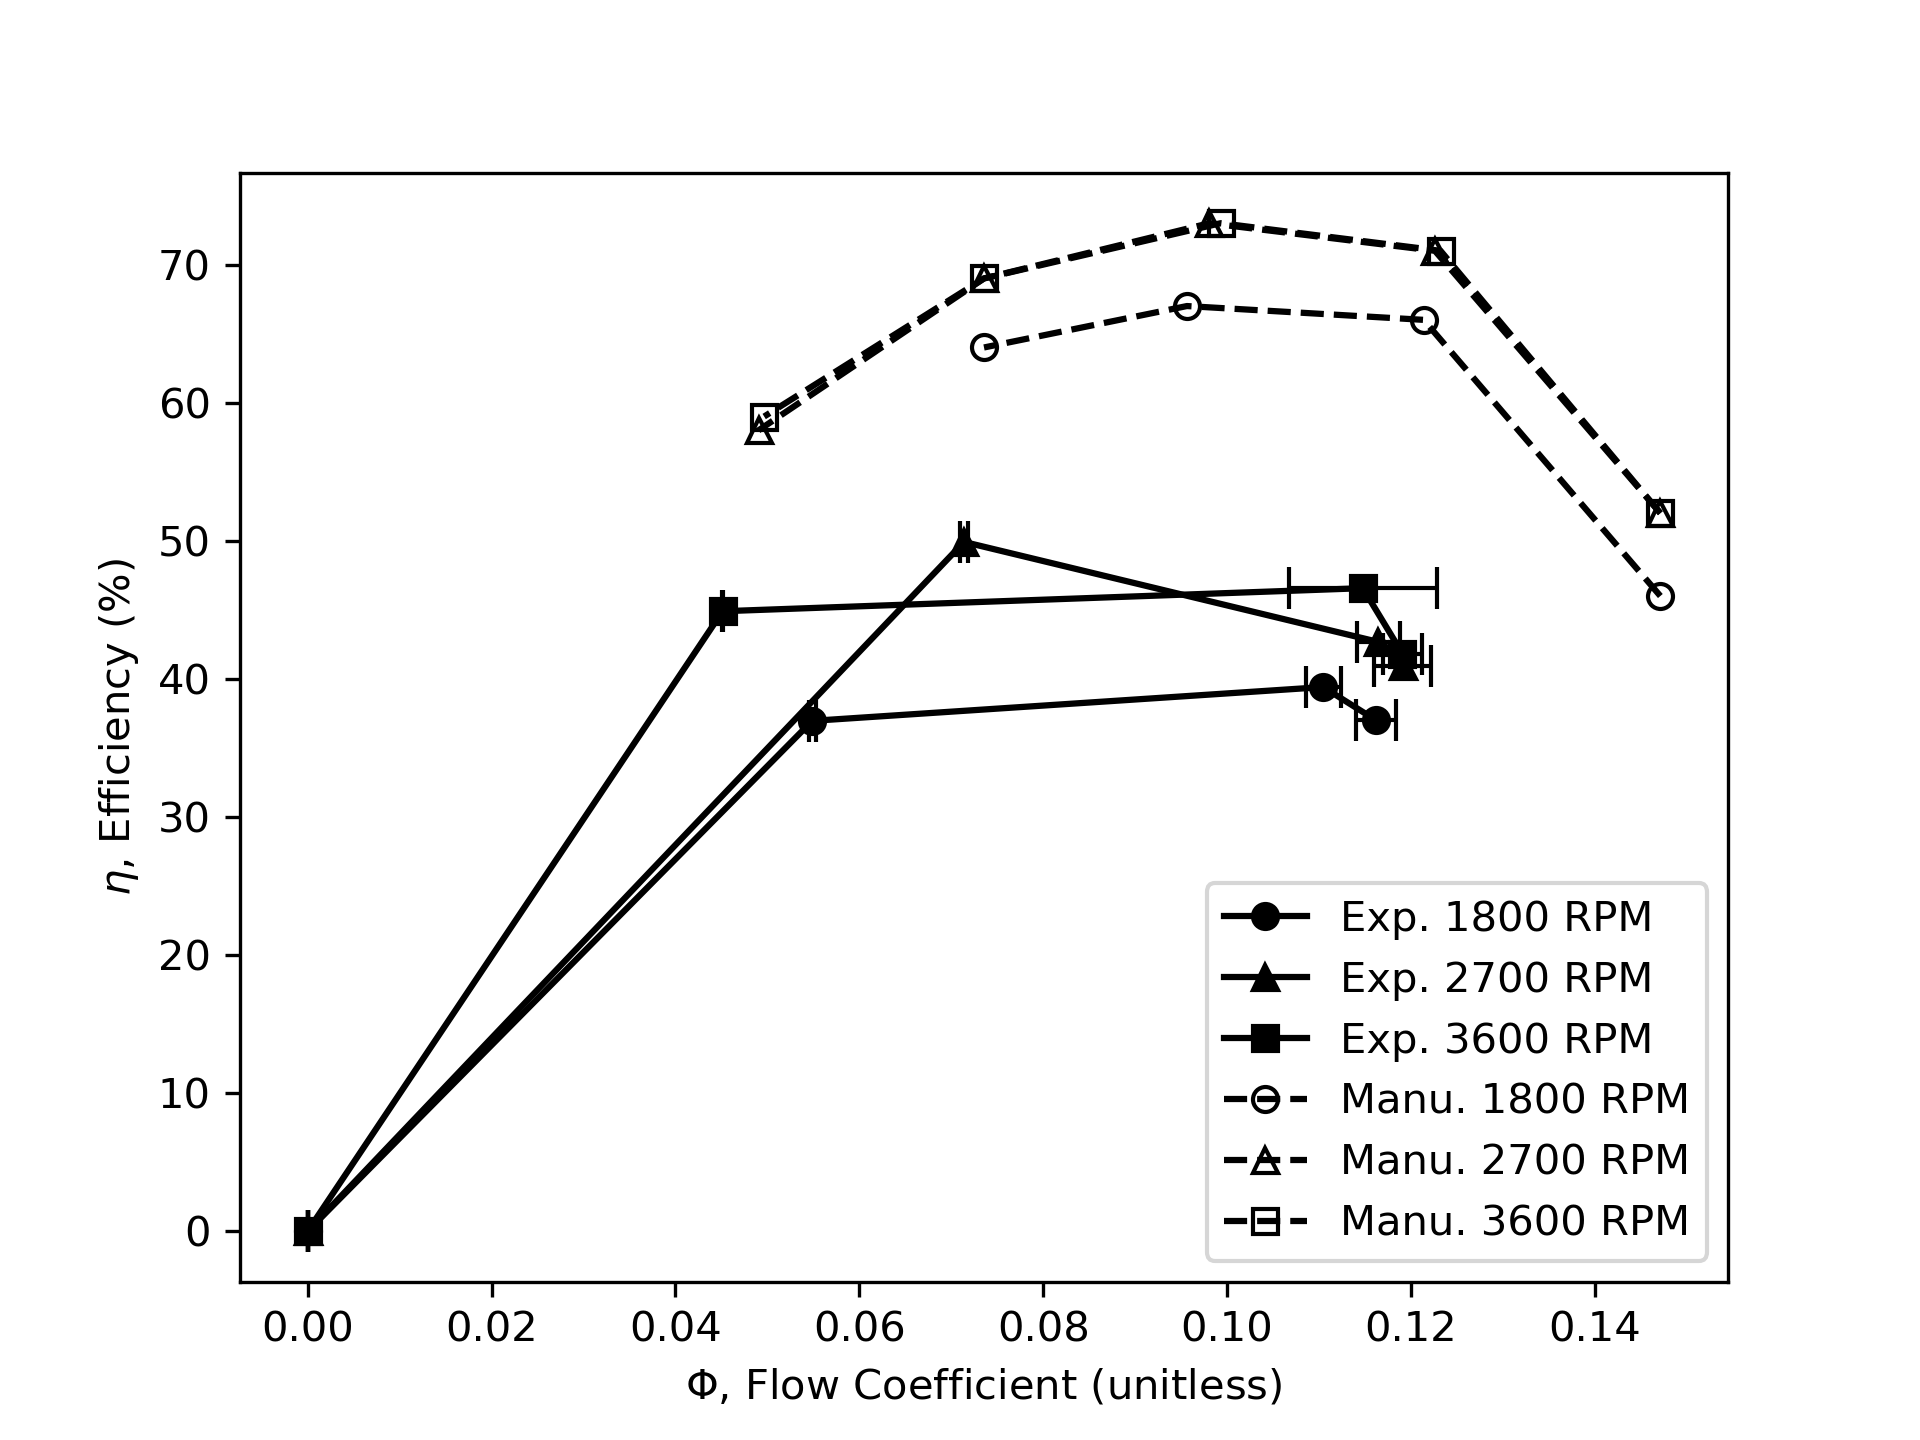
\includegraphics[width=0.5\textwidth]{Sections/Figures/Single Pump Efficiency Plot.png}
    \caption{Single pump experimental and manufacturer efficiency plot.}
    \label{fig:single_pump_efficiency_plot}
\end{figure}

\subsection{Elevation Effects}
The vertical elevation of the pump lines have an effect on the head of the pump. This variation was not accounted for in the modelling. This was because the vertical displacements between where the pressure was measured was small ($< \qty{0.5}{\meter})$. It was assumed that this variation was negligible.
\section{Conclusion}
The modulus of elasticity was determined to be $E = 205 \pm 4.70$ GPa. This quantity was determined from the zero preload trial. The regression used to determine the modulus was $\varepsilon_{b} = 8.47E-05 P$ and had an $R^2 = 0.9992$, indicating a strong linear relationship between the external load and the bolt strain. The preload uncertainty was determined to be $\pm 5\%$ kN from the zero loading trial. The uncertainty is relatively small, which was calculated from the standard error $S_{a}$ of the regression.

The washer calibration was found to be $V_{o, w} = -2.11 \times 10^{-4}P$. This was also calculated from the zero preload trial. This allows prediction of the washer voltage output for a given external load. The regression had an $R^2 = 0.9994$, indicating a strong linear relationship between the external load and the washer transducer.

The torque coefficient was determined to be $0.167$. This was from the zero loading trial, where the torque was varied and the bolt strain was measured. The regression had an $R^2 = 0.9995$, indicating a strong linear relationship between the torque and the preload. The slope value was then used to determine the torque coefficient. This value was within the expected range of $0.1 - 0.2$, adding confidence to the results.

A shakedown test was performed to determine if the bolt was subjected to any torsional loading. The voltage output varied by $\pm 0.005$ V, which was small, the same magnitude as the resolution of the strain transducer. This suggest that the bolt was not subjected to any torsional loading.
T
he uncertainty for the bolt transducer reading was determined from a repeatability test to be $\delta V_{o, b} =\pm 0.03$

The stiffness of the bolt was determined to be $k_b = 209$ MN/m. The bolt was divided into three sections, and the stiffness of each section was determined by modelling the bolt as three distinct sections which act as three springs in series, with stiffness $k_1 = 510$ MN/m, $k_2 = 383$ MN/m, and $k_3 = 4834$ MN/m. 

% don't reference sections
The theoretical and experimental stiffness of the joined members was determined to be $k_m = 2222$ MN/m and $k_m = 1600$ MN/m, respectively. The theoretical stiffness of the joined members was determined by modelling the angle of stress distribution on the member to be 45$^\circ$. The experimental stiffness of the member was determined using the preseparation regression from the static loading no gasket trial. The constant $C$ was determined to be $0.1157$ from the preseparation regression ($R^2 = 0.9983$). The relative error between the theoretical and experimental stiffness of the member was $28.0\%$. The assumption of the stress distribution angle was likely responsible for discrepancies between the theoretical and experimental stiffness of the member. 

During the static loading trials, the gasket decreased the bolt force for a given external load. A separation was observed in the no gasket trial, but not in the gasket trial. This suggest the gasket helped prevent the members from separating. Further testing could be done to determine the separation point of the gasket. The $R^2$ values for the no gasket trial and gasket trial were $0.9983$ and $0.9985$, respectively, indicating a strong linear and quadratic relationship between the external load and the bolt strain. 

The separation point was observed to be $P = 4.98$ kN and $P = 4.67$ kN for the experimental and theoretical values, respectively. The theoretical separation point was determined using the experimental $k_b$ and theoretical $k_m$, whereas the experimental separation point was determined by equating the preseparation and postseparation regressions from the no gasket trial. The relative error between the experimental and theoretical separation points was $6.78\%$. The main discrepancy came from the difference in the experimental and theoretical stiffness of the member, which had a relative error of $28.0\%$.

Both the mean and alternating stresses increased as torque increased. The gasket generally increased the mean stress and alternating stress. The alternating stress decreased as torque increased, and the mean stress increased as torque increased.

The objectives of the lab were achieved: the modulus of elasticity was obtained, the stiffness of the member and bolts were determined, and insights into the effects of torque, preload, external loads, gaskets, and dynamic loading were obtained. The results were consistent with expectations, and the uncertainty was relatively small. The largest sources of error was the uncertainty from the strain transducer, $V_{o, b}$ and the modulus, $E_b$. Future work could be done to verify the stress distribution angle, and to determine the separation point of the gasket.

Understanding these parameters will aid in design and analysis of bolted connections in critical applications. Ensuring safe and reliable operation of bolted connections is essential in many engineering applications, and the results of this lab will be useful in future work.

\section{Technical Recommendations}
One transducer reading for the washer and bolt was measured for a given external load for the zero preload trial. This totaled to nine measurements for the linear regression. Future work could expand by taking three measurements for the washer and bolt transducer for a given external load, which should reduce the standard error of the regression. More thorough calibration of the washer and bolt transducer could be done to reduce the bias uncertainty.

In addition, hysteresis was not accounted for in the zero preload trial, as measurements were only taken upwards. Performing the measurements in both directions could be used to determine the effect of hysteresis on the modulus of elasticity. These recommendations could be used to increase the accuracy and confidence of the modulus of elasticity.

The theoretical value for the stiffness of the member did not match the experimental value, and the effects rippled through the theoretical separation point calculations. The stress distribution angle was assumed to be 45$^\circ$, and was never verified. Future work could be done to verify the stress distribution angle, which could be used to determine the stiffness of the member with higher accuracy and confidence.

The gasket was not tested for separation, and the separation point was not determined. Knowing this could be a critical design parameter. For example, in a boiler, the gasket could be subjected to high temperatures and pressures, and the separation point could be critical to ensure the gasket does not fail. Future work could be done to determine the separation point of the gasket.

The torque wrench was not calibrated, and the uncertainty of the torque wrench was not determined. The torque wrench may be inaccurate, as the operator can go past the click point. Utilizing a digital solution could be more accurate to apply the torque on the bolt.

% \newpage
% \bibliographystyle{IEEEtran}
% \bibliography{citations.bib}
% \bibliography{}

\newpage
\appendix
\renewcommand\thefigure{\thesection.\arabic{figure}}    
\renewcommand\thetable{\thesection.\arabic{table}}
\section{Appendix: Single Pump Analysis}
\label{sec:single_pump_analysis}
This section will discuss the single pump analysis. Experimental discharge, head, head coefficient, and flow coefficient will be calculated and compared to the manufacturer's specifications. The uncertainty in the discharge and head will also be calculated.

\subsection{Single Pump Discharge and Heads}
\begin{table}[H]
    \centering
    \caption{Single pump experimental transducer output and time to collect water for 1800 RPM, 2700 RPM, and 3600 RPM}
    \label{tab:single_pump_transducer_output_and_time}
    \begin{tabular}{lcC{0.15\textwidth}cccC{0.15\textwidth}C{0.15\textwidth}C{0.15\textwidth}C{0.15\textwidth}}
    \toprule
    Configuration & Pump Speed & Transducer Output, $V_{t}$ & \multicolumn{3}{c}{Time to collect water (s)} & Nominal time \\
    \cmidrule(lr){4-6}
    \multicolumn{1}{c}{} & (RPM) & (V) & Trial 1 & Trial 2 & Trial 3 & (s) \\
    \midrule
    Fully open & 1800 & 0.75 & 28.55 & 28.99 & 28.79 & 28.78 \\
    Partial 1 & 1800 & 0.83 & 30.14 & 30.51 & 30.16 & 30.27 \\
    Partial 2 & 1800 & 1.43 & 61.12 & 60.80 & 60.86 & 60.93 \\
    Closed & 1800 & 1.56 & - & - & - & - \\
    Fully open & 2700 & 1.50 & 18.66 & 18.93 & 18.55 & 18.71 \\
    Partial 1 & 2700 & 1.62 & 19.23 & 19.23 & 18.96 & 19.14 \\
    Partial 2 & 2700 & 2.94 & 31.15 & 31.30 & 31.22 & 31.22 \\
    Closed & 2700 & 3.52 & - & - & - & - \\
    Fully open & 3600 & 2.44 & 14.13 & 13.93 & 14.06 & 14.04 \\
    Partial 1 & 3600 & 2.89 & 15.04 & 14.35 & 14.31 & 14.57 \\
    Partial 2 & 3600 & 5.85 & 37.01 & 37.04 & 37.07 & 37.04 \\
    Closed & 3600 & 6.18 & - & - & - & - \\
    \bottomrule
    \end{tabular}%
\end{table}
\begin{table}[H]
    \centering
    \caption{Single pump experimental discharge and heads for 1800 RPM, 2700 RPM, and 3600 RPM}
    \label{tab:single_pump_discharge_and_heads}
    \begin{tabular}{lcC{0.15\textwidth}C{0.15\textwidth}C{0.15\textwidth}}
    \toprule
    Configuration & Pump Speed & Volume Flow, $Q$ & Transducer Head, $H_t$ & Corrected Head, $H$ \\
    & (RPM) & ($\unit{\meter\cubed\per\second}$) & (m) & (m) \\
    \midrule
    Fully open & 1800 & 0.003159 & 2.64 & 2.91 \\
    Partial 1 & 1800 & 0.003003 & 2.92 & 3.16 \\
    Partial 2 & 1800 & 0.001492 & 5.04 & 5.09 \\
    Closed & 1800 & - & 5.49 & 5.49 \\
    Fully open & 2700 & 0.004858 & 5.28 & 5.91 \\
    Partial 1 & 2700 & 0.004749 & 5.70 & 6.31 \\
    Partial 2 & 2700 & 0.002911 & 10.4 & 10.6 \\
    Closed & 2700 & - & 12.4 & 12.4 \\
    Fully open & 3600 & 0.006474 & 8.59 & 9.72 \\
    Partial 1 & 3600 & 0.006240 & 10.2 & 11.2 \\
    Partial 2 & 3600 & 0.002454 & 20.6 & 20.8 \\
    Closed & 3600 & - & 21.8 & 21.8 \\
    \bottomrule
    \end{tabular}
\end{table}
\noindent Sample calculations are evaluated for the fully open configuration at 1800 RPM. Starting with time,
\begin{align*}
        t &= \frac{\sum t_i}{n} = \frac{\qty{28.55}{\second} + \qty{28.99}{\second} + \qty{28.79}{\second}}{3} = \qty{28.78}{\second}
\end{align*}
The volumetric flow rate was calculated using water which had a mass of $m = \qty{200}{\lb} = \qty{90.7}{\kilo\gram}$ and a density of $\rho = \qty{998}{\kilo\gram\per\meter\cubed}$. Then,
\begin{align*}
    Q &= \frac{m}{\rho t} = \frac{\qty{90.7}{\kilo\gram}}{\qty{998}{\kilo\gram\per\meter\cubed} \times \qty{28.78}{\second}} = \qty{0.003159}{\meter\cubed\per\second}
\end{align*}
The transducer head was found by
\begin{align*}
    H_t &= \frac{\Delta P}{\rho g} = \frac{\qty{0.75}{\volt} \times \qty{5}{\psi\per\volt} \times \qty{6894.76}{\pascal\per\psi}}{\qty{998}{\kilo\gram\per\meter\cubed} \times \qty{9.81}{\meter\per\second\squared}} = \qty{2.64}{\meter}
\end{align*}
The corrected head was found using inlet diameter, $D_1 = \qty{0.0508}{\meter}$, and outlet diameter, $D_2 = \qty{0.0381}{\meter}$, by
\begin{align*}
    H &= H_t + \frac{8Q^2}{\pi^2 D_2^4 g} \left[1 - \left(\frac{D_2}{D_1}\right)^4\ \right] \\
    &= \qty{2.64}{\meter} + \frac{8 \times (\qty{0.003159}{\meter\cubed\per\second})^2}{\pi^2 \times (\qty{0.0381}{\meter})^4 \times \qty{9.81}{\meter\per\second\squared}} \left[1 - \left(\frac{\qty{0.0381}{\meter}}{\qty{0.0508}{\meter}}\right)^4\ \right] \\
    &= \qty{2.91}{\meter}
\end{align*}

\subsubsection{Single Pump Discharge and Head Uncertainty}
% split table into two tables
% \begin{table}[h]
%     \centering
%     \caption{Single pump experimental discharge and head uncertainties for 1800 RPM, 2700 RPM, and 3600 RPM}
%     \label{tab:single_pump_discharge_and_head_uncertainty}
%     \resizebox{\textwidth}{!}{
%     \begin{tabular}{lC{0.15\textwidth}C{0.10\textwidth}C{0.12\textwidth}C{0.08\textwidth}C{0.10\textwidth}C{0.10\textwidth}C{0.10\textwidth}C{0.15\textwidth}C{0.10\textwidth}}
%         \toprule
%         Valve Configuration & Pump Speed & Time STDEV, $S_{t}$ & Time Precision, $P_t$ & Time Bias, $B_t$ & Time Uncertainty, $\delta_t$ & Flow Uncertainty, $\delta_Q$ & Transducer Uncertainty, $\delta_{V_{\text{tr}}}$ & Head Uncertainty, $\delta_{H_t}$ & Corrected Head Uncertainty, $\delta_{H}$ \\
%         & (RPM) & (s) & ($\pm$s) & ($\pm$s) & ($\pm$s) & ($\pm\unit{\meter\cubed\per\second}$) & ($\pm$V) & ($\pm$m) & ($\pm$m) \\
%         \midrule
%         Fully open & 1800 & 0.2203 & 0.5473 & 0.20 & 0.58 & 6.40E-05 & 0.01 & 0.04 & 0.04 \\
%         Partial 1 & 1800 & 0.2081 & 0.5169 & 0.20 & 0.55 & 5.50E-05 & 0.01 & 0.04 & 0.04 \\
%         Partial 2 & 1800 & 0.1701 & 0.4225 & 0.20 & 0.47 & 1.14E-05 & 0.01 & 0.04 & 0.04 \\
%         Closed & 1800 & - & - & - & - & - & 0.01 & 0.04 & 0.04 \\
%         Fully open & 2700 & 0.1955 & 0.4857 & 0.20 & 0.53 & 1.36E-04 & 0.01 & 0.04 & 0.05 \\
%         Partial 1 & 2700 & 0.1559 & 0.3872 & 0.20 & 0.44 & 1.08E-04 & 0.01 & 0.04 & 0.04 \\
%         Partial 2 & 2700 & 0.0751 & 0.1864 & 0.20 & 0.27 & 2.55E-05 & 0.01 & 0.04 & 0.04 \\
%         Closed & 2700 & - & - & - & - & - & 0.01 & 0.04 & 0.04 \\
%         Fully open & 3600 & 0.1015 & 0.2521 & 0.20 & 0.32 & 1.48E-04 & 0.01 & 0.04 & 0.06 \\
%         Partial 1 & 3600 & 0.4104 & 1.0195 & 0.20 & 1.04 & 4.45E-04 & 0.01 & 0.04 & 0.2 \\
%         Partial 2 & 3600 & 0.0300 & 0.0745 & 0.20 & 0.21 & 1.41E-05 & 0.01 & 0.04 & 0.04 \\
%         Closed & 3600 & - & - & - & - & - & 0.01 & 0.04 & 0.04 \\
%         \bottomrule
%     \end{tabular}
%     }
% \end{table}
\begin{table}[H]
    \centering
    \caption{Single pump experimental time uncertainties for 1800 RPM, 2700 RPM, and 3600 RPM}
    \label{tab:single_pump_time_uncertainty}
    \begin{tabular}{lC{0.15\textwidth}C{0.10\textwidth}C{0.12\textwidth}C{0.08\textwidth}C{0.10\textwidth}C{0.10\textwidth}C{0.10\textwidth}C{0.15\textwidth}C{0.10\textwidth}}
        \toprule
        Valve Configuration & Pump Speed & Time STDEV, $S_{t}$ & Time Precision, $P_t$ & Time Bias, $B_t$ & Time Uncertainty, $\delta_t$ \\
        & (RPM) & (s) & ($\pm$s) & ($\pm$s) & ($\pm$s) \\
        \midrule
        Fully open & 1800 & 0.2203 & 0.5473 & 0.20 & 0.58 \\
        Partial 1 & 1800 & 0.2081 & 0.5169 & 0.20 & 0.55 \\
        Partial 2 & 1800 & 0.1701 & 0.4225 & 0.20 & 0.47 \\
        Closed & 1800 & - & - & - & - \\
        Fully open & 2700 & 0.1955 & 0.4857 & 0.20 & 0.53 \\
        Partial 1 & 2700 & 0.1559 & 0.3872 & 0.20 & 0.44 \\
        Partial 2 & 2700 & 0.0751 & 0.1864 & 0.20 & 0.27 \\
        Closed & 2700 & - & - & - & - \\
        Fully open & 3600 & 0.1015 & 0.2521 & 0.20 & 0.32 \\
        Partial 1 & 3600 & 0.4104 & 1.0195 & 0.20 & 1.04 \\
        Partial 2 & 3600 & 0.0300 & 0.0745 & 0.20 & 0.21 \\
        Closed & 3600 & - & - & - & - \\
        \bottomrule
    \end{tabular}
\end{table}
\begin{table}[H]
    \centering
    \caption{Single pump experimental discharge and head uncertainties for 1800 RPM, 2700 RPM, and 3600 RPM}
    \label{tab:single_pump_discharge_and_head_uncertainty}
    \begin{tabular}{lC{0.15\textwidth}C{0.10\textwidth}C{0.10\textwidth}C{0.10\textwidth}C{0.15\textwidth}C{0.10\textwidth}}
        \toprule
        Valve Configuration & Pump Speed & Flow Uncertainty, $\delta_Q$ & Transducer Uncertainty, $\delta_{V_{\text{tr}}}$ & Head Uncertainty, $\delta_{H_t}$ & Corrected Head Uncertainty, $\delta_{H}$ \\
        & (RPM) & ($\pm\unit{\meter\cubed\per\second}$) & ($\pm$V) & ($\pm$m) & ($\pm$m) \\
        \midrule
        Fully open & 1800 & 6.40E-05 & 0.01 & 0.04 & 0.04 \\
        Partial 1 & 1800 & 5.50E-05 & 0.01 & 0.04 & 0.04 \\
        Partial 2 & 1800 & 1.14E-05 & 0.01 & 0.04 & 0.04 \\
        Closed & 1800 & - & 0.01 & 0.04 & 0.04 \\
        Fully open & 2700 & 1.36E-04 & 0.01 & 0.04 & 0.05 \\
        Partial 1 & 2700 & 1.08E-04 & 0.01 & 0.04 & 0.04 \\
        Partial 2 & 2700 & 2.55E-05 & 0.01 & 0.04 & 0.04 \\
        Closed & 2700 & - & 0.01 & 0.04 & 0.04 \\
        Fully open & 3600 & 1.48E-04 & 0.01 & 0.04 & 0.06 \\
        Partial 1 & 3600 & 4.45E-04 & 0.01 & 0.04 & 0.2 \\
        Partial 2 & 3600 & 1.41E-05 & 0.01 & 0.04 & 0.04 \\
        Closed & 3600 & - & 0.01 & 0.04 & 0.04 \\
        \bottomrule
    \end{tabular}
\end{table}
Sample calculations are evaluated for the fully open configuration at 1800 RPM.

First, time standard deviation was calculated with \texttt{STDEV.S} in Excel. A confidence of 95\% ($\alpha/2 = 0.025)$ was used to calculate the t-distribution value ($\nu = 3 - 1 = 2$) with \texttt{T.INV.T} in Excel. This gave a value of $t_{\alpha/2, \nu} = 4.3027$. The time precision was calculated by
\begin{align*}
    P_t &= t_{\alpha/2, \nu} \times \frac{S_t}{\sqrt{n}} \\
    &= 4.3027 \times \frac{\qty{0.2203}{\second}}{\sqrt{3}} \\
    &= \qty{0.5473}{\second}
\end{align*}
The time bias was assumed to be the reaction time of the operator, which was estimated to be $\qty{0.20}{\second}$. The time total uncertainty was calculated by
\begin{align*}
    \delta_t &= \sqrt{P_t^2 + B_t^2} \\
    &= \sqrt{(\qty{0.5473}{\second})^2 + (\qty{0.20}{\second})^2} \\
    &= \qty{0.58}{\second}
\end{align*}
The flow uncertainty was calculated by propagation of error. The function for flow is
\begin{align*}
    Q &= \frac{m}{\rho t} 
\end{align*}
This is the special purely multiplicative case of the general formula for error propagation. Assuming the mass and density errors are negligible, the flow uncertainty was calculated by
\begin{align*}
    \delta_Q &= Q \sqrt{\left(\frac{\delta_t}{t}\right)^2} \\
    &= Q \bigg|\frac{\delta_t}{t}\bigg| \\
    &= \qty{0.003159}{\meter\cubed\per\second} \bigg|\frac{\qty{0.58}{\second}}{\qty{28.78}{\second}}\bigg| \\
    &= \qty{6.40E-05}{\meter\cubed\per\second}
\end{align*}
Transducer bias was assumed to be $\qty{0.01}{\volt}$. Transducer precision was not considered since calibration was not performed. So 
\begin{align*}
    \delta_{V_{\text{tr}}} &= \qty{0.01}{\volt}
\end{align*}
Next, the head uncertainty was calculated by propagation of error. The function for head is
\begin{align*}
    H_t &= \frac{\Delta P}{\rho g} = \frac{V_{\text{tr}} \times \text{Conversion}}{\rho g}
\end{align*}
Assuming density and gravity errors are negligible, we have the special purely multiplicative case for error propagation. The head uncertainty was calculated by
\begin{align*}
    \delta_{H_t} &= H_t \sqrt{\left(\frac{\delta_{V_{\text{tr}}}}{V_{\text{tr}}}\right)^2} \\
    &= H_t \bigg|\frac{\delta_{V_{\text{tr}}}}{V_{\text{tr}}}\bigg| \\
    &= \qty{2.64}{\meter} \bigg|\frac{\qty{0.01}{\volt}}{\qty{0.75}{\volt}}\bigg| \\
    &= \qty{0.04}{\meter}
\end{align*}
Lastly, the function for corrected head is
\begin{align*}
    H &= H_t + \frac{8Q^2}{\pi^2 D_2^4 g} \left[1 - \left(\frac{D_2}{D_1}\right)^4\ \right] \\
    \frac{\partial H}{\partial Q} &= \frac{16Q}{\pi^2 D_2^4 g}\left[1 - \left(\frac{D_2}{D_1}\right)^4\ \right] = \frac{2(H - H_t)}{Q} \\
    \frac{\partial H}{\partial H_t} &= 1 
\end{align*}
Then, the corrected head uncertainty was determined by
\begin{align*}
    \delta_{H} &= \sqrt{\left(\frac{\partial H}{\partial Q}\right)^2 \delta_Q^2 + \left(\frac{\partial H}{\partial H_t}\right)^2 \delta_{H_t}^2} \\
    &= \sqrt{\left(\frac{2(H - H_t)}{Q}\right)^2 \delta_Q^2 + \delta_{H_t}^2} \\
    &= \sqrt{\left(\frac{2(\qty{2.91}{\meter} - \qty{2.64}{\meter})}{\qty{0.003159}{\meter\cubed\per\second}}\right)^2 (\qty{6.40E-05}{\meter\cubed\per\second})^2 + (\qty{0.04}{\meter})^2} \\
    &= \qty{0.04}{\meter}
\end{align*}

\subsection{Single Pump Head and Flow Coefficients}
% \begin{table}[h]
%     \centering
%     \caption{Single pump experimental head and flow coefficients for 1800 RPM, 2700 RPM, and 3600 RPM}
%     \label{tab:single_pump_head_and_flow_coefficients}
%     \resizebox{\textwidth}{!}{
%     \begin{tabular}{lC{0.15\textwidth}C{0.15\textwidth}C{0.15\textwidth}C{0.15\textwidth}C{0.2\textwidth}C{0.15\textwidth}C{0.15\textwidth}}
%     \toprule
%     Configuration & Pump Speed & Volumetric Flow, $Q$ & Corrected Head, $H$ & Tip Speed, $U$ & Radial Exit Velocity, $v_{2r}$ & Head Coefficient, $\Psi$ & Flow Coefficient, $\Phi$ \\
%     \multicolumn{1}{c}{} & (RPM) & ($\unit{\meter\cubed\per\second}$) & (m) & ($\unit{\meter\per\second}$) & ($\unit{\meter\per\second}$) &  &  \\
%     \midrule
%     Fully open & 1800 & 0.003159 & 2.91 & 10.2 & 1.2 & 0.275 & 0.12 \\
%     Partial 1 & 1800 & 0.003003 & 3.16 & 10.2 & 1.1 & 0.300 & 0.11 \\
%     Partial 2 & 1800 & 0.001492 & 5.09 & 10.2 & 0.6 & 0.482 & 0.05 \\
%     Closed & 1800 & - & 5.49 & 10.2 & 0.0 & 0.520 & 0.00 \\
%     Fully open & 2700 & 0.004858 & 5.91 & 15.3 & 1.8 & 0.249 & 0.12 \\
%     Partial 1 & 2700 & 0.004749 & 6.31 & 15.3 & 1.8 & 0.265 & 0.12 \\
%     Partial 2 & 2700 & 0.002911 & 10.6 & 15.3 & 1.1 & 0.445 & 0.07 \\
%     Closed & 2700 & - & 12.4 & 15.3 & 0.0 & 0.522 & 0.00 \\
%     Fully open & 3600 & 0.006474 & 9.72 & 20.4 & 2.4 & 0.230 & 0.12 \\
%     Partial 1 & 3600 & 0.006240 & 11.2 & 20.4 & 2.3 & 0.266 & 0.11 \\
%     Partial 2 & 3600 & 0.002454 & 20.8 & 20.4 & 0.9 & 0.491 & 0.05 \\
%     Closed & 3600 & - & 21.8 & 20.4 & 0.0 & 0.515 & 0.00 \\
%     \bottomrule
%     \end{tabular}
%     }
% \end{table}
\begin{table}[H]
    \centering
    \caption{Single pump experimental tip and radial exit velocities for 1800 RPM, 2700 RPM, and 3600 RPM}
    \label{tab:single_pump_head_and_flow_coefficients}
    \begin{tabular}{lC{0.15\textwidth}C{0.15\textwidth}C{0.15\textwidth}C{0.15\textwidth}}
    \toprule
    Configuration & Pump Speed & Volumetric Flow, $Q$ & Tip Speed, $U$ & Radial Exit Velocity, $v_{2r}$ \\
    & (RPM) & ($\unit{\meter\cubed\per\second}$) & ($\unit{\meter\per\second}$) & ($\unit{\meter\per\second}$) \\
    \midrule
    Fully open & 1800 & 0.003159 & 10.2 & 1.2 \\
    Partial 1 & 1800 & 0.003003 & 10.2 & 1.1 \\
    Partial 2 & 1800 & 0.001492 & 10.2 & 0.6 \\
    Closed & 1800 & - & 10.2 & 0.0 \\
    Fully open & 2700 & 0.004858 & 15.3 & 1.8 \\
    Partial 1 & 2700 & 0.004749 & 15.3 & 1.8 \\
    Partial 2 & 2700 & 0.002911 & 15.3 & 1.1 \\
    Closed & 2700 & - & 15.3 & 0.0 \\
    Fully open & 3600 & 0.006474 & 20.4 & 2.4 \\
    Partial 1 & 3600 & 0.006240 & 20.4 & 2.3 \\
    Partial 2 & 3600 & 0.002454 & 20.4 & 0.9 \\
    Closed & 3600 & - & 20.4 & 0.0 \\
    \bottomrule
    \end{tabular}
\end{table}
\begin{table}[H]
    \centering
    \caption{Single pump experimental head and flow coefficients for 1800 RPM, 2700 RPM, and 3600 RPM}
    \label{tab:single_pump_head_and_flow_coefficients}
    \begin{tabular}{lC{0.15\textwidth}C{0.15\textwidth}C{0.15\textwidth}C{0.15\textwidth}}
    \toprule
    Configuration & Pump Speed & Head Coefficient, $\Psi$ & Flow Coefficient, $\Phi$ \\
    & (RPM) &  &  \\
    \midrule
    Fully open & 1800 & 0.275 & 0.12 \\
    Partial 1 & 1800 & 0.300 & 0.11 \\
    Partial 2 & 1800 & 0.482 & 0.05 \\
    Closed & 1800 & 0.520 & 0.00 \\
    Fully open & 2700 & 0.249 & 0.12 \\
    Partial 1 & 2700 & 0.265 & 0.12 \\
    Partial 2 & 2700 & 0.445 & 0.07 \\
    Closed & 2700 & 0.522 & 0.00 \\
    Fully open & 3600 & 0.230 & 0.12 \\
    Partial 1 & 3600 & 0.266 & 0.11 \\
    Partial 2 & 3600 & 0.491 & 0.05 \\
    Closed & 3600 & 0.515 & 0.00 \\
    \bottomrule
    \end{tabular}
\end{table}
\noindent Sample calculations are evaluated for the fully open configuration at 1800 RPM. The tip speed was calculated using the impeller radius, $r_2 = 0.108/2 = \qty{0.054}{\meter}$, by
\begin{align*}
    U &= r_2 \Omega \\
    &= \qty{0.054}{\meter} \times \qty{1800}{\rpm} \times \left(\frac{2\pi}{60}\,\unit{\per\rpm}\right) \\
    &= \qty{10.2}{\meter\per\second}
\end{align*}
The radial exit velocity was calculated using the impeller diameter, the blade height at exit, $b = \qty{0.009}{\meter}$, blade width at exit, $w = \qty{0.0085}{\meter}$, and the number of blades $N=5$, by
\begin{align*}
    v_{2r} &= \frac{Q}{b(2\pi r_2 - Nw)} \\
    &= \frac{\qty{0.003159}{\meter\cubed\per\second}}{\qty{0.009}{\meter} \times (2\pi \times \qty{0.054}{\meter} - 5 \times \qty{0.0085}{\meter})} \\
    &= \qty{1.2}{\meter\per\second}
\end{align*}
The head coefficient was found by
\begin{align*}
    \Psi &= \frac{Hg}{U^2} \\
    &= \frac{\qty{2.91}{\meter} \times \qty{9.81}{\meter\per\second\squared}}{(\qty{10.2}{\meter\per\second})^2} \\
    &= 0.275
\end{align*}
The flow coefficient was found by
\begin{align*}
    \Phi &= \frac{v_{2r}}{U} \\
    &= \frac{\qty{1.2}{\meter\per\second}}{\qty{10.2}{\meter\per\second}} \\
    &= 0.12
\end{align*}
\subsubsection{Single Pump Head and Flow Coefficient Uncertainty}
\begin{table}[h]
    \centering
    \caption{Single pump experimental head and flow coefficient uncertainties for 1800 RPM, 2700 RPM, and 3600 RPM}
    %\resizebox{\textwidth}{!}{
    \small  
    \begin{tabular}{lC{0.10\textwidth}C{0.10\textwidth}C{0.10\textwidth}C{0.10\textwidth}C{0.10\textwidth}C{0.10\textwidth}}
    \toprule
    Valve Configuration & Pump Speed & Flow Uncertainty, $\delta_Q$ & Head Uncertainty, $\delta_{H}$ & Radial Exit Velocity Uncertainty, $\delta_{v_{2r}}$ & Head Coefficient Uncertainty, $\delta_{\Psi}$ & Flow Coefficient Uncertainty, $\delta_{\Phi}$ \\
    & (RPM) & ($\pm\unit{\meter\cubed\per\second}$) & ($\pm$m) & ($\pm\unit{\meter\per\second}$) & ($\pm$) & ($\pm$) \\
    \midrule
    Fully open & 1800 & 6.40E-05 & 0.04 & 0.024 & 0.003 & 0.0024 \\
    Partial 1 & 1800 & 5.50E-05 & 0.04 & 0.021 & 0.003 & 0.0020 \\
    Partial 2 & 1800 & 1.14E-05 & 0.04 & 0.0043 & 0.003 & 0.0004 \\
    Closed & 1800 & - & 0.04 & - & 0.003 & - \\
    Fully open & 2700 & 1.36E-04 & 0.05 & 0.051 & 0.002 & 0.0033 \\
    Partial 1 & 2700 & 1.08E-04 & 0.04 & 0.040 & 0.002 & 0.0027 \\
    Partial 2 & 2700 & 2.55E-05 & 0.04 & 0.010 & 0.001 & 0.00063 \\
    Closed & 2700 & - & 0.04 & - & 0.001 & - \\
    Fully open & 3600 & 1.48E-04 & 0.06 & 0.056 & 0.001 & 0.0027 \\
    Partial 1 & 3600 & 4.45E-04 & 0.2 & 0.17 & 0.004 & 0.0082 \\
    Partial 2 & 3600 & 1.41E-05 & 0.04 & 0.0053 & 0.001 & 0.00026 \\
    Closed & 3600 & - & 0.04 & - & 0.001 & - \\
    \bottomrule
    \end{tabular}%
    %}
\end{table}
\FloatBarrier
Sample calculations are evaluated for the fully open configuration at 1800 RPM. The RPM was measured by the stroboscope. It was assumed that pump speed uncertainty was negligible. The radial exit velocity is a function of 
\begin{align*}
    v_{2r} &= \frac{Q}{b(2\pi r_2 - Nw)} 
\end{align*}
Assuming the blade height and width errors are negligible, the radial exit velocity uncertainty was calculated by
\begin{align*}
    \delta_{v_{2r}} &= v_{2r} \sqrt{\left(\frac{\delta_Q}{Q}\right)^2} \\
    &= v_{2r} \bigg|\frac{\delta_Q}{Q}\bigg| \\
    &= \qty{1.2}{\meter\per\second} \bigg|\frac{\qty{6.40E-05}{\meter\cubed\per\second}}{\qty{0.003159}{\meter\cubed\per\second}}\bigg| \\
    &= \qty{0.024}{\meter\per\second}
\end{align*}
The function for head coefficient is
\begin{align*}
    \Psi &= \frac{Hg}{U^2}
\end{align*}
Assuming the gravity and tip speed errors are negligible, the head coefficient uncertainty was calculated by
\begin{align*}
    \delta_{\Psi} &= \Psi \sqrt{\left(\frac{\delta_H}{H}\right)^2} \\
    &= \Psi \bigg|\frac{\delta_H}{H}\bigg| \\
    &= 0.275 \bigg|\frac{\qty{0.04}{\meter}}{\qty{2.91}{\meter}}\bigg| \\
    &= 0.003
\end{align*}
The function for flow coefficient is
\begin{align*}
    \Phi &= \frac{v_{2r}}{U}
\end{align*}
since the tip speed error is negligible, this is a special purely multiplicative case of the general formula for error propagation. The flow coefficient uncertainty was calculated by
\begin{align*}
    \delta_{\Phi} &= \Phi \sqrt{\left(\frac{\delta_{v_{2r}}}{v_{2r}}\right)^2} \\
    &= \Phi \bigg|\frac{\delta_{v_{2r}}}{v_{2r}}\bigg| \\
    &= 0.12 \bigg|\frac{\qty{0.024}{\meter\per\second}}{\qty{1.2}{\meter\per\second}}\bigg| \\
    &= 0.0024
\end{align*}


\subsection{Single Pump Manufaturer's Data}
\begin{table}[h]
    \centering
    \caption{Single pump manufacturer's data for 1800 RPM, 2700 RPM, and 3600 RPM}
    \resizebox{\textwidth}{!}{%
    \begin{tabular}{cC{0.15\textwidth}ccC{0.15\textwidth}C{0.15\textwidth}C{0.15\textwidth}}
    \toprule
    Pump Speed & Volumetric Flow, $Q$ & Head, $H$ & Tip Speed, $U$ & Radial Exit Velocity, $v_{2r}$ & Head Coefficient, $\Psi$ & Flow Coefficient, $\Phi$ \\
    (RPM) & ($\unit{\meter\cubed\per\second}$) & (m) & ($\unit{\meter\per\second}$) & ($\unit{\meter\per\second}$) &  &  \\
    \midrule
    1800 & 0.0040 & 2.58 & 10.2 & 1.5 & 0.244 & 0.15 \\
    1800 & 0.0033 & 4.14 & 10.2 & 1.2 & 0.392 & 0.12 \\
    1800 & 0.0026 & 4.96 & 10.2 & 1.0 & 0.470 & 0.10 \\
    1800 & 0.0020 & 5.40 & 10.2 & 0.75 & 0.511 & 0.07 \\
    2700 & 0.0060 & 5.77 & 15.3 & 2.2 & 0.243 & 0.15 \\
    2700 & 0.0050 & 9.12 & 15.3 & 1.9 & 0.384 & 0.12 \\
    2700 & 0.0040 & 11.0 & 15.3 & 1.5 & 0.463 & 0.10 \\
    2700 & 0.0030 & 12.1 & 15.3 & 1.1 & 0.509 & 0.07 \\
    2700 & 0.0020 & 12.8 & 15.3 & 0.75 & 0.539 & 0.05 \\
    3600 & 0.0080 & 10.3 & 20.4 & 3.0 & 0.244 & 0.15 \\
    3600 & 0.0067 & 16.1 & 20.4 & 2.5 & 0.381 & 0.12 \\
    3600 & 0.0054 & 19.2 & 20.4 & 2.0 & 0.454 & 0.10 \\
    3600 & 0.0040 & 21.6 & 20.4 & 1.5 & 0.511 & 0.07 \\
    3600 & 0.0027 & 22.8 & 20.4 & 1.0 & 0.540 & 0.05 \\
    \bottomrule
    \end{tabular}%
    }
\end{table}
Sample calculations are evaluated 1800 RPM with a volumetric flow rate of $Q = \qty{0.0040}{\meter\cubed\per\second}$. The tip speed was calculated using the impeller radius, $r_2 = 0.108/2 = \qty{0.054}{\meter}$, by
\begin{align*}
    U &= r_2 \Omega \\
    &= \qty{0.054}{\meter} \times \qty{1800}{\rpm} \times \left(\frac{2\pi}{60}\,\unit{\per\rpm}\right) \\
    &= \qty{10.2}{\meter\per\second}
\end{align*}
The radial exit velocity was calculated using the impeller diameter, the blade height at exit, $b = \qty{0.009}{\meter}$, blade width at exit, $w = \qty{0.0085}{\meter}$, and the number of blades $N=5$, by
\begin{align*}
    v_{2r} &= \frac{Q}{b(2\pi r_2 - Nw)} \\
    &= \frac{\qty{0.0040}{\meter\cubed\per\second}}{\qty{0.009}{\meter} \times (2\pi \times \qty{0.054}{\meter} - 5 \times \qty{0.0085}{\meter})} \\
    &= \qty{1.5}{\meter\per\second}
\end{align*}
The head coefficient was found by
\begin{align*}
    \Psi &= \frac{Hg}{U^2} \\
    &= \frac{\qty{2.58}{\meter} \times \qty{9.81}{\meter\per\second\squared}}{(\qty{10.2}{\meter\per\second})^2} \\
    &= 0.244
\end{align*}
The flow coefficient was found by
\begin{align*}
    \Phi &= \frac{v_{2r}}{U} \\
    &= \frac{\qty{1.5}{\meter\per\second}}{\qty{10.2}{\meter\per\second}} \\
    &= 0.15
\end{align*}

\newpage
\section{Appendix: Parallel and Series Pump Analysis}
\label{sec:parallel_and_series_pump_analysis}
\subsection{Parallel Experimental Pump Discharge and Head}
\begin{table}[h]
    \centering
    \caption{Summary of experimental parallel pump discharge and heads for 2700 RPM}
    \label{tab:parallel_pump_discharge_head}
    \resizebox{\textwidth}{!}{
    \begin{tabular}{p{0.12\textwidth}cccccC{0.15\textwidth}C{0.15\textwidth}cccC{0.15\textwidth}}
    \toprule
    Valve Configuration & \multicolumn{2}{c}{Transducer Output} & \multicolumn{3}{c}{Time to collect water} & Nominal Time, $t$ & Volumetric Flow, $Q$ & \multicolumn{3}{c}{Transducer Head, $H_t$} & Corrected Head, $H$ \\
    %\cmidrule{2-3} \cmidrule{4-6} \cmidrule{9-11}
    \cmidrule(lr){2-3} \cmidrule(lr){4-6} \cmidrule(lr){9-11}
    & Pump 1 & Pump 2 & Trial 1 & Trial 2 & Trial 3 & & & Pump 1 & Pump 2 & Nominal & \\
    %& (V) & (V) & (s) & (s) & (s) & (s) & ($\unit{\meter\cubed\per\second}$) & ($\unit{\meter}$) & ($\unit{\meter}$) & ($\unit{\meter}$) & ($\unit{\meter}$) \\
    & ($\unit{V}$) & ($\unit{V}$) & ($\unit{s}$) & ($\unit{s}$) & ($\unit{s}$) & ($\unit{s}$) & ($\unit{\meter\cubed\per\second}$) & ($\unit{\meter}$) & ($\unit{\meter}$) & ($\unit{\meter}$) & ($\unit{\meter}$) \\
    \midrule
    Fully open & 2.87 & 2.72 & 12.46 & 12.28 & 12.79 & 12.51 & 0.007266 & 10.1 & 9.58 & 9.84 & 11.3 \\
    Partial 1 & 3.08 & 2.96 & 14.49 & 14.49 & 14.42 & 14.47 & 0.006283 & 10.8 & 10.4 & 10.6 & 11.7 \\
    Partial 2 & 3.52 & 3.53 & 41.05 & 40.99 & 40.99 & 41.01 & 0.002217 & 12.4 & 12.4 & 12.4 & 12.5 \\
    Closed & 3.55 & 3.55 & - & - & - & - & - & 12.5 & 12.5 & 12.5 & 12.5 \\
    \bottomrule
    \end{tabular}
    }
\end{table}
Sample calculations will be shown for the fully open valve configuration. The same calculations were done for the other valve configurations. The nominal time was calculated as the average of the three trials by 
\begin{align*}
    t &= \frac{\sum t_i}{n} \\
    &= \frac{12.46 + 12.28 + 12.79}{3} \\
    &= \qty{12.51}{\second}
\end{align*}
The volumetric flow rate was calculated using $m = \qty{200}{\lb} = \qty{90.7}{\kilo\gram}$ and $\rho = \qty{998}{\kilo\gram\per\meter\cubed}$ by
\begin{align*}
    Q &= \frac{m}{\rho t} \\
    &= \frac{\qty{90.7}{\kilo\gram}}{\qty{998}{\kilo\gram\per\meter\cubed} \times \qty{12.51}{\second}} \\
    &= \qty{0.007266}{\meter\cubed\per\second}
\end{align*}
Next, the transducer head for pumps 1 and pump 2 were calculated by
% copilot, use the single pump comments as an example
\begin{align*}
    H_{t} &= \frac{V_{\text{tr}} \times \text{Conversion}}{\rho g} \\
    \implies H_{t1} &= \frac{\qty{2.87}{\volt} \times \qty{5}{\psi\per\volt} \times \qty{6894.76}{\pascal\per\psi}}{\qty{998}{\kilo\gram\per\meter\cubed} \times \qty{9.81}{\meter\per\second\squared}} \\
    &= \qty{10.11}{\meter} \\
    \implies H_{t2} &= \frac{\qty{2.72}{\volt} \times \qty{5}{\psi\per\volt} \times \qty{6894.76}{\pascal\per\psi}}{\qty{998}{\kilo\gram\per\meter\cubed} \times \qty{9.81}{\meter\per\second\squared}} \\
    &= \qty{9.58}{\meter}
\end{align*}
The nominal head was calculated by averaging the transducer heads by
\begin{align*}
    H &= \frac{\sum H_{t_i}}{n} \\
    &= \frac{10.11 + 9.58}{2} \\
    &= \qty{9.84}{\meter}
\end{align*}
The corrected head was calculated by
\begin{align*}
    H &= H_t + \frac{8Q^2}{\pi^2 D_2^4 g} \left[1 - \left(\frac{D_2}{D_1}\right)^4\ \right] \\
    &= \qty{9.84}{\meter} + \frac{8 \times (\qty{0.007266}{\meter\cubed\per\second})^2}{\pi^2 \times (\qty{0.108}{\meter})^4 \times \qty{9.81}{\meter\per\second\squared}} \left[1 - \left(\frac{\qty{0.108}{\meter}}{\qty{0.108}{\meter}}\right)^4\ \right] \\
    &= \qty{11.3}{\meter}
\end{align*}

\subsubsection{Parallel Experimental Pump Discharge and Head Uncertainty}
\begin{table}[h]
    \centering
    \caption{Parallel experimental pump time and discharge uncertainties for 2700 RPM}
    \label{tab:parallel_pump_time_discharge_uncertainty}
    \small
    \resizebox{\textwidth}{!}{
    \begin{tabular}{p{0.15\textwidth}C{0.15\textwidth}C{0.15\textwidth}C{0.15\textwidth}C{0.15\textwidth}C{0.15\textwidth}}
    \toprule
    Valve Configuration & Time STDEV, $S_t$ & Time Precision, $P_t$ & Time Bias, $B_t$ & Time Uncertainty, $\delta_t$ & Flow Uncertainty, $\delta_Q$ \\
    & ($\unit{s}$) & ($\unit{s}$) & ($\unit{s}$) & ($\unit{s}$) & ($\unit{\meter\cubed\per\second}$) \\
    \midrule
    Fully open & 0.2587 & 0.6425 & 0.2 & 0.67 & 3.91E-04 \\
    Partial 1 & 0.0404 & 0.1004 & 0.2 & 0.22 & 9.72E-05 \\
    Partial 2 & 0.0346 & 0.0861 & 0.2 & 0.22 & 1.18E-05 \\
    Closed & - & - & - & - & - \\
    \bottomrule
    \end{tabular}
    }
\end{table}
\begin{table}[h]
    \centering
    \caption{Parallel experimental pump head uncertainties for 2700 RPM}
    \label{tab:parallel_pump_head_uncertainty}
    \small
    \resizebox{\textwidth}{!}{
    \begin{tabular}{p{0.15\textwidth}C{0.10\textwidth}C{0.10\textwidth}C{0.10\textwidth}C{0.10\textwidth}C{0.10\textwidth}C{0.15\textwidth}}
    \toprule
    Valve Configuration & \multicolumn{2}{c}{Transducer Uncertainty} & \multicolumn{3}{c}{Transducer Head Uncertainty} & Corrected Head Uncertainty, $\delta_H$ \\
    \cmidrule(lr){2-3} \cmidrule(lr){4-6} 
    & Pump 1, $\delta_{V_{\text{tr1}}}$ & Pump 2, $\delta_{V_{\text{tr2}}}$ & Pump 1, $\delta_{H_{t1}}$ & Pump 2, $\delta_{H_{t2}}$ & Nominal, $\delta_{H_t}$ & \\
    & ($\unit{V}$) & ($\unit{V}$) & ($\unit{m}$) & ($\unit{m}$) & ($\unit{m}$) & ($\unit{m}$) \\
    \midrule
    Fully open & 0.01 & 0.01 & 0.04 & 0.04 & 0.02 & 0.2 \\
    Partial 1 & 0.01 & 0.01 & 0.04 & 0.04 & 0.02 & 0.04 \\
    Partial 2 & 0.01 & 0.01 & 0.04 & 0.04 & 0.02 & 0.02 \\
    Closed & 0.01 & 0.01 & 0.04 & 0.04 & 0.02 & 0.02 \\
    \bottomrule
    \end{tabular}
    }
\end{table}
Sample calculations are evaluated for the fully open configuration at 2700 RPM. A 95\% confidence interval was used. The standard deviation was calculated by Excel using \texttt{STDEV.S}. The t-distribution value was found using $\alpha/2 = 0.025$ and $\nu = 3 - 1 = 2$. Then,
\begin{align*}
    P_t &= t_{\alpha/2, \nu} \times \frac{S_t}{\sqrt{n}} \\
    &= 4.303 \times \frac{\qty{0.2587}{\second}}{\sqrt{3}} \\
    &= \qty{0.6425}{\second}
\end{align*}
The time bias was approximated to be the reaction time of the operator by
\begin{align*}
    B_t &= \qty{0.2}{\second}
\end{align*}
The time uncertainty was calculated by
\begin{align*}
    \delta_t &= \sqrt{P_t^2 + B_t^2} \\
    &= \sqrt{(\qty{0.6425}{\second})^2 + (\qty{0.2}{\second})^2} \\
    &= \qty{0.67}{\second}
\end{align*}
The flow uncertainty was calculated by
\begin{align*}
    \delta_Q &= Q \bigg|\frac{\delta_t}{t}\bigg| \\
    &= \qty{0.007266}{\meter\cubed\per\second} \frac{\qty{0.67}{\second}}{\qty{12.51}{\second}} \\
    &= 3.91E-04
\end{align*}
The transducer uncertainty was assumed to be the resolution of the device, $\delta_{V_{\text{tr}}} = \qty{0.01}{\volt}$. Transducer precision error was not considered since calibration was not performed. The transducer heads were found by
\begin{align*}
    H_t &= \frac{V_{\text{tr}} \times \text{Conversion}}{\rho g} 
\end{align*}
Assuming density and gravity errors are negligible, this is the special purely multiplicative case of the general formula for error propagation. The transducer head uncertainty was calculated by
\begin{align*}
    \delta_{H_{t1}} &= H_{t1} \sqrt{\left(\frac{\delta_{V_{\text{tr1}}}}{V_{\text{tr1}}}\right)^2} \\
    &= H_{t1} \bigg|\frac{\delta_{V_{\text{tr1}}}}{V_{\text{tr1}}}\bigg| \\
    &= \qty{10.11}{\meter} \bigg|\frac{\qty{0.01}{\volt}}{\qty{2.87}{\volt}}\bigg| \\
    &= \qty{0.04}{\meter}
\end{align*}
The nominal transducer head uncertainty was calculated by
\begin{align*}
    H_t &= \frac{H_{t1} + H_{t2}}{2} \\
    \implies \frac{\partial H_t}{\partial H_{t1}} &= \frac{1}{2} \\
    \implies \frac{\partial H_t}{\partial H_{t2}} &= \frac{1}{2} 
\end{align*}
so the uncertainty was
\begin{align*}
    \delta_{H_t} &= \frac{1}{2} \sqrt{\left(\delta_{H_{t1}}\right)^2 + \left(\delta_{H_{t2}}\right)^2} \\
    &= \frac{1}{2} \sqrt{\left(\qty{0.04}{\meter}\right)^2 + \left(\qty{0.04}{\meter}\right)^2} \\
    &= \qty{0.02}{\meter}
\end{align*}
The corrected head is found by
\begin{align*}
    H &= H_t + \frac{8Q^2}{\pi^2 D_2^4 g} \left[1 - \left(\frac{D_2}{D_1}\right)^4\ \right] \\
    \implies \frac{\partial H}{\partial H_t} &= 1 \\
    \implies \frac{\partial H}{\partial Q} &= \frac{16Q}{\pi^2 D_2^4 g} \left[1 - \left(\frac{D_2}{D_1}\right)^4\ \right] = \frac{2(H - H_t)}{Q} 
\end{align*}
so the uncertainty was
\begin{align*}
    \delta_H &= \sqrt{\left(\delta_{H_t}\right)^2 + \left(\frac{2(H - H_t)}{Q}\delta_Q\right)^2} \\
    &= \sqrt{\left(\qty{0.02}{\meter}\right)^2 + \left(\frac{2(\qty{11.3}{\meter} - \qty{9.84}{\meter})}{\qty{0.007266}{\meter\cubed\per\second}} \times \qty{3.91E-04}{\meter\cubed\per\second}\right)^2} \\
    &= \qty{0.2}{\meter}
\end{align*}


\subsection{Series Experimental Pump Discharge and Head}
\begin{table}[h]
    \centering
    \caption{Summary of experimental series pump discharge and heads for 2700 RPM}
    \label{tab:series_pump_discharge_head}
    \resizebox{\textwidth}{!}{%
    \begin{tabular}{{p{0.12\textwidth}cccccC{0.15\textwidth}C{0.15\textwidth}cccC{0.15\textwidth}}}
    \toprule
    Valve Configuration & \multicolumn{2}{c}{Transducer Output} & \multicolumn{3}{c}{Time to collect water} & Nominal Time, $t$ & Volumetric Flow, $Q$ & \multicolumn{3}{c}{Transducer Head, $H_t$} & Corrected Head, $H$ \\
    \cmidrule(lr){2-3} \cmidrule(lr){4-6} \cmidrule(lr){9-11}
    & Pump 1 & Pump 2 & Trial 1 & Trial 2 & Trial 3 & & & Pump 1 & Pump 2 & Nominal & \\
    & ($\unit{V}$) & ($\unit{V}$) & ($\unit{s}$) & ($\unit{s}$) & ($\unit{s}$) & ($\unit{s}$) & ($\unit{\meter\cubed\per\second}$) & ($\unit{\meter}$) & ($\unit{\meter}$) & ($\unit{\meter}$) & ($\unit{\meter}$) \\
    \midrule
    Fully open & 0.68 & 1.68 & 16.64 & 16.17 & 16.03 & 16.28 & 0.005584 & 2.39 & 5.92 & 8.31 & 9.1 \\
    Partial 1 & 0.9 & 1.84 & 16.71 & 16.58 & 16.76 & 16.68 & 0.005449 & 3.17 & 6.48 & 9.65 & 10.4 \\
    Partial 2 & 2.89 & 3.26 & 30.52 & 30.23 & 30.67 & 30.47 & 0.002983 & 10.2 & 11.5 & 21.7 & 21.9 \\
    Closed & 3.52 & 3.55 & - & - & - & - & - & 12.4 & 12.5 & 24.9 & 24.9 \\
    \bottomrule
    \end{tabular}%
    }
\end{table}
Sample calculations will be shown for the fully open valve configuration. The same calculations were done for the other valve configurations. The nominal time was calculated as the average of the three trials by
\begin{align*}
    t &= \frac{\sum t_i}{n} \\
    &= \frac{16.64 + 16.17 + 16.03}{3} \\
    &= \qty{16.28}{\second}
\end{align*}
The volumetric flow rate was calculated using $m = \qty{200}{\lb} = \qty{90.7}{\kilo\gram}$ and $\rho = \qty{998}{\kilo\gram\per\meter\cubed}$ by
\begin{align*}
    Q &= \frac{m}{\rho t} \\
    &= \frac{\qty{90.7}{\kilo\gram}}{\qty{998}{\kilo\gram\per\meter\cubed} \times \qty{16.28}{\second}} \\
    &= \qty{0.005584}{\meter\cubed\per\second}
\end{align*}
Next, the transducer head for pumps 1 and pump 2 were calculated by
\begin{align*}
    H_{t} &= \frac{V_{\text{tr}} \times \text{Conversion}}{\rho g} \\
    \implies H_{t1} &= \frac{\qty{0.68}{\volt} \times \qty{5}{\psi\per\volt} \times \qty{6894.76}{\pascal\per\psi}}{\qty{998}{\kilo\gram\per\meter\cubed} \times \qty{9.81}{\meter\per\second\squared}} \\
    &= \qty{2.39}{\meter} \\
    \implies H_{t2} &= \frac{\qty{1.68}{\volt} \times \qty{5}{\psi\per\volt} \times \qty{6894.76}{\pascal\per\psi}}{\qty{998}{\kilo\gram\per\meter\cubed} \times \qty{9.81}{\meter\per\second\squared}} \\
    &= \qty{5.92}{\meter}
\end{align*}
The nominal head was calculated by summing the transducer heads by
\begin{align*}
    H_{t} &= \sum H_{t_i} \\
    &= \qty{2.39}{\meter} + \qty{5.92}{\meter} \\
    &= \qty{8.31}{\meter}
\end{align*}
The corrected head was calculated by
\begin{align*}
    H &= H_t + \frac{8Q^2}{\pi^2 D_2^4 g} \left[1 - \left(\frac{D_2}{D_1}\right)^4\ \right] \\
    &= \qty{8.31}{\meter} + \frac{8 \times (\qty{0.005584}{\meter\cubed\per\second})^2}{\pi^2 \times (\qty{0.108}{\meter})^4 \times \qty{9.81}{\meter\per\second\squared}} \left[1 - \left(\frac{\qty{0.108}{\meter}}{\qty{0.108}{\meter}}\right)^4\ \right] \\
    &= \qty{9.1}{\meter}
\end{align*}

\subsubsection{Series Experimental Pump Discharge and Head Uncertainty}
\begin{table}[h]
    \centering
    \caption{Series experimental pump time and discharge uncertainties for 2700 RPM}
    \label{tab:series_time_discharge_uncertainty}
    %\small
    \resizebox{\textwidth}{!}{
    \begin{tabular}{p{0.15\textwidth}C{0.15\textwidth}C{0.15\textwidth}C{0.15\textwidth}C{0.15\textwidth}C{0.15\textwidth}}
    \toprule
    Valve Configuration & Time STDEV, $S_t$ & Time Precision, $P_t$ & Time Bias, $B_t$ & Time Uncertainty, $\delta_t$ & Flow Uncertainty, $\delta_Q$ \\
    & ($\unit{s}$) & ($\unit{s}$) & ($\unit{s}$) & ($\unit{s}$) & ($\unit{\meter\cubed\per\second}$) \\
    \midrule
    Fully open & 0.3195 & 0.7938 & 0.2 & 0.82 & 2.81E-04 \\
    Partial 1 & 0.0929 & 0.2308 & 0.2 & 0.31 & 9.97E-05 \\
    Partial 2 & 0.2237 & 0.5557 & 0.2 & 0.59 & 5.78E-05 \\
    Closed & - & - & - & - & - \\
    \bottomrule
    \end{tabular}
    }
\end{table}
\begin{table}[h]
    \centering
    \caption{Series experimental pump head uncertainties for 2700 RPM}
    \label{tab:series-head-uncertainty}
    \small
    \resizebox{\textwidth}{!}{
    \begin{tabular}{p{0.15\textwidth}C{0.10\textwidth}C{0.10\textwidth}C{0.10\textwidth}C{0.10\textwidth}C{0.10\textwidth}C{0.15\textwidth}}
    \toprule
    Valve Configuration & \multicolumn{2}{c}{Transducer Uncertainty} & \multicolumn{3}{c}{Transducer Head Uncertainty} & Corrected Head Uncertainty, $\delta_H$ \\
    \cmidrule(lr){2-3} \cmidrule(lr){4-6} 
    & Pump 1, $\delta_{V_{\text{tr1}}}$ & Pump 2, $\delta_{V_{\text{tr2}}}$ & Pump 1, $\delta_{H_{t1}}$ & Pump 2, $\delta_{H_{t2}}$ & Nominal, $\delta_{H_t}$ & \\
    & ($\unit{V}$) & ($\unit{V}$) & ($\unit{m}$) & ($\unit{m}$) & ($\unit{m}$) & ($\unit{m}$) \\
    \midrule
    Fully open & 0.01 & 0.01 & 0.04 & 0.04 & 0.05 & 0.1 \\
    Partial 1 & 0.01 & 0.01 & 0.04 & 0.04 & 0.05 & 0.06 \\
    Partial 2 & 0.01 & 0.01 & 0.04 & 0.04 & 0.05 & 0.05 \\
    Closed & 0.01 & 0.01 & 0.04 & 0.04 & 0.05 & 0.05 \\
    \bottomrule
    \end{tabular}
    }
\end{table}

Sample calculations are evaluated for the fully open configuration at 2700 RPM. A 95\% confidence interval was used. The standard deviation was calculated by Excel using \texttt{STDEV.S}. The t-distribution value was found using $\alpha/2 = 0.025$ and $\nu = 3 - 1 = 2$. Then,
\begin{align*}
    P_t &= t_{\alpha/2, \nu} \times \frac{S_t}{\sqrt{n}} \\
    &= 4.303 \times \frac{\qty{0.3195}{\second}}{\sqrt{3}} \\
    &= \qty{0.7938}{\second}
\end{align*}
The time bias was approximated to be the reaction time of the operator by
\begin{align*}
    B_t &= \qty{0.2}{\second}
\end{align*}
The time uncertainty was calculated by
\begin{align*}
    \delta_t &= \sqrt{P_t^2 + B_t^2} \\
    &= \sqrt{(\qty{0.7938}{\second})^2 + (\qty{0.2}{\second})^2} \\
    &= \qty{0.82}{\second}
\end{align*}
The flow uncertainty was calculated by
\begin{align*}
    \delta_Q &= Q \bigg|\frac{\delta_t}{t}\bigg| \\
    &= \qty{0.005584}{\meter\cubed\per\second} \frac{\qty{0.82}{\second}}{\qty{16.28}{\second}} \\
    &= 2.81E-04
\end{align*}
The transducer uncertainty was assumed to be the resolution of the device, $\delta_{V_{\text{tr}}} = \qty{0.01}{\volt}$. Transducer precision error was not considered since calibration was not performed. The transducer heads were found by
\begin{align*}
    H_t &= \frac{V_{\text{tr}} \times \text{Conversion}}{\rho g}
\end{align*}
Assuming density and gravity errors are negligible, this is the special purely multiplicative case of the general formula for error propagation. The transducer head uncertainty was calculated by
\begin{align*}
    \delta_{H_{t1}} &= H_{t1} \sqrt{\left(\frac{\delta_{V_{\text{tr1}}}}{V_{\text{tr1}}}\right)^2} \\
    &= H_{t1} \bigg|\frac{\delta_{V_{\text{tr1}}}}{V_{\text{tr1}}}\bigg| \\
    &= \qty{2.39}{\meter} \bigg|\frac{\qty{0.01}{\volt}}{\qty{0.68}{\volt}}\bigg| \\
    &= \qty{0.04}{\meter}
\end{align*}
The nominal transducer head uncertainty was calculated by
\begin{align*}
    H_t &= H_{t1} + H_{t2} \\
    \implies \frac{\partial H_t}{\partial H_{t1}} &= 1 \\
    \implies \frac{\partial H_t}{\partial H_{t2}} &= 1
\end{align*}
so the uncertainty was
\begin{align*}
    \delta_{H_t} &= \sqrt{\left(\delta_{H_{t1}}\right)^2 + \left(\delta_{H_{t2}}\right)^2} \\
    &= \sqrt{\left(\qty{0.04}{\meter}\right)^2 + \left(\qty{0.04}{\meter}\right)^2} \\
    &= \qty{0.05}{\meter}
\end{align*}
The corrected head is found by
\begin{align*}
    H &= H_t + \frac{8Q^2}{\pi^2 D_2^4 g} \left[1 - \left(\frac{D_2}{D_1}\right)^4\ \right] \\
    \implies \frac{\partial H}{\partial H_t} &= 1 \\
    \implies \frac{\partial H}{\partial Q} &= \frac{16Q}{\pi^2 D_2^4 g} \left[1 - \left(\frac{D_2}{D_1}\right)^4\ \right] = \frac{2(H - H_t)}{Q}
\end{align*}
so the uncertainty was
\begin{align*}
    \delta_H &= \sqrt{\left(\delta_{H_t}\right)^2 + \left(\frac{2(H - H_t)}{Q}\delta_Q\right)^2} \\
    &= \sqrt{\left(\qty{0.05}{\meter}\right)^2 + \left(\frac{2(\qty{9.1}{\meter} - \qty{8.31}{\meter})}{\qty{0.005584}{\meter\cubed\per\second}} \times \qty{2.81E-04}{\meter\cubed\per\second}\right)^2} \\
    &= \qty{0.1}{\meter}
\end{align*}

\subsection{Parallel and Series Experimental vs. Theoretical Pump Discharge and Head}
\begin{table}[h]
    \centering
    \caption{Parallel and series experimental vs. theoretical pump discharge and heads for 2700 RPM}
    \label{tab:parallel_series_experimental_vs_theoretical}
    \resizebox{\textwidth}{!}{%
    \begin{tabular}{llC{0.10\textwidth}C{0.10\textwidth}C{0.10\textwidth}C{0.10\textwidth}C{0.10\textwidth}C{0.10\textwidth}}
    \toprule
    &  & \multicolumn{3}{c}{Actual} & \multicolumn{3}{c}{Theoretrical} \\
    \cmidrule(lr){3-5} \cmidrule(lr){6-8}
    &  & Volumetric Flow, $Q_{\text{act}}$ & Transducer Head, $H_{t_{\text{act}}}$ & Corrected Head, $H_{\text{act}}$ & Volumetric Flow, $Q_{\text{th}}$ & Transducer Head, $H_{t_{\text{th}}}$ & Corrected Head, $H_{\text{th}}$ \\
    &  & ($\unit{\meter\cubed\per\second}$) & ($\unit{\meter}$) & ($\unit{\meter}$) & ($\unit{\meter\cubed\per\second}$) & ($\unit{\meter}$) & ($\unit{\meter}$) \\
    \midrule
    Parallel & Fully open & 0.007266 & 9.84 & 11.3 & 0.009715 & 5.28 & 7.81 \\
    Parallel & Partial 1 & 0.006283 & 10.6 & 11.7 & 0.009498 & 5.70 & 8.12 \\
    Parallel & Partial 2 & 0.002217 & 12.4 & 12.5 & 0.005823 & 10.4 & 11.3 \\
    Parallel & Closed & - & 12.5 & 12.5 & - & 12.4 & 12.4 \\
    Series & Fully open & 0.005584 & 8.31 & 9.1 & 0.004858 & 10.6 & 11.2 \\
    Series & Partial 1 & 0.005449 & 9.65 & 10.4 & 0.004749 & 11.4 & 12.0 \\
    Series & Partial 2 & 0.002983 & 21.7 & 21.9 & 0.002911 & 20.7 & 20.9 \\
    Series & Closed & - & 24.9 & 24.9 & - & 24.8 & 24.8 \\
    \bottomrule
    \end{tabular}%
    }
\end{table}
\noindent The actual results were pulled directly from Table \ref{tab:parallel_pump_discharge_head} and Table \ref{tab:series_pump_discharge_head}. The theoretical results were calculated using the results from the single pump analysis Table \ref{tab:single_pump_discharge_and_heads}. 

\subsubsection{Parallel Experimental vs. Theoretical Pump Discharge and Head}
Sample calculations are evaluated for the fully open configuration. The theoretical volumetric flow was found by
\begin{align*}
    Q_{\text{th}} &= 2 Q_{\text{single}} \\
    &= 2 \times \qty{0.004858}{\meter\cubed\per\second} \\
    &= \qty{0.00971503}{\meter\cubed\per\second}
\end{align*}
The theoretical transducer head was found by
\begin{align*}
    H_{t_{\text{th}}} &= H_{t_{\text{single}}} \\
    &= \qty{5.28}{\meter}
\end{align*}
The theoretical corrected head was found by
\begin{align*}
    H_{\text{th}} &= H_{t_{\text{th}}} + \frac{8Q_{\text{th}}^2}{\pi^2 D_2^4 g} \left[1 - \left(\frac{D_2}{D_1}\right)^4\ \right] \\
    &= \qty{5.28}{\meter} + \frac{8 \times (\qty{0.00971503}{\meter\cubed\per\second})^2}{\pi^2 \times (\qty{0.108}{\meter})^4 \times \qty{9.81}{\meter\per\second\squared}} \left[1 - \left(\frac{\qty{0.108}{\meter}}{\qty{0.108}{\meter}}\right)^4\ \right] \\
    &= \qty{7.81}{\meter}
\end{align*}

\subsubsection{Series Experimental vs. Theoretical Pump Discharge and Head}
Sample calculations are evaluated for the fully open configuration. The theoretical volumetric flow was found by
\begin{align*}
    Q_{\text{th}} &= Q_{\text{single}} \\
    &= \qty{0.004858}{\meter\cubed\per\second}
\end{align*}
The theoretical transducer head was found by
\begin{align*}
    H_{t_{\text{th}}} &= 2 H_{t_{\text{single}}} \\
    &= 2 \times \qty{5.28}{\meter} \\
    &= \qty{10.6}{\meter}
\end{align*}
The theoretical corrected head was found by
\begin{align*}
    H_{\text{th}} &= H_{t_{\text{th}}} + \frac{8Q_{\text{th}}^2}{\pi^2 D_2^4 g} \left[1 - \left(\frac{D_2}{D_1}\right)^4\ \right] \\
    &= \qty{10.6}{\meter} + \frac{8 \times (\qty{0.004858}{\meter\cubed\per\second})^2}{\pi^2 \times (\qty{0.108}{\meter})^4 \times \qty{9.81}{\meter\per\second\squared}} \left[1 - \left(\frac{\qty{0.108}{\meter}}{\qty{0.108}{\meter}}\right)^4\ \right] \\
    &= \qty{11.2}{\meter}
\end{align*}


\newpage
\section{Appendix: Impeller Angle}
\label{sec:impeller_angle}
This section will discuss the estimation of the impeller angle. The impeller angle was estimated using a digital protractor. 

\begin{figure}[h]
    \centering
    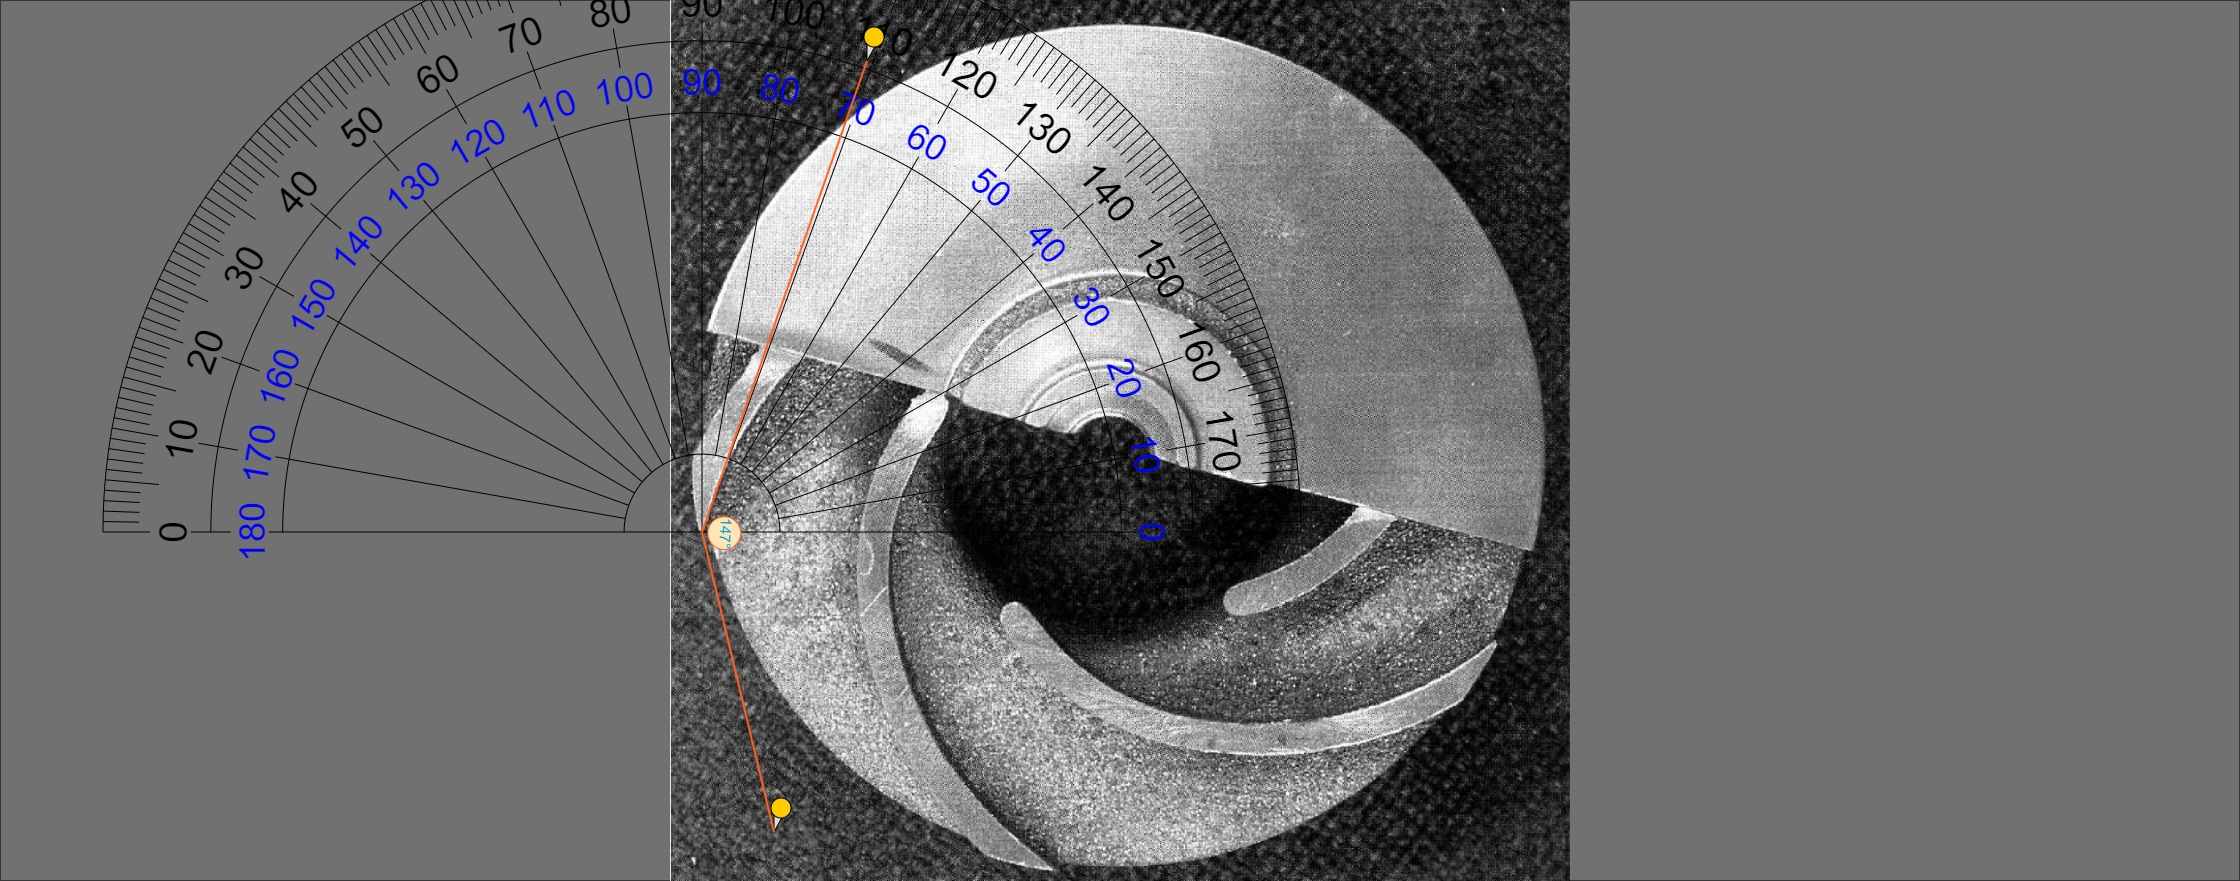
\includegraphics[width=0.7\textwidth]{Sections/Figures/Impeller Angle.jpg}
    \caption{Estimation of the impeller angle using digital protractor}
    \label{fig:impeller_angle}
\end{figure}
The impeller angle was estimated using a digital protractor, as shown in Figure \ref{fig:impeller_angle}. The impeller angle was measured to be 
\begin{align*}
    \beta_2 &= 180^\circ - 147^\circ = 33^\circ
\end{align*}
From equation (\ref{ideal_turbo_machinary}), the ideal operating curve is
\begin{align*}
    \Psi &= 1 - \Phi \cot{\beta_2} \\
    &= 1 - \Phi \cot{33^\circ} \\
    &= 1 - 1.540 \Phi
\end{align*}
\newpage
\section{Appendix: Shut Off Head}
\label{sec:shut_off_head}
Shut off head was discussed in the theory section. From Eq. \ref{eq:shutoff_head} and \ref{eq:thumb_head}, the ideal and "rule of thumb" shut off head can be calculated. The calculation will be performed on the highest experimental speed, $\Omega = \qty{3600}{\rpm}$ which, from Table \ref{tab:single_pump_head_and_flow_coefficients}, the tip speed, $U = \qty{20.4}{\meter\per\second}$. 
\begin{align*}
    H'_\text{ideal} &= \frac{U^2}{g} \\
    &= \frac{(\qty{20.4}{\meter\per\second})^2}{9.81} \\
    &= \qty{42.2}{\meter} \\
    H'_\text{thumb} &= \frac{1}{2} H'_\text{ideal} \\
    &= \frac{1}{2} \times \qty{42.2}{\meter} \\
    &= \qty{21.1}{\meter}
\end{align*}
The actual shutoff head was taken from Table \ref{tab:single_pump_discharge_and_head} and is $\qty{21.8}{\meter}$. The error for the rule of thumb shutoff head can be calculated as
\begin{align*}
    \text{\% Error} &= \bigg|\frac{\text{Experimental} - \text{Theoretical}}{\text{Theoretical}}\bigg| \times 100\% \\
    &= \bigg|\frac{H'_\text{exp} - H'_\text{thumb}}{H'_\text{thumb}}\bigg| \times 100\% \\
    &= \bigg|\frac{21.8 - 21.1}{21.1}\bigg| \times 100\% \\
    &= 3.3\%
\end{align*}
The error for the ideal shutoff head can be calculated as
\begin{align*}
    \text{\% Error} &= \bigg|\frac{\text{Experimental} - \text{Theoretical}}{\text{Theoretical}}\bigg| \times 100\% \\
    &= \bigg|\frac{H'_\text{exp} - H'_\text{ideal}}{H'_\text{ideal}}\bigg| \times 100\% \\
    &= \bigg|\frac{21.8 - 42.2}{42.2}\bigg| \times 100\% \\
    &= 48.3\%
\end{align*}
\newpage
\section{Manufacturer Geometrically Similar and Dissimilar Pumps}
\label{sec:geometrically_similar_pumps}
\begin{longtable}{p{0.15\textwidth}C{0.10\textwidth}C{0.10\textwidth}C{0.10\textwidth}C{0.10\textwidth}C{0.10\textwidth}C{0.10\textwidth}}
    \caption{Geometrically Similar and Dissimilar Pump Dimensions} \\
    \label{tab:geometrically_similar_pumps} \\[-8ex]
    \toprule
    Geometrically Similar & Impeller Diameter, $D$ & Blade Height, $b$ & Blade Width, $w$ & Volumetric Flow, $Q$ & Pump Speed, $N$ & Head, $H$ \\
    & ($\unit{\meter}$) & ($\unit{\meter}$) & ($\unit{\meter}$) & ($\unit{\meter\cubed\per\second}$) & ($\unit{\rpm}$) & ($\unit{\meter}$) \\
    \midrule
    No & 0.108 & 0.009 & 0.0085 & 0.0080 & 3600 & 10.3 \\
    No & 0.108 & 0.009 & 0.0085 & 0.0067 & 3600 & 16.1 \\
    No & 0.108 & 0.009 & 0.0085 & 0.0054 & 3600 & 19.4 \\
    No & 0.108 & 0.009 & 0.0085 & 0.0040 & 3600 & 21.6 \\
    No & 0.108 & 0.009 & 0.0085 & 0.0027 & 3600 & 22.8 \\
    No & 0.102 & 0.009 & 0.0085 & 0.0076 & 3600 & 7.9 \\
    No & 0.102 & 0.009 & 0.0085 & 0.0063 & 3600 & 13.0 \\
    No & 0.102 & 0.009 & 0.0085 & 0.0050 & 3600 & 16.3 \\
    No & 0.102 & 0.009 & 0.0085 & 0.0038 & 3600 & 18.0 \\
    No & 0.102 & 0.009 & 0.0085 & 0.0025 & 3600 & 19.2 \\
    No & 0.096 & 0.009 & 0.0085 & 0.0071 & 3600 & 6.7 \\
    No & 0.096 & 0.009 & 0.0085 & 0.0059 & 3600 & 11.0 \\
    No & 0.096 & 0.009 & 0.0085 & 0.0047 & 3600 & 13.9 \\
    No & 0.096 & 0.009 & 0.0085 & 0.0035 & 3600 & 15.8 \\
    No & 0.096 & 0.009 & 0.0085 & 0.0024 & 3600 & 16.8 \\
    No & 0.083 & 0.009 & 0.0085 & 0.0059 & 3600 & 2.6 \\
    No & 0.083 & 0.009 & 0.0085 & 0.0049 & 3600 & 6.0 \\
    No & 0.083 & 0.009 & 0.0085 & 0.0039 & 3600 & 8.4 \\
    No & 0.083 & 0.009 & 0.0085 & 0.0029 & 3600 & 9.9 \\
    No & 0.083 & 0.009 & 0.0085 & 0.0020 & 3600 & 10.5 \\
    Yes & 0.108 & 0.009 & 0.0085 & 0.0080 & 3600 & 10.3 \\
    Yes & 0.108 & 0.009 & 0.0085 & 0.0067 & 3600 & 16.1 \\
    Yes & 0.108 & 0.009 & 0.0085 & 0.0054 & 3600 & 19.4 \\
    Yes & 0.108 & 0.009 & 0.0085 & 0.0040 & 3600 & 21.6 \\
    Yes & 0.108 & 0.009 & 0.0085 & 0.0027 & 3600 & 22.8 \\
    Yes & 0.102 & 0.009 & 0.00803 & 0.0076 & 3600 & 7.9 \\
    Yes & 0.102 & 0.009 & 0.00803 & 0.0063 & 3600 & 13.0 \\
    Yes & 0.102 & 0.009 & 0.00803 & 0.0050 & 3600 & 16.3 \\
    Yes & 0.102 & 0.009 & 0.00803 & 0.0038 & 3600 & 18.0 \\
    Yes & 0.102 & 0.009 & 0.00803 & 0.0025 & 3600 & 19.2 \\
    Yes & 0.096 & 0.008 & 0.00756 & 0.0071 & 3600 & 6.7 \\
    Yes & 0.096 & 0.008 & 0.00756 & 0.0059 & 3600 & 11.0 \\
    Yes & 0.096 & 0.008 & 0.00756 & 0.0047 & 3600 & 13.9 \\
    Yes & 0.096 & 0.008 & 0.00756 & 0.0035 & 3600 & 15.8 \\
    Yes & 0.096 & 0.008 & 0.00756 & 0.0024 & 3600 & 16.8 \\
    Yes & 0.083 & 0.007 & 0.00653 & 0.0059 & 3600 & 2.6 \\
    Yes & 0.083 & 0.007 & 0.00653 & 0.0049 & 3600 & 6.0 \\
    Yes & 0.083 & 0.007 & 0.00653 & 0.0039 & 3600 & 8.4 \\
    Yes & 0.083 & 0.007 & 0.00653 & 0.0029 & 3600 & 9.9 \\
    Yes & 0.083 & 0.007 & 0.00653 & 0.0020 & 3600 & 10.5 \\
    \bottomrule
\end{longtable}

\begin{longtable}{p{0.15\textwidth}C{0.10\textwidth}C{0.10\textwidth}C{0.10\textwidth}C{0.10\textwidth}C{0.10\textwidth}}
    \caption{Geometrically Similar and Dissimilar Pump Coefficients} \\
    \label{tab:geometrically_similar_pump_coefficients} \\[-8ex]
    \toprule
    Geometrically Similar & Impeller Diameter, $D$ & Impeller Speed, $U$ & Radial Exit Velocity, $v_{2r}$ & Head Coefficient, $\Psi$ & Flow Coefficient, $\Phi$ \\
    & ($\unit{\meter}$) & ($\unit{\meter\per\second}$) & ($\unit{\meter\per\second}$) & & \\
    \midrule
    No & 0.108 & 20.4 & 3.0 & 0.24 & 0.15 \\
    No & 0.108 & 20.4 & 2.5 & 0.38 & 0.12 \\
    No & 0.108 & 20.4 & 2.0 & 0.46 & 0.10 \\
    No & 0.108 & 20.4 & 1.5 & 0.51 & 0.07 \\
    No & 0.108 & 20.4 & 1.0 & 0.54 & 0.05 \\
    No & 0.102 & 19.2 & 3.0 & 0.21 & 0.16 \\
    No & 0.102 & 19.2 & 2.5 & 0.34 & 0.13 \\
    No & 0.102 & 19.2 & 2.0 & 0.43 & 0.10 \\
    No & 0.102 & 19.2 & 1.5 & 0.48 & 0.08 \\
    No & 0.102 & 19.2 & 1.0 & 0.51 & 0.05 \\
    No & 0.096 & 18.1 & 3.0 & 0.20 & 0.17 \\
    No & 0.096 & 18.1 & 2.5 & 0.33 & 0.14 \\
    No & 0.096 & 18.1 & 2.0 & 0.42 & 0.11 \\
    No & 0.096 & 18.1 & 1.5 & 0.47 & 0.08 \\
    No & 0.096 & 18.1 & 1.0 & 0.50 & 0.06 \\
    No & 0.083 & 15.6 & 3.0 & 0.10 & 0.19 \\
    No & 0.083 & 15.6 & 2.5 & 0.24 & 0.16 \\
    No & 0.083 & 15.6 & 2.0 & 0.34 & 0.13 \\
    No & 0.083 & 15.6 & 1.5 & 0.40 & 0.09 \\
    No & 0.083 & 15.6 & 1.0 & 0.42 & 0.07 \\
    Yes & 0.108 & 20.4 & 3.0 & 0.24 & 0.15 \\
    Yes & 0.108 & 20.4 & 2.5 & 0.38 & 0.12 \\
    Yes & 0.108 & 20.4 & 2.0 & 0.46 & 0.10 \\
    Yes & 0.108 & 20.4 & 1.5 & 0.51 & 0.07 \\
    Yes & 0.108 & 20.4 & 1.0 & 0.54 & 0.05 \\
    Yes & 0.102 & 19.2 & 3.2 & 0.21 & 0.17 \\
    Yes & 0.102 & 19.2 & 2.6 & 0.34 & 0.14 \\
    Yes & 0.102 & 19.2 & 2.1 & 0.43 & 0.11 \\
    Yes & 0.102 & 19.2 & 1.6 & 0.48 & 0.08 \\
    Yes & 0.102 & 19.2 & 1.0 & 0.51 & 0.05 \\
    Yes & 0.096 & 18.1 & 3.4 & 0.20 & 0.19 \\
    Yes & 0.096 & 18.1 & 2.8 & 0.33 & 0.15 \\
    Yes & 0.096 & 18.1 & 2.2 & 0.42 & 0.12 \\
    Yes & 0.096 & 18.1 & 1.7 & 0.47 & 0.09 \\
    Yes & 0.096 & 18.1 & 1.1 & 0.50 & 0.06 \\
    Yes & 0.083 & 15.6 & 3.7 & 0.10 & 0.24 \\
    Yes & 0.083 & 15.6 & 3.1 & 0.24 & 0.20 \\
    Yes & 0.083 & 15.6 & 2.5 & 0.34 & 0.16 \\
    Yes & 0.083 & 15.6 & 1.8 & 0.40 & 0.12 \\
    Yes & 0.083 & 15.6 & 1.3 & 0.42 & 0.08 \\
    \bottomrule
\end{longtable}
\subsection{Geometrically Similar Pumps Sample Calculations}
Sample calculations for Table \ref{tab:geometrically_similar_pumps} and Table \ref{tab:geometrically_similar_pump_coefficients} will be shown for an impeller of $D = \qty{102}{\milli\meter}$ and $Q = \qty{0.0076}{\meter\cubed\per\second}$. Pump speed is given as $\qty{3600}{\rpm}$ with number of blades, $N = 5$. Impeller speed is then
\begin{align*}
    U &= \frac{D}{2} \times \Omega \\
    &= \frac{\qty{102}{\milli\meter}}{2} \times \qty{3600}{\rpm} \times \frac{2\pi}{60} \frac{\unit{\radian\per\second}}{\unit{\rpm}} \\
    &= \qty{19.2}{\meter\per\second}
\end{align*}
Geometrically similar means that blade height and width are scaled proportionally to the impeller diameter. Blade height and width are then
\begin{align*}
    b_{102} &= \frac{b_{108} \times D_{102}}{D_{108}} \\
    &= \frac{\qty{9}{\milli\meter} \times \qty{102}{\milli\meter}}{\qty{108}{\milli\meter}} \\
    &= \qty{8.5}{\milli\meter} \\
    w_{102} &= \frac{w_{108} \times D_{102}}{D_{108}} \\
    &= \frac{\qty{8.5}{\milli\meter} \times \qty{102}{\milli\meter}}{\qty{108}{\milli\meter}} \\
    &= \qty{8.03}{\milli\meter}
\end{align*}
Radial exit velocity is then
\begin{align*}
    v_{2r} &= \frac{Q}{b(2\pi r_2 - Nw)} \\
    &= \frac{\qty{0.0076}{\meter\cubed\per\second}}{\qty{8.5}{\milli\meter} \times (\pi \times \qty{0.102}{\meter} - 5 \times \qty{8.03}{\milli\meter})} \\
    &= \qty{3.0}{\meter\per\second}
\end{align*}
Head coefficient is then
\begin{align*}
    \Psi &= \frac{H}{U^2} \\
    &= \frac{\qty{7.9}{\meter}}{\qty{19.2}{\meter\per\second}} \\
    &= 0.41
\end{align*}
Flow coefficient is then
\begin{align*}
    \Phi &= \frac{Q}{U \times D^2} \\
    &= \frac{\qty{0.0076}{\meter\cubed\per\second}}{\qty{19.2}{\meter\per\second} \times (\qty{0.102}{\meter})^2} \\
    &= 0.16
\end{align*}

\subsection{Geometrically Dissimilar Pumps Sample Calculations}
Sample calculations for Table \ref{tab:geometrically_similar_pumps} and Table \ref{tab:geometrically_similar_pump_coefficients} will be shown for an impeller of $D = \qty{102}{\milli\meter}$ and $Q = \qty{0.0076}{\meter\cubed\per\second}$. Pump speed is given as $\qty{3600}{\rpm}$ with number of blades, $N = 5$. Impeller speed is then
\begin{align*}
    U &= \frac{D}{2} \times \Omega \\
    &= \frac{\qty{102}{\milli\meter}}{2} \times \qty{3600}{\rpm} \times \frac{2\pi}{60} \frac{\unit{\radian\per\second}}{\unit{\rpm}} \\
    &= \qty{19.2}{\meter\per\second}
\end{align*}
Geometrically dissimilar means that blade height and width are not scaled proportionally to the impeller diameter. Blade height and width are unchanged between all pumps. That is,
\begin{align*}
    b_{102} &= b_{108}  \\
    &= \qty{9}{\milli\meter} \\
    w_{102} &= w_{108}  \\
    &= \qty{8.5}{\milli\meter}
\end{align*}
Radial exit velocity is then
\begin{align*}
    v_{2r} &= \frac{Q}{b(2\pi r_2 - Nw)} \\
    &= \frac{\qty{0.0076}{\meter\cubed\per\second}}{\qty{9}{\milli\meter} \times (\pi \times \qty{0.102}{\meter} - 5 \times \qty{8.5}{\milli\meter})} \\
    &= \qty{3.2}{\meter\per\second}
\end{align*}
Head coefficient is then
\begin{align*}
    \Psi &= \frac{H}{U^2} \\
    &= \frac{\qty{7.9}{\meter}}{\qty{19.2}{\meter\per\second}} \\
    &= 0.41
\end{align*}
Flow coefficient is then
\begin{align*}
    \Phi &= \frac{Q}{U \times D^2} \\
    &= \frac{\qty{0.0076}{\meter\cubed\per\second}}{\qty{19.2}{\meter\per\second} \times (\qty{0.102}{\meter})^2} \\
    &= 0.16
\end{align*}

% \section{Figures}
\label{sec:figures}
\begin{figure}[h]
    \centering
    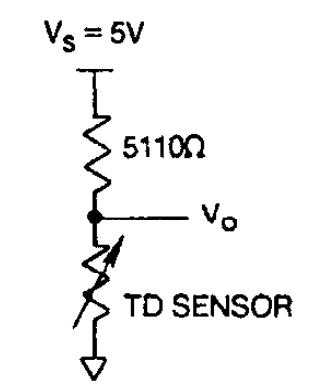
\includegraphics[width=0.25\textwidth]{Appendix/TD5A_circuit.png}
    \caption{Schematic of the circuit for the Honeywell TD5A temperature sensor}
    \label{fig:TD5A_circuit}
\end{figure}

\begin{figure}[h]
    \centering
    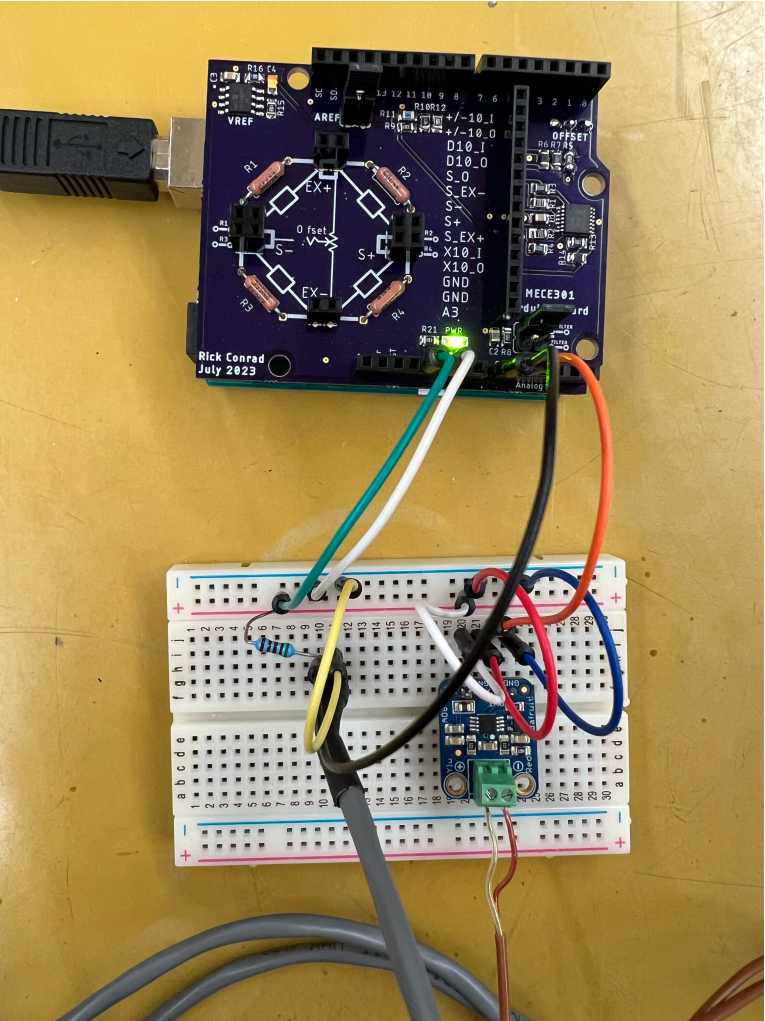
\includegraphics[width=0.4\textwidth]{Appendix/lab_manual_circuit.png}
    \caption{Built circuit for the Honeywell TD5A temperature sensor}
    \label{fig:lab_manual_circuit}
\end{figure}

% linear regression for thermistor and thermocouple
\begin{figure}[h]
    \centering
    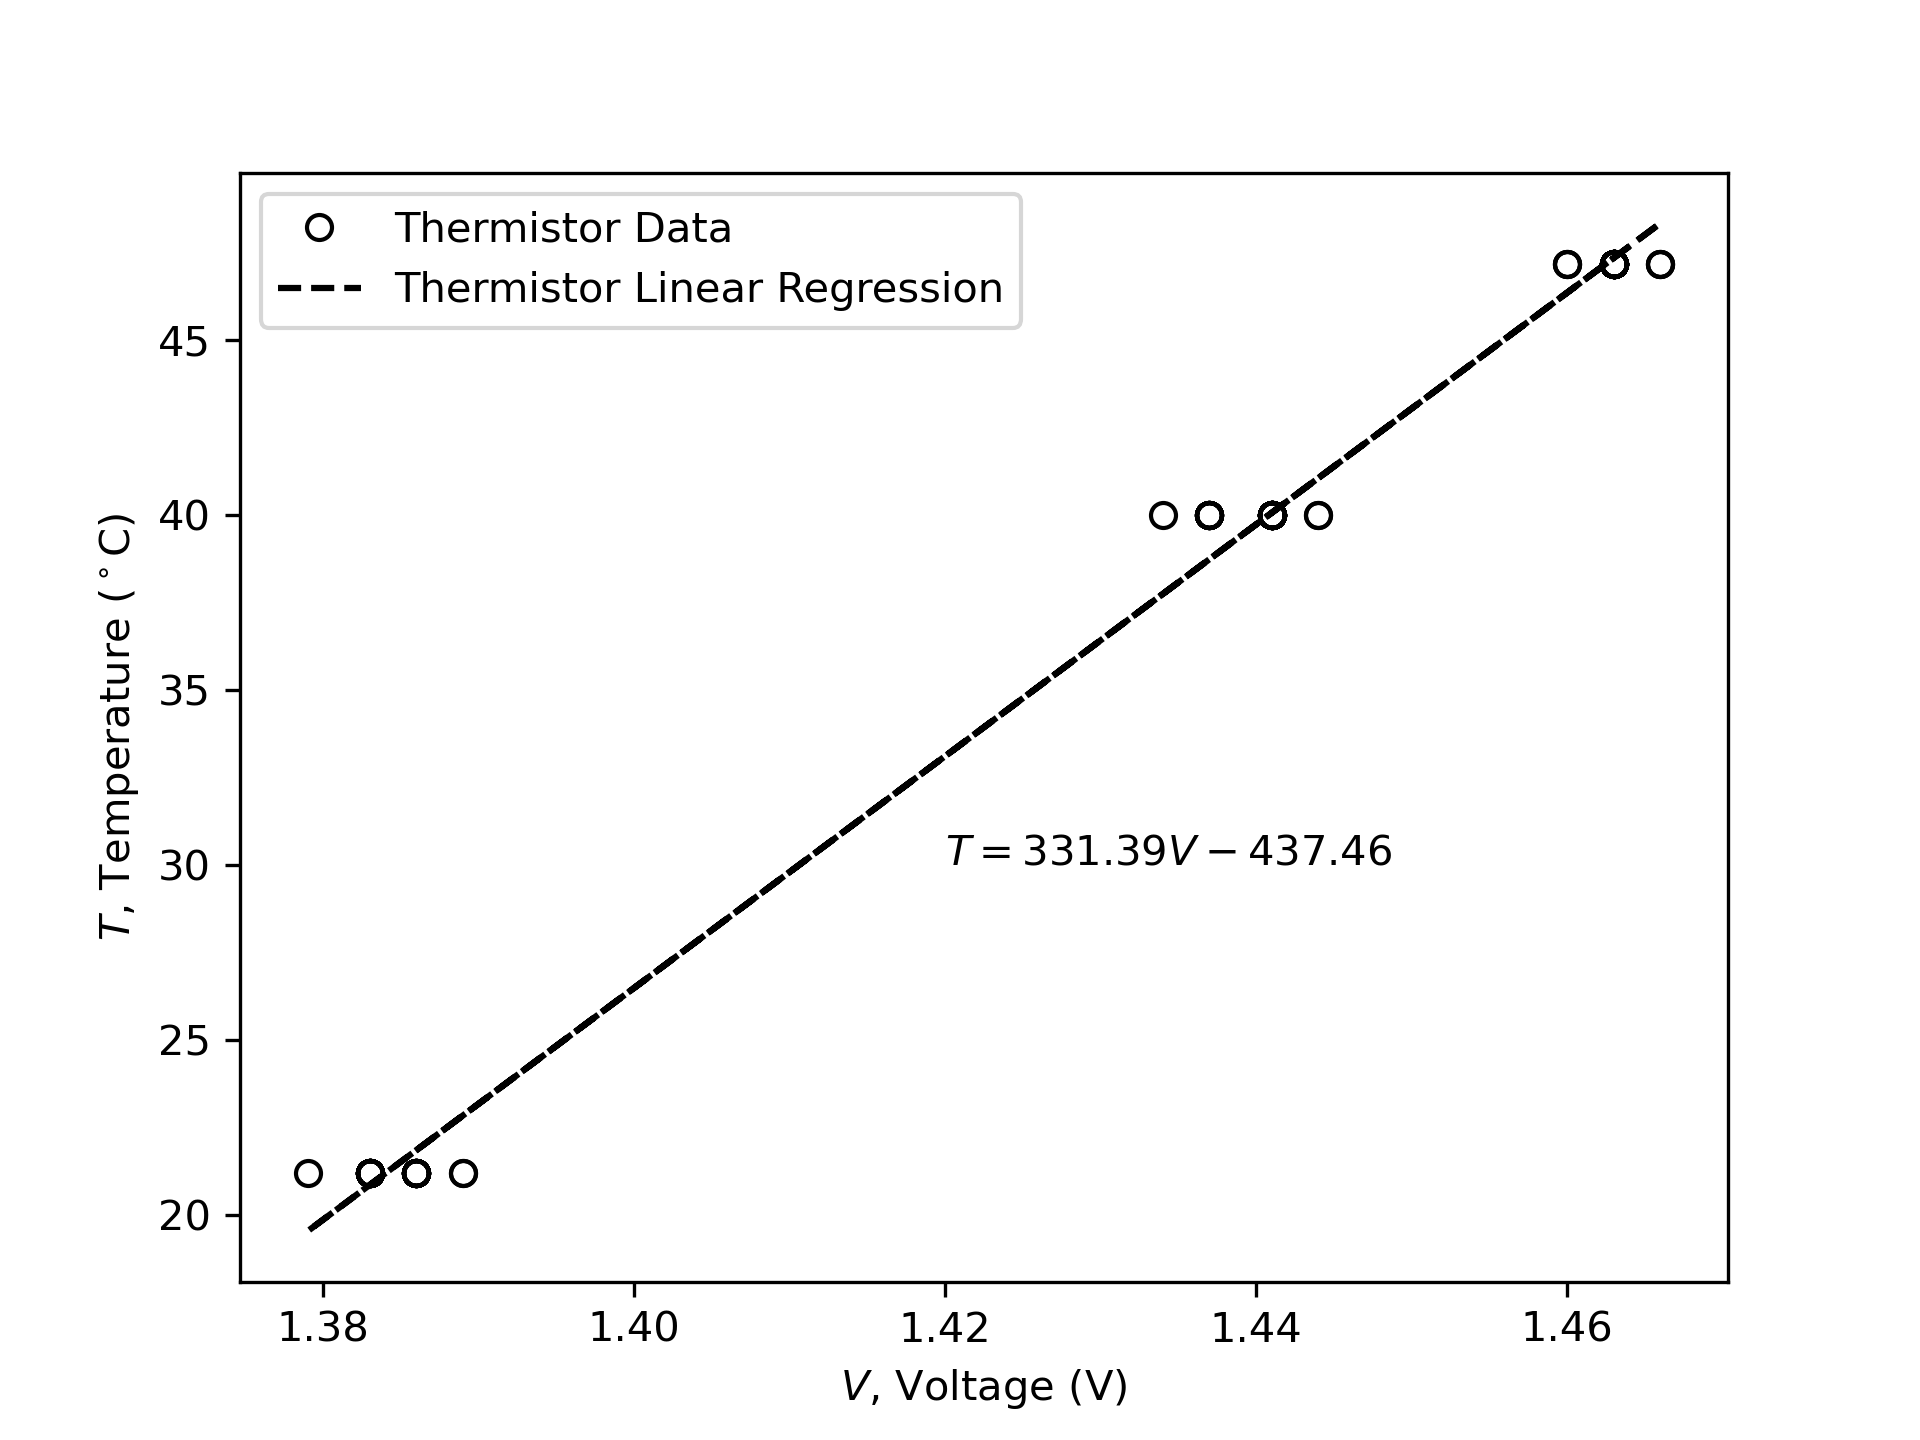
\includegraphics[width=0.5\textwidth]{matplotlib/thermistor.png}
    \caption{Linear fit for the thermistor}
    \label{fig:thermistor_calibration}
\end{figure}

\begin{figure}[h]
    \centering
    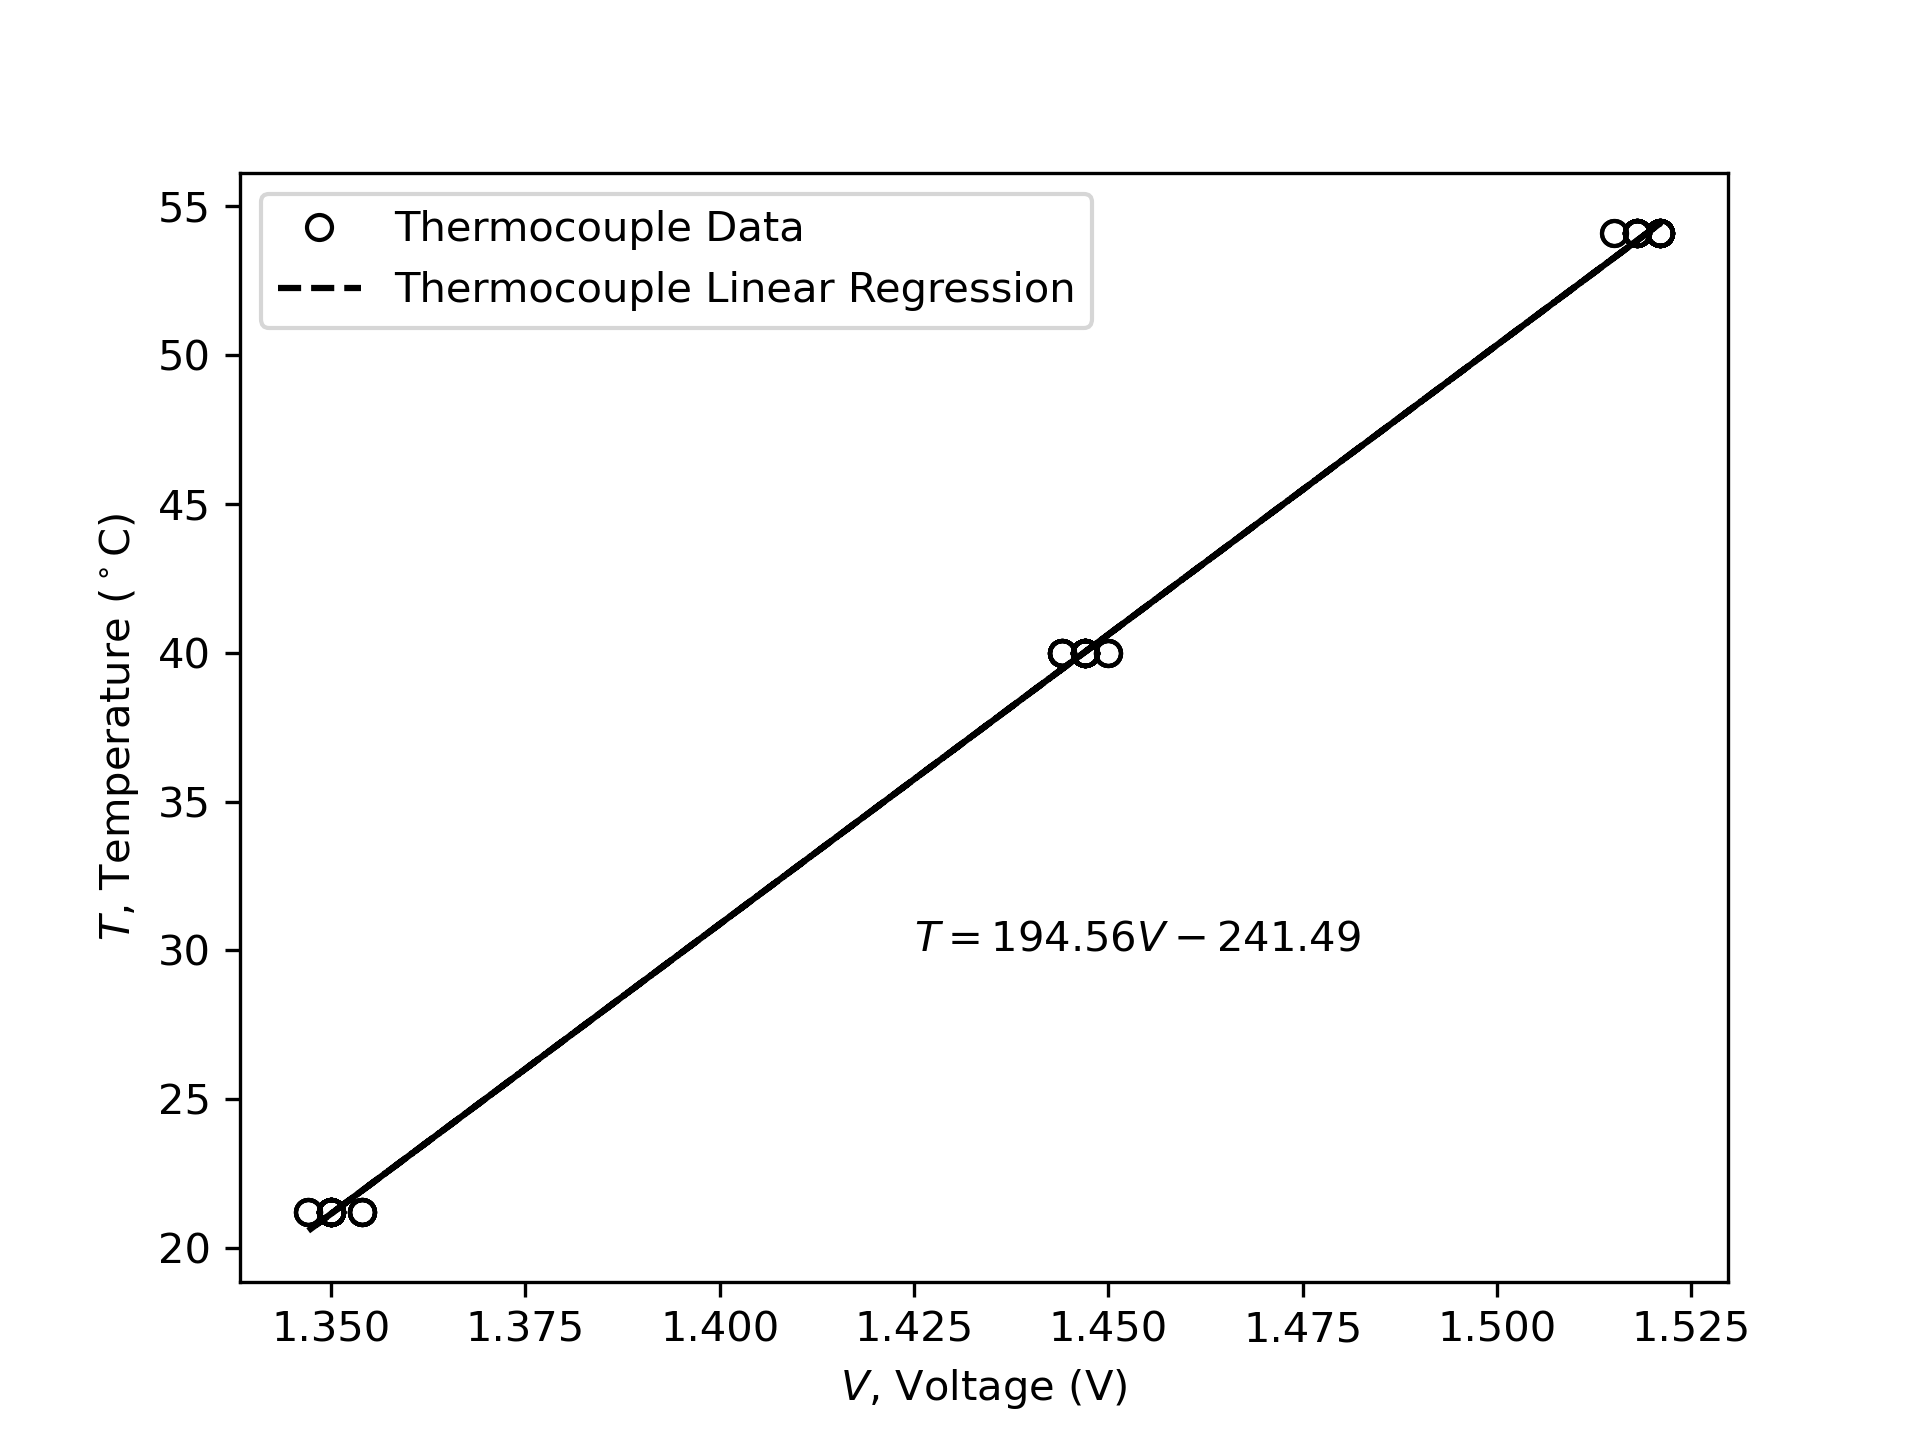
\includegraphics[width=0.5\textwidth]{matplotlib/thermocouple.png}
    \caption{Linear fit for the thermocouple}
    \label{fig:thermocouple_calibration}
\end{figure}

\begin{figure}[h]
    \centering
    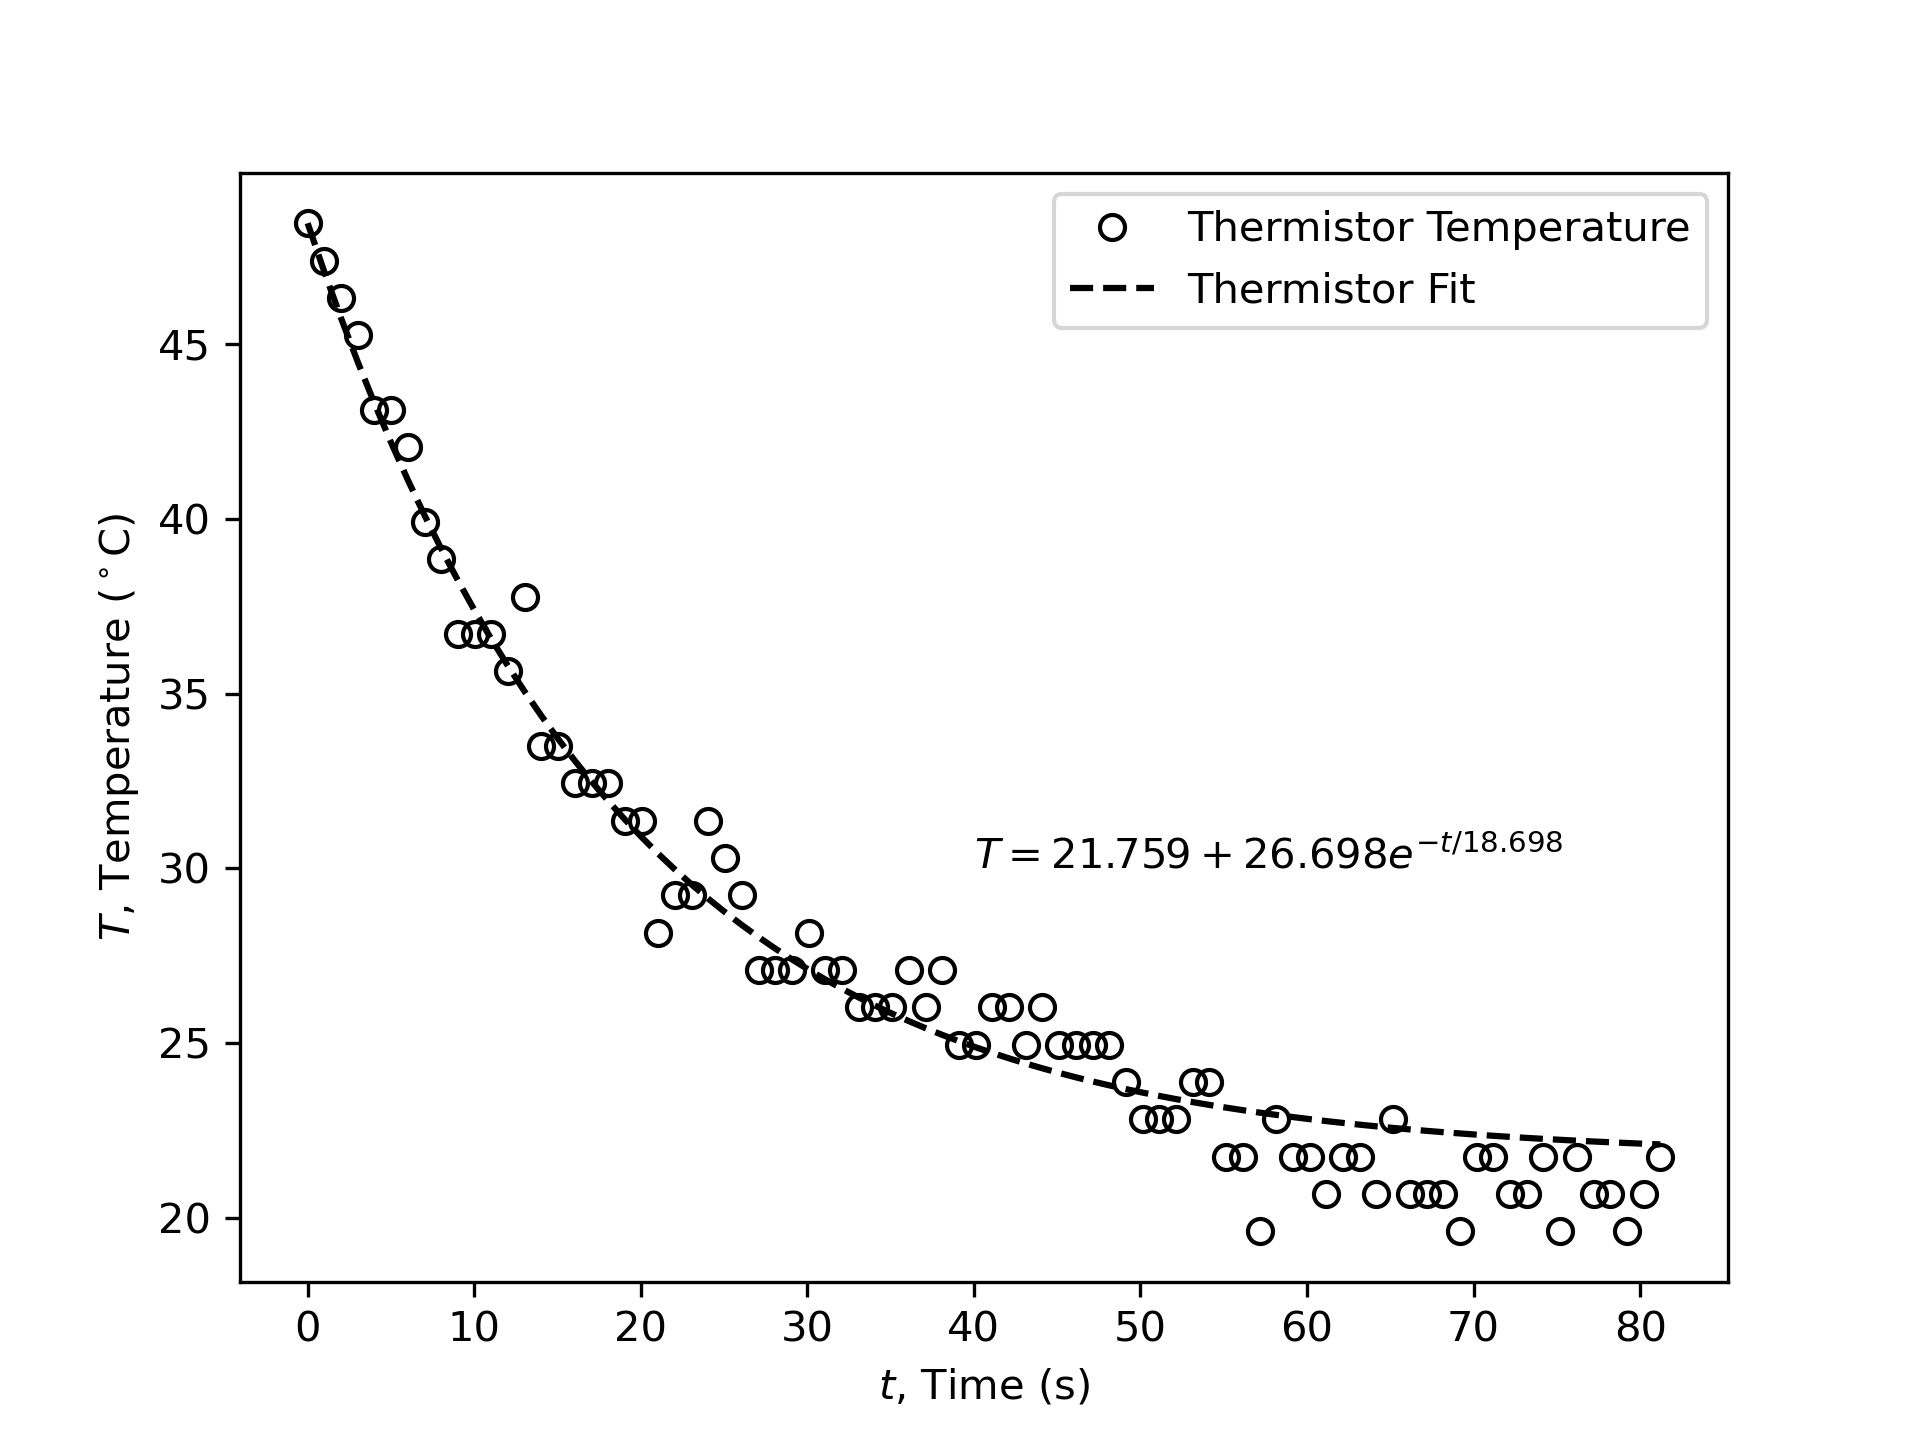
\includegraphics[width=0.5\textwidth]{matplotlib/thermistor_transient_air.png}
    \caption{Transient response of the thermistor in air}
    \label{fig:thermistor_transient_air}
\end{figure}

\begin{figure}[h]
    \centering
    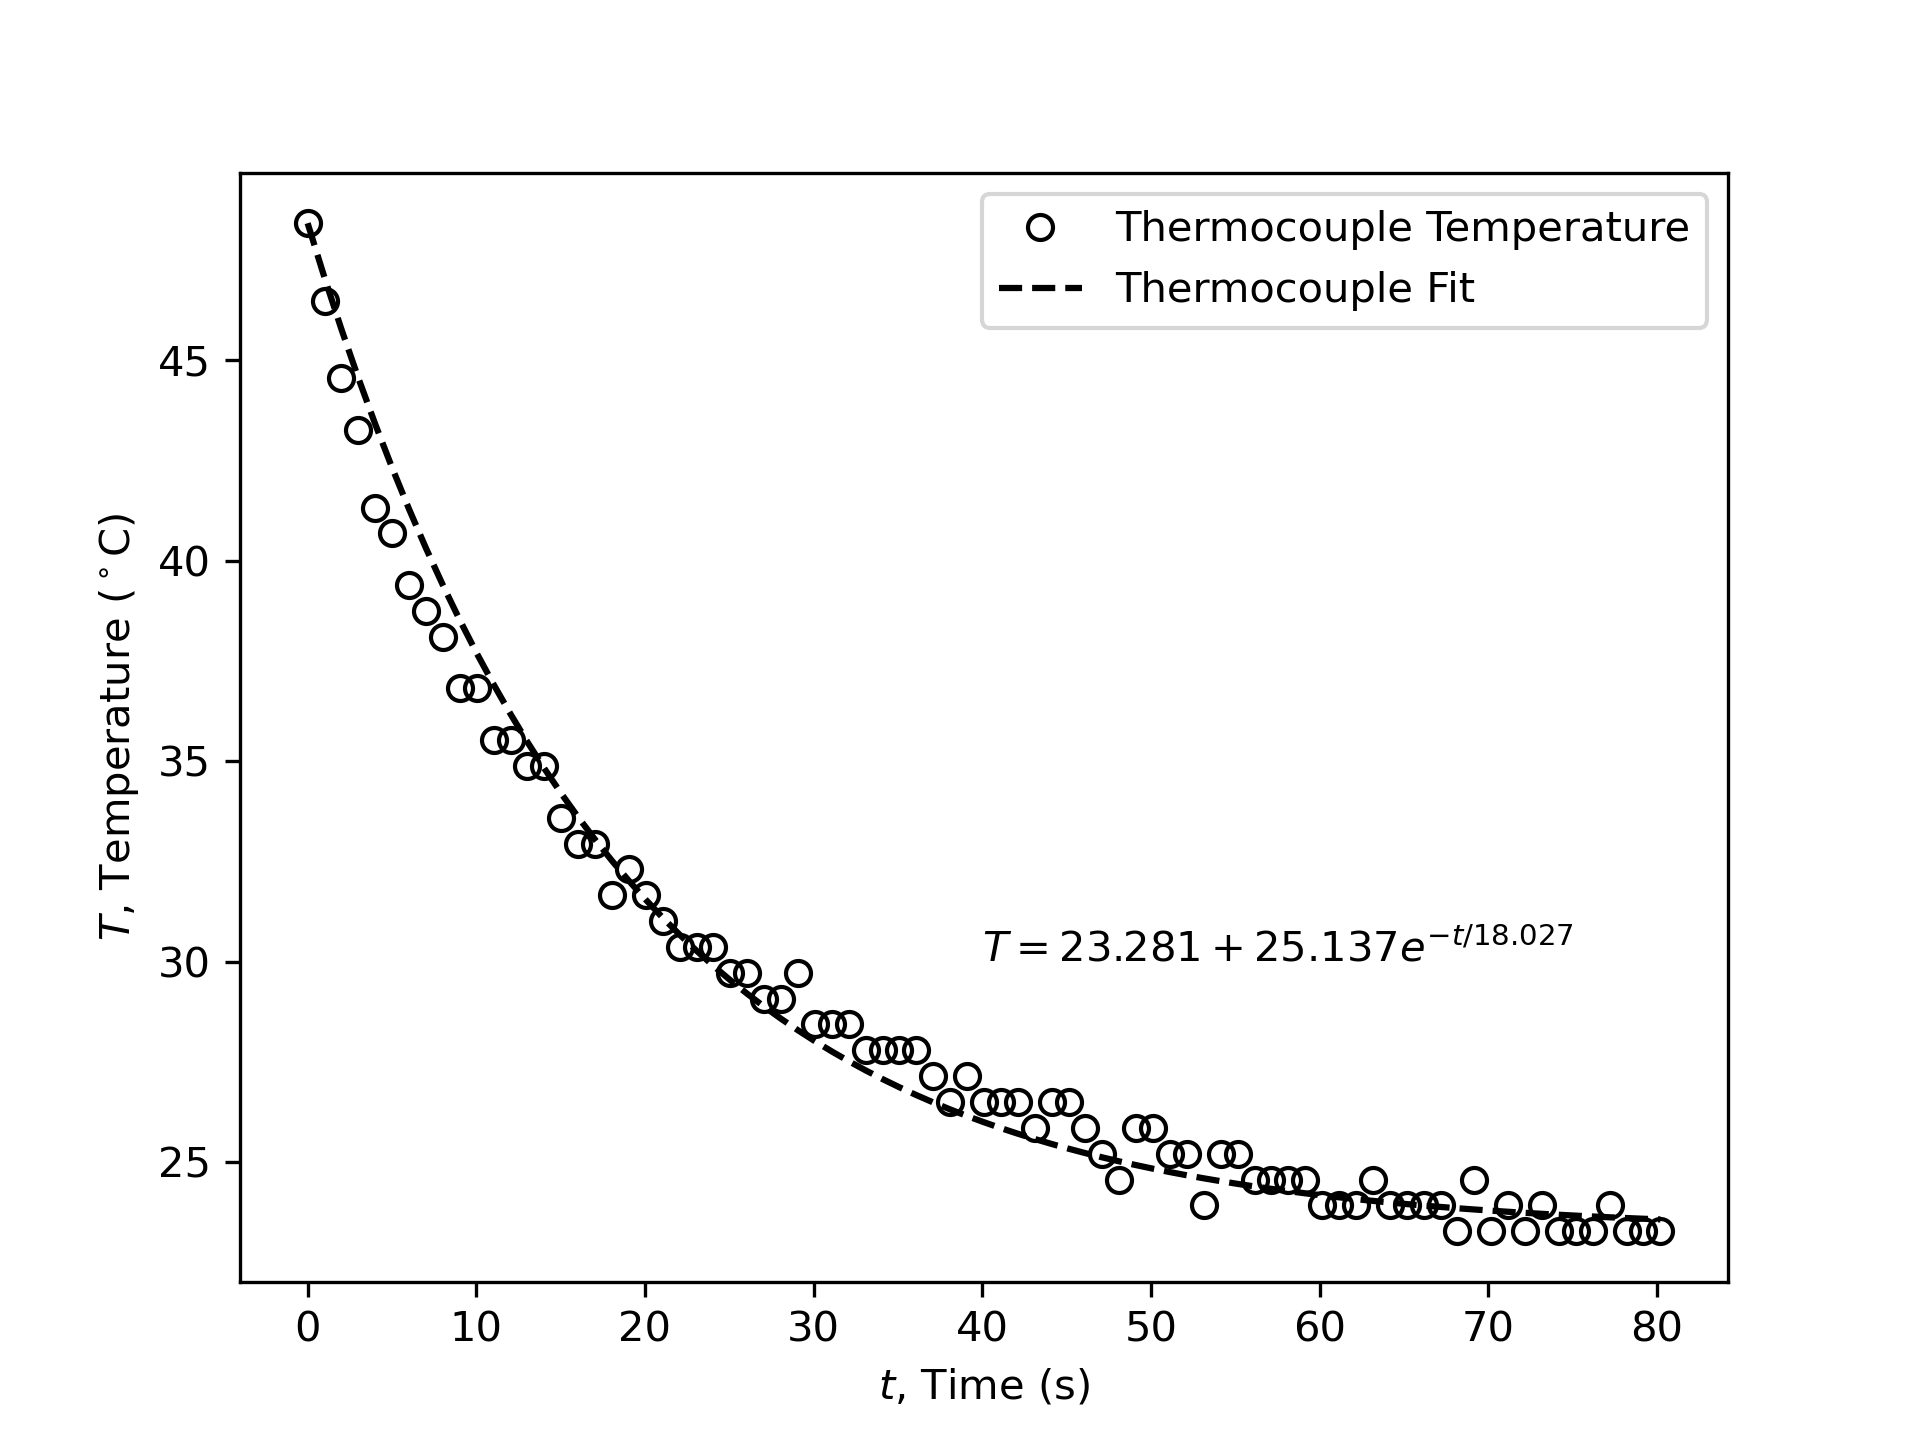
\includegraphics[width=0.5\textwidth]{matplotlib/thermocouple_transient_air.png}
    \caption{Transient response of the thermocouple in air}
    \label{fig:thermocouple_transient_air}
\end{figure}

\begin{figure}[h]
    \centering
    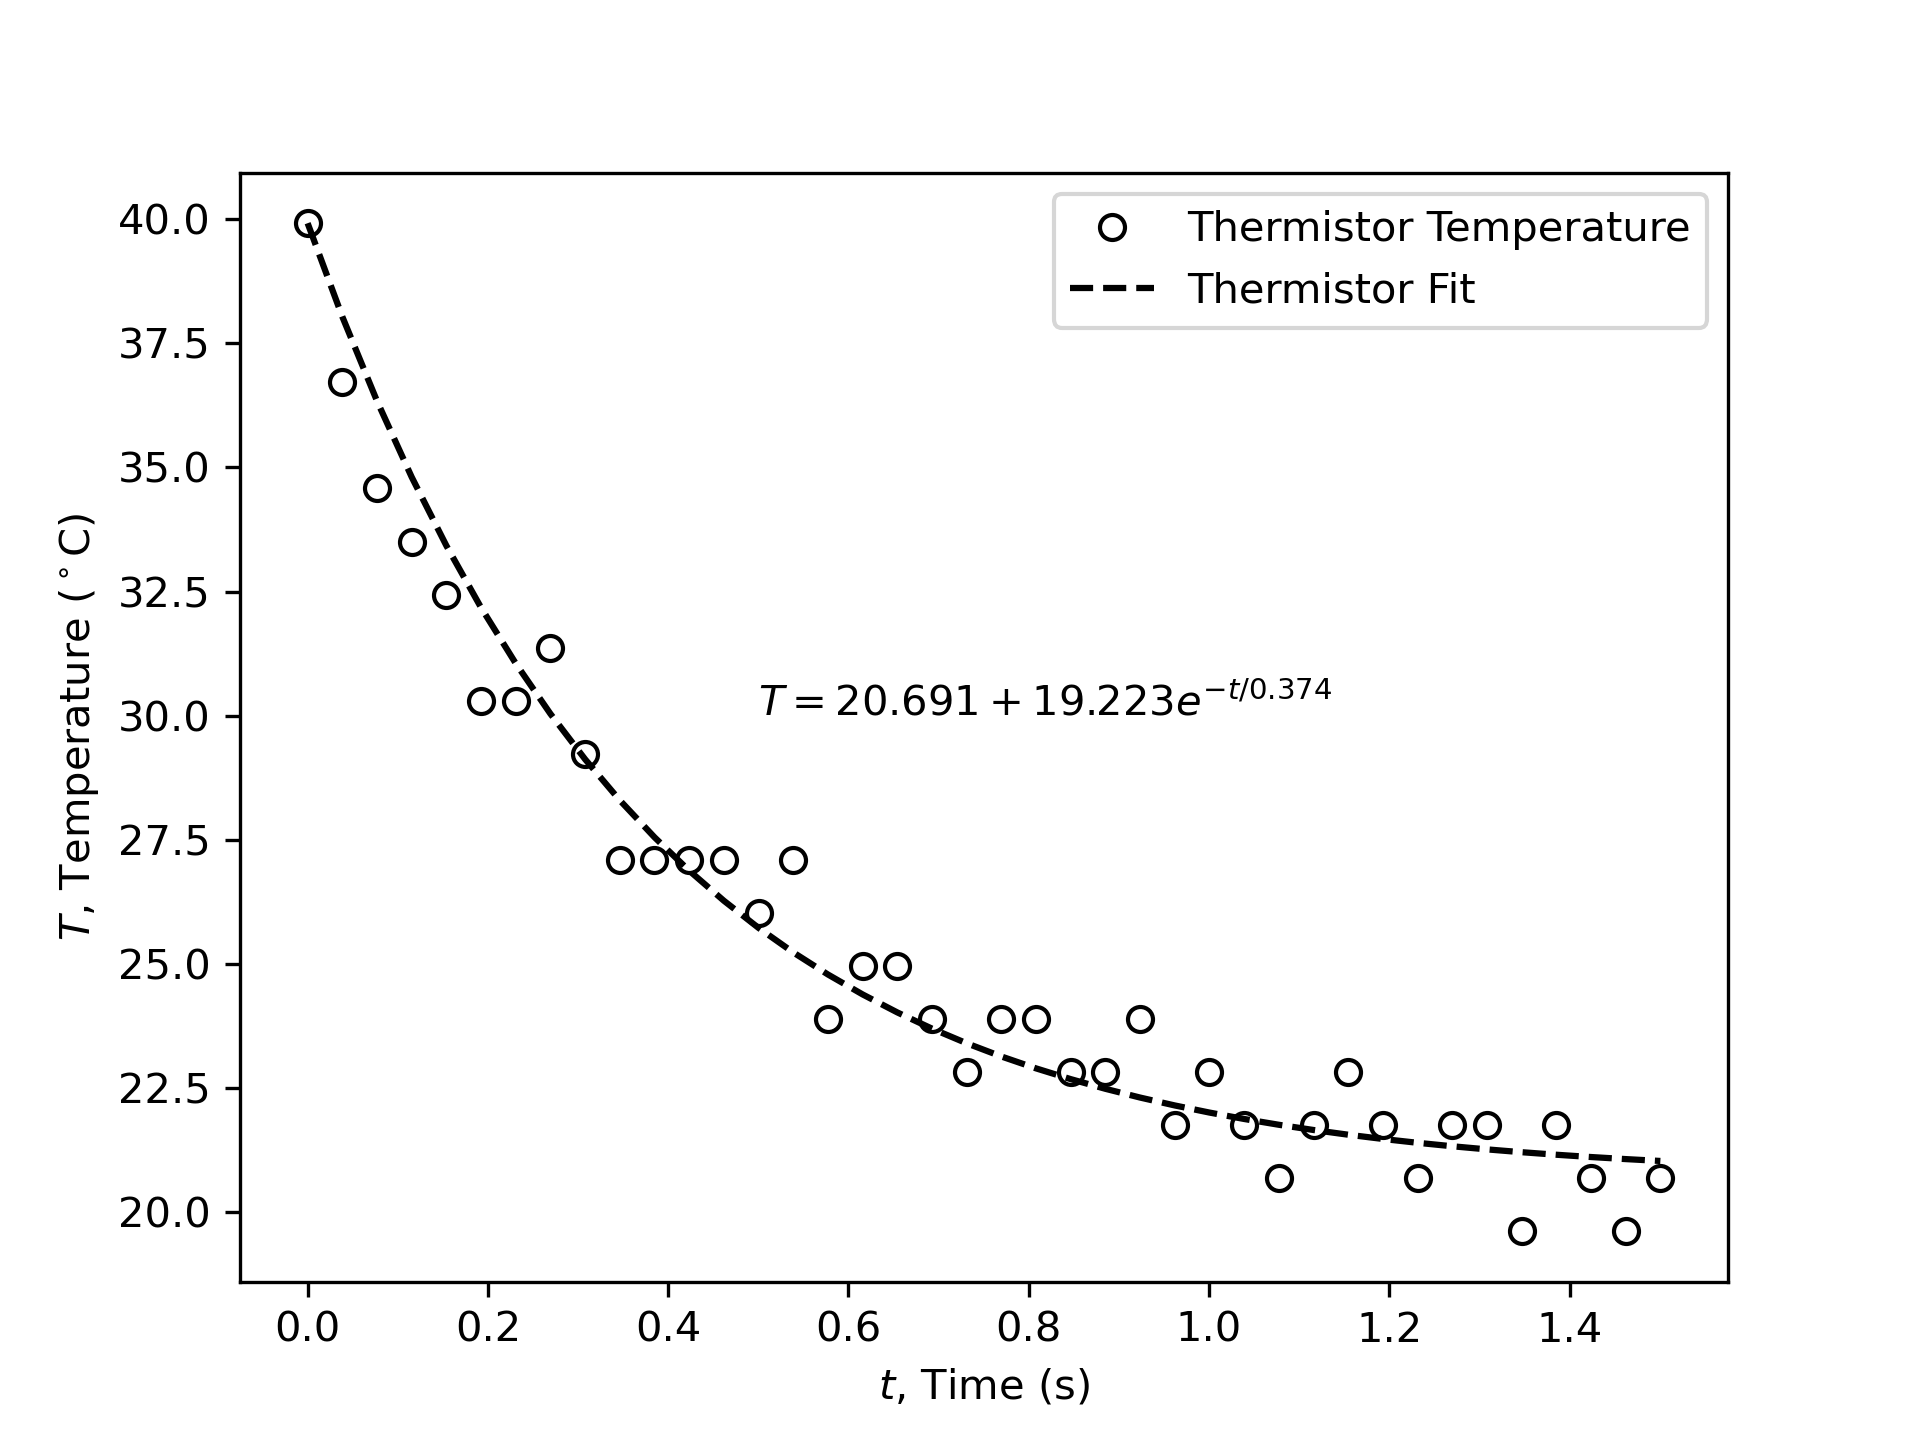
\includegraphics[width=0.5\textwidth]{matplotlib/thermistor_transient_water.png}
    \caption{Transient response of the thermistor in water}
    \label{fig:thermistor_transient_water}
\end{figure}

\begin{figure}[h]
    \centering
    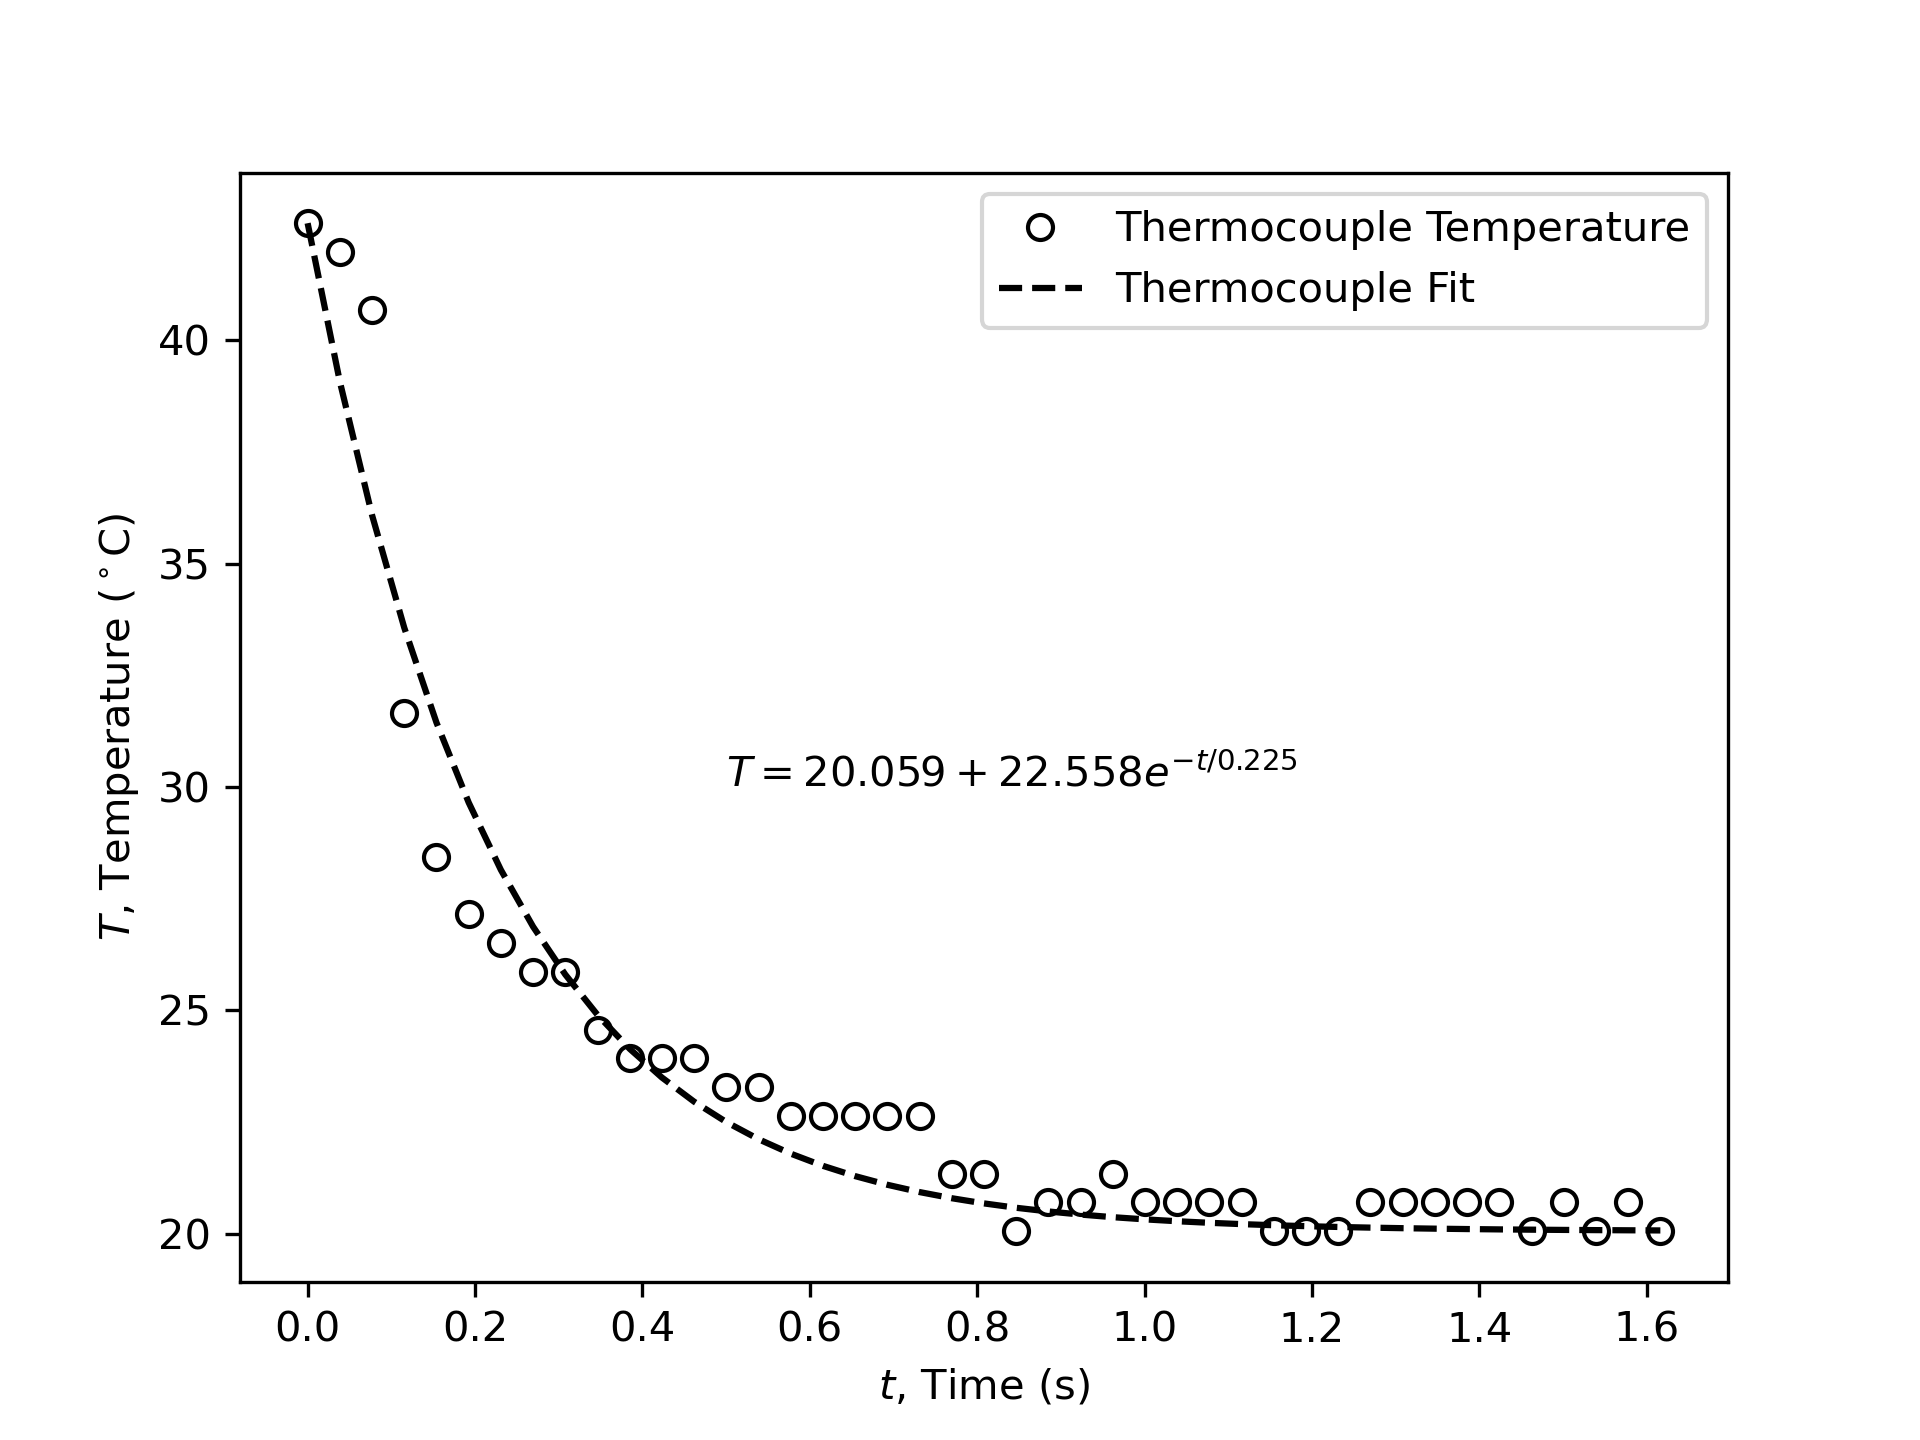
\includegraphics[width=0.5\textwidth]{matplotlib/thermocouple_transient_water.png}
    \caption{Transient response of the thermocouple in water}
    \label{fig:thermocouple_transient_water}
\end{figure}

\FloatBarrier

% invisible character
% \newpage
% \section{Tables}
\label{sec:tables}

% head of deviation table for thermistor
% use 1 decimal place for temperature
% Thermistor Deviation Table						
% 21.2	0.643941754	0.643941754	0.643941754	0.643941754	0.643941754	0.643941754
% 40	-1.255340005	-1.255340005	-2.249499902	0.070206523	0.070206523	0.070206523
% 46.9	0.460712431	0.460712431	0.460712431	-0.533447465	0.460712431	0.460712431
\begin{table}[h]
    \centering
    \caption{Deviation table for the thermistor}
    \label{tab:thermistor_calibration_deviation}
    \begin{tabular}{ccccccccc}
        \toprule
        Reference Temperature & \multicolumn{6}{c}{Measured Temperature} &  & Max Deviation \\
        \cmidrule{2-7}
        ($^\circ$C) & ($^\circ$C) & ($^\circ$C) & ($^\circ$C) & ($^\circ$C) & ($^\circ$C) & ($^\circ$C) &  & ($^\circ$C) \\
        \midrule
        21.2 & 0.6 & 0.6 & 0.6 & 0.6 & 0.6 & 0.6 & ... & 3.3 \\
        40.0 & -1.3 & -1.3 & -2.2 & 0.1 & 0.1 & 0.1 & ... & 3.3 \\
        46.9 & 0.5 & 0.5 & 0.5 & -0.5 & 0.5 & 0.5 & ... & 2.0 \\
        \bottomrule
    \end{tabular}
\end{table}

% head of deviation table for thermocouple 
% Thermocouple Deviation Table						
% 21.2	-1.141	-1.141	-1.141	-1.141	-1.141	-1.141
% 40	-0.605	-0.605	-0.605	-0.605	-0.605	-1.25
% 53.5	0.719	0.719	0.074	0.719	0.719	0.074
% Max Deviation
% 21.2	1.289
% 40	1.289
% 53.5	1.289
\begin{table}[h]
    \centering
    \caption{Head of deviation table for the thermocouple using Adafruit conversion equation}
    \label{tab:thermocouple_calibration_deviation_adafruit}
    \begin{tabular}{ccccccccc}
        \toprule
        Reference Temperature & \multicolumn{6}{c}{Measured Temperature} &  & Max Deviation \\
        \cmidrule{2-7}
        ($^\circ$C) & ($^\circ$C) & ($^\circ$C) & ($^\circ$C) & ($^\circ$C) & ($^\circ$C) & ($^\circ$C) &  & ($^\circ$C) \\
        \midrule
        21.2 & -1.1 & -1.1 & -1.1 & -1.1 & -1.1 & -1.1 &  ... & 1.3 \\
        40.0 & -0.6 & -0.6 & -0.6 & -0.6 & -0.6 & -1.3 &  ... & 1.3 \\
        53.5 & 0.7 & 0.7 & 0.1 & 0.7 & 0.7 & 0.1 &  ... & 1.3 \\
        \bottomrule
    \end{tabular}
\end{table}

% head of deviation table for thermocouple with linear fit
% Thermocouple linear fit deviation table						
% 21.2	0.0	0.0	0.0	0.0	0.0	0.0
% 40	0.0	0.0	0.0	0.0	0.0	-0.6
% 54.1	0.3	0.3	-0.3	0.3	0.3	-0.3
% Max Deviation
% 21.2	1.4
% 40	1.2
% 53.5	1.2
\begin{table}[h]
    \centering
    \caption{Head of deviation table for the thermocouple using linear fit}
    \label{tab:thermocouple_calibration_deviation_linear}
    \begin{tabular}{ccccccccc}
        \toprule
        Reference Temperature & \multicolumn{6}{c}{Measured Temperature} &  & Max Deviation \\
        \cmidrule{2-7}
        ($^\circ$C) & ($^\circ$C) & ($^\circ$C) & ($^\circ$C) & ($^\circ$C) & ($^\circ$C) & ($^\circ$C) &  & ($^\circ$C) \\
        \midrule
        21.2 & 0.0 & 0.0 & 0.0 & 0.0 & 0.0 & 0.0 &  ... & 1.4 \\
        40.0 & 0.0 & 0.0 & 0.0 & 0.0 & 0.0 & -0.6 &  ... & 1.2 \\
        53.5 & 0.3 & 0.3 & -0.3 & 0.3 & 0.3 & -0.3 &  ... & 1.2 \\
        \bottomrule
    \end{tabular}
\end{table}

% Transient response in air
% Table 2.0: Cooling in air experiment			
% Time (microseconds)	Thermistor Temperature (C)	Thermistor Response	Thermistor (Exp-Theor)^2
% 0	48.457	48.457	0
% 1.002568	47.389	47.06318374	0.106156236
% 2.005144	46.321	45.74212386	0.33509759
% 3.00772	45.253	44.49003277	0.582118987
% 4.01028	43.117	43.30332826	0.034718222
% 5.01284	43.117	42.17857728	0.880637207
% 6.0154	42.049	41.11254545	0.87694713

\begin{table}
    \centering
    \caption{Transient response of the thermistor in air}
    \label{tab:thermistor_transient_air}
    \begin{tabular}{ccccc}
        \toprule
        Time & Thermistor  & Thermistor Model  & $(\Delta T_{\text{thermistor}})^2$ \\
        (s) & ($^\circ$C) & ($^\circ$C) & ($^circ$C$^2$)\\
        \midrule
        0.000 & 48.457 & 48.457 & 0.000 \\
        1.003 & 47.389 & 47.063 & 0.106 \\
        2.005 & 46.321 & 45.742 & 0.335 \\
        3.008 & 45.253 & 44.490 & 0.582 \\
        4.010 & 43.117 & 43.303 & 0.035 \\
        5.013 & 43.117 & 42.179 & 0.881 \\
        6.015 & 42.049 & 41.113 & 0.877 \\
        \bottomrule
    \end{tabular}
\end{table}

% Table 2.0: Cooling in air experiment			
% Time (microseconds)	Thermocouple Temperature (C)	Thermocouple Response	Thermocouple (Exp-Theor)^2
% 0	48.418	48.418	0
% 1.002568	46.484	47.05814709	0.329644885
% 2.005144	44.551	45.77184907	1.490472446
% 3.00772	43.262	44.5551373	1.672204067
% 4.01028	41.328	43.40426516	4.310877004
% 5.01284	40.684	42.31565203	2.662288336
% 6.0154	39.395	41.28592986	3.575615747
\begin{table}
    \centering
    \caption{Transient response of the thermocouple in air}
    \label{tab:thermocouple_transient_air}
    \begin{tabular}{ccccc}
        \toprule
        Time & Thermocouple  & Thermocouple Model  & $(\Delta T_{\text{thermocouple}})^2$ \\
        (s) & ($^\circ$C) & ($^\circ$C) & ($^\circ$C$^2$)\\
        \midrule
        0.000 & 48.418 & 48.418 & 0.000 \\
        1.003 & 46.484 & 47.058 & 0.330 \\
        2.005 & 44.551 & 45.772 & 1.490 \\
        3.008 & 43.262 & 44.555 & 1.672 \\
        4.010 & 41.328 & 43.404 & 4.311 \\
        5.013 & 40.684 & 42.316 & 2.662 \\
        6.015 & 39.395 & 41.286 & 3.576 \\
        \bottomrule
    \end{tabular}
\end{table}
% Table 2.1: Cooling in water experiment			
% Time (microseconds)	Thermistor Temperature (C)	Thermistor Response	Thermistor (Exp-Theor)^2
% 0	39.914	39.914	0
% 0.03848	36.71	38.03237331	1.748671173
% 0.07696	34.574	36.33492802	3.100867488
% 0.11544	33.506	34.80363569	1.683858378
% 0.15392	32.438	33.42223258	0.968713769
% 0.1924	30.302	32.17604692	3.512051841
\begin{table}
    \centering
    \caption{Transient response of the thermistor in water}
    \label{tab:thermistor_transient_water}
    \begin{tabular}{ccccc}
        \toprule
        Time & Thermistor  & Thermistor Model  & $(\Delta T_{\text{thermistor}})^2$ \\
        (s) & ($^\circ$C) & ($^\circ$C) & ($^\circ$C$^2$)\\
        \midrule
        0.000 & 39.914 & 39.914 & 0.000 \\
        0.038 & 36.710 & 38.032 & 1.749 \\
        0.077 & 34.574 & 36.335 & 3.101 \\
        0.115 & 33.506 & 34.804 & 1.684 \\
        0.154 & 32.438 & 33.422 & 0.969 \\
        0.192 & 30.302 & 32.176 & 3.512 \\
        \bottomrule
    \end{tabular}
\end{table}
% Table 2.1: Cooling in water experiment			
% Time (microseconds)	Thermocouple Temperature (C)	Thermocouple Response	Thermocouple (Exp-Theor)^2
% 0	42.617	42.617	0
% 0.03848	41.973	39.07143777	8.419063359
% 0.07696	40.684	36.08315064	21.16781486
% 0.11544	31.66	33.56454867	3.627305627
% 0.15392	28.437	31.44180892	9.028876648
% 0.1924	27.148	29.6527116	6.2735802
\begin{table}
    \centering
    \caption{Transient response of the thermocouple in water}
    \label{tab:thermocouple_transient_water}
    \begin{tabular}{ccccc}
        \toprule
        Time & Thermocouple  & Thermocouple Model  & $(\Delta T_{\text{thermocouple}})^2$ \\
        (s) & ($^\circ$C) & ($^\circ$C) & ($^\circ$C$^2$)\\
        \midrule
        0.000 & 42.617 & 42.617 & 0.000 \\
        0.038 & 41.973 & 39.071 & 8.419 \\
        0.077 & 40.684 & 36.083 & 21.168 \\
        0.115 & 31.660 & 33.565 & 3.627 \\
        0.154 & 28.437 & 31.442 & 9.029 \\
        0.192 & 27.148 & 29.653 & 6.274 \\
        \bottomrule
    \end{tabular}
\end{table}

% Air		Water	
% Thermistor	Thermocouple	Thermistor	Thermocouple
% T_0	48.457	48.418	39.914	42.617
% T_infty	21.759	23.281	20.691	20.059
% tau	18.69803057	18.02662691	0.373547583	0.225033996
% SS	122.338	46.26568305	35.74509399	69.88833339
\begin{table}
    \centering
    \caption{Steady state temperature and time constant for the thermistor and thermocouple in air and water}
    \label{tab:steady_state_time_constant}
    \begin{tabular}{ccccc}
        \toprule
        & \multicolumn{2}{c}{Air} & \multicolumn{2}{c}{Water} \\
        \cmidrule{2-3} \cmidrule{4-5}
        & Thermistor & Thermocouple & Thermistor & Thermocouple \\  
        \midrule
        $T_0$ & $\qty{48.457}{\celsius}$ & $\qty{48.418}{\celsius}$ & $\qty{39.914}{\celsius}$ & $\qty{42.617}{\celsius}$ \\
        $T_\infty$ & $\qty{21.759}{\celsius}$ & $\qty{23.281}{\celsius}$ & $\qty{20.691}{\celsius}$ & $\qty{20.059}{\celsius}$ \\
        $\tau$ & $\qty{18.698}{\second}$ & $\qty{18.027}{\second}$ & $\qty{0.374}{\second}$ & $\qty{0.225}{\second}$ \\
        SS & $\qty{122.338}{\celsius}$ & $\qty{46.266}{\celsius}$ & $\qty{35.745}{\celsius}$ & $\qty{69.888}{\celsius}$ \\
        \bottomrule
    \end{tabular}
\end{table}


% \newpage
% \section{Appendix: Thermistor and Thermocouple Calibration}

\noindent For the thermistor, a linear fit was obtained using Excel's \texttt{LINEST} function. The fit is shown in Figure \ref{fig:thermistor_calibration}
The fit equation is 
\begin{equation}
    T = 331.39 V  -437.46 \label{eq:thermistor_calibration}
\end{equation}

A deviation table was generated using the fit equation to map the thermistor voltage to temperature. The head of the table is shown in 
Table \ref{tab:thermistor_calibration_deviation}. The full table is available in the Excel file submitted with this report.

Deviation was determined by 
\begin{equation}
    \Delta T  = T_{\text{meas}} - T_{\text{ref}} \nonumber
\end{equation}
For the thermistor first measurement at 21.2$^\circ$C, the deviation was
\begin{equation}
    \Delta T = 21.8 - 21.2 = \qty{0.6}{\celsius} \nonumber
\end{equation}

The accuracy of the thermistor was determined by taking the maximum absolute deviation from the reference temperature across all measurements. The 
accuracy was determined to be
\begin{equation}
    Accuracy = \text{max}(|\{\Delta T_{i, j}, \forall i, j\}|) = \qty{2.2}{\celsius} \nonumber
\end{equation}
where $\Delta T_{i, j}$ is the deviation of the $j$th measurement at the $i$th reference temperature.

Repeatability was determined by taking the maximum absolute deviation at each reference temperature. The repeatibility was determined to be
\begin{equation}
    Repeatibility = \text{max}(|\{\Delta T_{j}, \forall j\}|) = \qty{1.0}{\celsius} \nonumber
\end{equation}
where $\Delta T_{j}$ is the maximum deviation of the $i$th reference temperature.

Lastly resolution was determined by
\begin{align*}
    Resolution &= \frac{\Delta V_{\text{fs}}}{2^n \times Sensitivity} \\
               &= \frac{3.3}{2^{10}} \times 331.39 \\
               &= \qty{1.1}{\celsius}
\end{align*}

The accuracy, repeatability, and resolution of the thermocouple were determined in the same manner as the thermistor. The deviation table is shown in
Table \ref{tab:thermocouple_calibration_deviation_adafruit} for the Adafruit conversion equation and Table \ref{tab:thermocouple_calibration_deviation_linear} 
for the linear fit. The fit equation was determined to be
\begin{equation}
    T = 194.56 V - 241.49 \label{eq:thermocouple_calibration}
\end{equation}



% \newpage
% \section{Appendix: Thermistor and Thermocouple Transient Response}
\noindent The first order response of the system is 
\begin{equation*}
    T = T_{\infty} + (T_0 - T_{\infty})e^{-t/\tau}
\end{equation*}
A modelled response was generated using $t$, $T_0$, and $T_{\infty}$ as inputs. A guess of $\tau = 1$ was used.

From Table \ref{tab:thermistor_transient_air}, the thermistor in air at $t = \qty{1}{\second}$, $T_{\infty} = \qty{21.759}{\celsius}$, 
and $T_0 = \qty{48.457}{\celsius}$ had a modelled temperature response of
\begin{equation*}
    T = 21.759 + (48.457 - 21.759)e^{-1/1} = \qty{31.555}{\celsius}
\end{equation*}

The $\Delta T^2$ was calculated by
\begin{equation*}
    \Delta T^2 = (T_{\text{meas}} - T_{\text{model}})^2 
\end{equation*}
Continuing with the example above, the $\Delta T^2$ was
\begin{equation*}
    \Delta T^2 = (47.389 - 31.555)^2 = \qty{250.701}{\celsius\squared}
\end{equation*}

The sum of $\Delta T^2$, or the sum of squared error, was calculated by summing all the $\Delta T^2$ values. For the thermistor in air, with 
the parameters above, the sum of squared error was $\qty{5881.626}{\celsius\squared}$.

Excel's \texttt{Solver} was used to minimize the sum of squared error by varying $\tau$ to find the best fit. The best fit was found to be
$\tau = \qty{18.698}{\second}$ with a sum of squared error of $\qty{122.338}{\celsius\squared}$. The same procedure was used for the thermocouple in air, 
thermometer in water, and thermocouple in water. 
% \newpage
% %\input{Appendix/Calibration_data.tex}
% %\newpage
% \input{Appendix/A}
% \newpage
% \input{Appendix/B}
% \newpage
% \input{Appendix/C}
% \newpage
% \input{Appendix/D}
% \newpage
% \input{Appendix/E}
\end{document}